%%%%%%%%%%%%%%%%%%%%%%%%%%%%%%%%%%%%%%%%%%%%%%%%%%%%%%%%%%%%%%%%%%%%%%%%%%%%%%%%
% data_set.tex:
%%%%%%%%%%%%%%%%%%%%%%%%%%%%%%%%%%%%%%%%%%%%%%%%%%%%%%%%%%%%%%%%%%%%%%%%%%%%%%%%
\chapter{Search Analysis for Long-Lived Particles }
\section{Analysis Strategy}\label{Analysis}
This analysis is about the search for events with at least a single late arrival time photon at the Electromagnetic Calorimeter~(ECAL) and  large missing transverse energy~(\MET). It uses a counting method where an excess in the number of events with photon time above a defined ECAL timing threshold, to the expected number of events from background processes, indicates the presence of a new physics phenomena. Such a phenomena is the decay of a massive long-lived neutral particle into a late photon and large \MET which is not common with standard model interactions. 
\newline
We expect most of our background events of this search to arise from  non-collision rather than proton-proton collision events.
%\par 
%Non-collision events with photons from cosmic, \textit{beam halo} muons and \textit{spikes} can also have large ECAL time measurements. $pp$ collision events with \PW, \PZ, multiple jets and $\gamma +$jet(s) where the electron or jet is misidentified as a photon and its arrival time mismeasured, can also give rise to large ECAL time photons. And if these events happen to have \MET due to finite detector resolution(\ie instrumental \MET), it is possible for them to be misidentified as the decay of a long-lived neutral particle. We refer to these kinds of events as background events.
%\par 
%To estimate the background contamination to signal, we  use a data driven approach where we divide our data sample using ECAL time, jet multiplicity and \MET into different control regions~(CRs). After rejecting events with spikes, cosmic and beam halo muons, we employ an \textsf{ABCD} background estimation method to estimate background events contributing to the signal region. 
%\newline 
%Our analysis approach is to count the number events with late photon(s) from proton-proton collision we observed compared to the number of background events we expected.
%Events containing \textit{spikes} produced when particles like high \pt neutrons by-pass the $\pb$ crystals and hit directly the photo-detectors~(APDs) is also a source of isolated early and also late arrival photons. Although  ECAL time measurements of most spikes show they are isolated and have high \pt, with arrival time much earlier compared to "\textit{normal}" photons produced at the nominal proton-proton interaction region whose calibrated average arrival time at ECAL is 0~ns. These different sources of background make it challenging to distinguish a possible signal photon from these separate background photons.
%\newline 
%Together with photons produced from non-collision, events from $pp$ collisions with misreconstucted ECAL time can equally contribute to the tails of the photon time distribution.
% can mimic the signal of an isolated late photon, with large \MET and multiple jets. In the case where the \PW decay into and electron and neutrino, the electron or jet is mis-identified as a photon and its ECAL time miss-measured during event reconstruction, while the undetected photon is identified as \MET. Events where the \PZ boson decays into neutrinos, have large \MET and if the associated jet(s) is mis-identified as photons and their ECAL time mis-measured, such events could mimic signal events with late photons.
%%%%%%%%%%%%%%%%%%%%%%%%%%%%%%%%%%%%%%%%%%%%%
\subsection{Signal and Background Events}
 We expect a typical signal event of the decay of a massive neutral long-lived particle, to be produced in a  proton-proton~($pp$) collision at the LHC and detected with the CMS detector, according to the prediction of a benchmark Gauge Mediating Supersymmetry Breaking~(GMSB) model described as the "Snowmass Points and Slope 8"~(SPS8). In this model, the massive long-lived neutral particle is the Next-to-Lightest Supersymmetric Particle~(NLSP) which is the lightest neutralino~(\PSneutralinoOne). The \PSneutralinoOne decay into a photon~(\Pphoton) and the Lightest Supersymmetric Particle~(LSP) called the gravitino~($\tilde{G}~$),  $\PSneutralinoOne\rightarrow\Pphoton + \tilde{G}$. The $ \tilde{G}$  is undetected because it does not interacts with the CMS detector material. Its presence is indirectly inferred by measuring the missing transverse momentum~(\MET). The photon, because of the long-lived nature of the \PSneutralinoOne, arrives late at the ECAL compared to photons produced from nominal $pp$ collisions. 
\par
In a LHC collider, the \PSneutralinoOne can be singly or pair produced in the direct interaction of the quarks/gluons~(partons) inside the proton, $\Pquark\APquark\rightarrow \PSgxpm\PSneutralinoOne$ or $\Pquark\APquark\rightarrow \PSneutralinoOne\PSneutralinoOne$, respectively. However, in this analysis, we are interested in cases where the \PSneutralinoOne is produced indirectly from the cascade decay of heavier sypersymmetric particles like gluino~($\PSgluino$) and squark~($\Psquark$),~ $\Pg\Pg\rightarrow \PSgluino\PSgluino \rightarrow \Pquark\APquark\Pquark\APquark\PSneutralinoOne\PSneutralinoOne$ and $\Pquark\APquark\rightarrow \Psquark\APsquark\rightarrow \APquark\Pquark\PSneutralinoOne\PSneutralinoOne$, respectively. This is because the gluino/squark production cross-section is largest at a $pp$ collider like the LHC, and in association with the neutralino decay, the event also contain multiple hiph-\pt jets which provide an added signal requirement useful for suppressing background events with no jets. Thus, our typical signal event should comprise of at least a single delayed high-\pt photon, large \MET and multiple high-\pt jets. Finding such an event with the CMS detector will be evidence of a new physics phenomena. 
%\par 
%Our signal event must have at least one high-\pt delayed photon, a number of high-\pt jets and large missing transverse momentum(\MET).
%of the neutralino decay, $\PSneutralinoOne \rightarrow \Pphoton + \tilde{G} $, 
%possible new physics parameter space used for the present physics analysis involves: $\tan(\beta) = 15$, $sign(\mu) = 1$, and $\mathbf{M}_{m} = 2\mathbf{\Lambda}$. While $c\tau$ and $\mathbf{\Lambda}$ are used to scan the available parameter space which maximises the sensitivity of the CMS detector to long-lived particles, in this scenario mostly neutralinos~($\tilde{\chi}^{0}_{1}$). The cascade decay of higher mass SUSY particles in the SUSY spectrum to $\tilde{\chi}^{0}_{1}$ allows for signal events with the following constituents:
%\begin{itemize}
\par
Our background events could be produce from $pp$ collisions which we call \textit{collision background events} and from non-$pp$ collisions which we call \textit{non-collision background events}, like the so-called beam halo, cosmic muons and spikes. Most of our background events are from non-collision background events with late photons and large \MET.
\newline
Collision background events can mimic the \PSneutralinoOne decay signal producing late photons and large \MET in cases where the ECAL time or \MET is mismeasured or the collision event has real \MET. For example, multijets and QCD events, inclusive $\PZ +$jets/$\PW +$jets events, inclusive top-anti-top~($t\bar{t}) +$jets events and inclusive $\PZ\PZ$/$\PW\PW$/$\PW\PZ +$jets events can either have true \MET ; like events with $\PZ \rightarrow \Pnu\APnu$ and $\PW\rightarrow\Pe\APnue$ decays, where the undetected neutrino~(\Pnu) leads to true \MET, or fake \MET~(instrumental \MET), where there is no undetected particle pertaining to the event but rather \MET arising because of poor reconstruction of the energy of particles, as it is with the case for QCD events. 
\newline
The late photon arises when one of the jets or an electron is misidentified as a photon and it's ECAL time is misreconstructed. The other jets in the event satisfy the high-\pt multijets requirement.
%%%%%%%%%%%%%%%%%%%%%%%%%%%%%%%%%%%%%%%%%%%%%%%%%%%%
\subsection{Signal Modeling}
We produced simulated high-energy-physics signal events according to the SPS8 benchmark model using  general-purpose event generators based on Monte Carlo~(MC) methods of numerical computations. The process of event generation starts with the production of \textit{SUSY Les Houches Accord}~(SLHA) files using a SUSY software package called \textsf{ISASUSY}\cite{ISAJET}. These SLHA files contain the masses, interaction couplings, decay widths and all possible decay channels and their Branching Ratio~($BR$) of every supersymmetric particles. Each file also contain the value of the fundamental GMSB model parameters;
\begin{equation}\label{eq:SUSYPARMS} 
\Big\{ \mathbf{\Lambda}, \mathbf{M}_{\mbox{mess}}, \mathbf{N}_{5}, \tan(\beta), sgn(\mu), C_{grav}\Big\} 
\end{equation}
spanning all the possible, in terms of particle kinematics, supersymmetric particle production  and decay configurations or phase space, as defined by the model, in the production of events. In the SPS8 model, the choice of parameters is such that
\begin{equation}\label{eq:SPS8PARM}
sgn(\mu)= 1, \tan(\beta) = 15, \mathbf{N}_{5} = 1, \mathbf{M}_{\mbox{mess}} = 2\mathbf{\Lambda},
\end{equation}
%% 
where $C_{grav}$ and $\mathbf{\Lambda} $ are not fixed . By varying, respectively, $C_{grav}$ and $\mathbf{\Lambda}$, we can exploit different decay scenarios where the \PSneutralinoOne has a different lifetime and mass. For a specific choice of $C_{grav}$ and $\mathbf{\Lambda} $, we produce a signal sample where the events have a mean lifetime~($c\tau$) and mass of the \PSneutralinoOne. A special software package called \textsf{HDECAY}, is used to handle the decay of all supersymmetric particles including the \PSneutralinoOne.% decay to photon and gravitino or other particles when possible.
\newline
The events are generated according to the physics process, which we described in detail in section \ref{LHCSUSY}, where the \PSneutralinoOne production and decay to photon and gravitino is through the cascade decay of the gluino/squarks;  
\begin{equation}
p+p \rightarrow \PSgluino\PSgluino, \PSq\PSq \rightarrow [\mbox{1 or 2 cascade decays}] \rightarrow 2\PSneutralinoOne + \mbox{jets} \rightarrow 2\Pphoton + 2\tilde{G} + \mbox{jets}.
\end{equation} 
We use \textsf{PYTHIA}-6 \cite{PYTHIA6} as the MC event generator. It takes as input an SLHA file and generates events of supersymetric particles, produced at the LHC $pp$ collider with center of mass energy, $\sqrt{S} = 8$\TeV. The interaction of these supersymmetric particles with the CMS detector is simulated using the \textsf{GEANT}4 \cite{GEANT4}, particle detector simulation software. A full physics event is reconstructed from energy deposits~(hits) in the CMS detector using the CMS event reconstruction Software~(CMSSW). To minimize any disagreement between MC and data, we use the same CMSSW release version~(\textbf{CMSSW\_5\_3\_29}) in the MC event reconstruction with the same detector conditions as the recorded data.% from LHC $pp$ collision.
%\par 

%%\subsection{Background Modeling}
%%Although our background estimation study is data-driven, however, we also generated a small sample of  $\gamma +$jet(s) events at leading order cross-section. The $\gamma +$jet(s) MC sample is used for studying ECAL time of simulated events. 
%%\newline
%%We did not produced MC samples for background events with \PW, \PZ and $t\bar{t}$ decays because
%%in addition to the fact that their contribution as background events is small, our high-\pt~($\pt > 80$\GeVc) photon requirement will suppress these background events further as most of the electrons from these events which can be misidentified as photons are not high-\pt photons. 
%%\newline
%%We also did not produce MC samples for spikes, cosmic and beam halo muons as simulations of the %%photon ECAL time is not very reliable especially for those events with large photon ECAL time. 
% eventhough these events have \MET and multijets, there are not so many cases in which the photon have a  large ECAL time because a jet was misidentified as a photon and its ECAL time mismeasured. Another reason we did not use MC samples of these events is because simulations of photon/electron ECAL time is not very reliable especially for those events with large photon/electron ECAL time. 
%One of our event selection requirement is high \pt isolated photons, this should reduce contributions from these collision background events by a lot. 

\subsection{Datasets}
The data sample used in this analysis was produced during LHC Run 1 in 2012 with proton-proton~($pp$) collisions at the center of mass energy, $\sqrt{S} = 8$\TeV. We used data equivalent to total integrated luminosity of 19.1~\fbinv recorded by the CMS detector.
\paragraph*{Data Samples}\mbox{}\\
Our collision data samples comprise of triggered single photon events from luminosity sections certified as good. In Table \ref{tab:DATA}, we present these data samples showing their corresponding integrated luminosity. The \textit{jason} file with the list of certified good luminosity sections is
 \textbf{Cert\_8TeVPromptReco\_Colllisions12\_JASON.txt}.

\vspace{5mm}
\begin{minipage}{0.90\linewidth}  
\begin{center}
%\begin{table}[ht]
%\renewcommand\arraystretch{1.2}
\begin{tabular}{l l}
\toprule
\hline
\bfseries{Data Sample} & \vtop{\hbox{\strut{\bfseries{Recorded Luminosity}}}  \hbox{\strut{ $[\fbinv]$ }}} \\
\hline
\toprule
 \vtop{\hbox{\strut{\texttt{/Run2012B/SinglePhoton/}}}
 \hbox{\strut{\texttt{EXODisplacedPhoton-PromptSkim-v3}}}} & 5.1 \\
 \hline
 \vtop{\hbox{\strut{\texttt{/Run2012C/SinglePhoton/}}}
 \hbox{\strut{\texttt{EXODisplacedPhoton-PromptSkim-v3 }}}} & 6.9 \\
 \hline
 \vtop{\hbox{\strut{\texttt{/Run2012D/SinglePhoton/}}}
 \hbox{\strut{\texttt{EXODisplacedPhoton-PromptSkim-v3 }}}} & 7.1 \\
\hline\hline
\texttt{/SingleElectron/Run2012A-22Jan2013-v1/AOD} & 5.2 \\
\texttt{/DoubleElectron/Run2012C-22Jan2013-v1/AOD} & 4.8 \\
\hline
\bottomrule
\end{tabular}
\captionof{table}{Data samples and their corresponding integrated luminosity totaling 19.1~\fbinv used in the our delayed photon search analysis}
\label{tab:DATA}
%\end{table}
\end{center}
\end{minipage}

\subsubsection*{Monte Carlo Samples}
The MC samples were produced with \textit{Summer 2012} prescription of the calibration and alignment status of the CMS detector and pile up conditions at 8\TeV.
\newline
The GMSB SPS8 signal samples had 50,000 events for each mean lifetime~($c\tau$) and SUSY breaking scale~($\Lambda_{m}$) or mass of \PSneutralinoOne~($m_{\PSneutralinoOne}$). The sample are produced for different $c\tau$ ranging from 50\cm to 1000\cm for each $\Lambda$ or $m_{\PSneutralinoOne}$ point. We vary $\Lambda$ from 100\TeV to 220\TeV which is equivalent to $m_{\PSneutralinoOne}$ ranging from 139\GeVcc to 314\GeVcc. Table \ref{tab:mc_GMSB_sample} shows a summary of our signal MC samples used in this analysis with the number of events, cross-section and branching ratio for \PSneutralinoOne production and decay to $\gamma$ and $\tilde{G}$ for each SUSY breaking scale.
\newline
The $\gamma +$jet MC samples were generated for different momentum of the colliding partons and normalized to the 19.1 \fbinv integrated luminosity. The cross-sections, \pt of the photon~($\hat{\pt}$) radiated by the colliding parton and the number of events in each sample is summarized in Table \ref{tab:mc_QCD_sample}. The $\hat{\pt}$ range from 50\GeVc to 800\GeVc was covered.

\vspace{5mm}
%\paragraph*{}\mbox{}\\
\begin{minipage}{0.90\linewidth} 
\begin{center}
%\begin{table}[ht]
%\renewcommand\arraystretch{1.2}
\centering
\begin{tabular}{c c c c c}
     %\hline
       %\textbf{Signal MC [mGMSB~(SPS8)]}
       \toprule
        \hline
        $\Lambda$~[TeV] & $c\tau$~(mm) & $\sigma_{LO}$~(pb) & \bfseries{Number of Events} & \bfseries{Branching Ratio}\\
       \hline
       \toprule
       100 & 500-10,000  & 0.368  & 50,000 & 0.9444\\
       120 & 500-10,000  & 0.133  & 50,000 & 0.9042\\
       140 & 500-10,000  & 0.0574 & 50,000 & 0.8711\\
       160 & 500-10,000  & 0.0277 & 50,000 & 0.8464\\
       180 & 500-10,000  & 0.0145 & 50,000 & 0.8282\\
       220 & 500-10,000  & 0.0044 & 50,000 & 0.8282\\
      % 260 & 250-12,000  & 0.0015 & 50,000 & 0.8282\\
      % 300 & 500-12,000  & 0.0008 & 50,000 & 0.8282\\
       \hline
       \bottomrule
       \end{tabular}  
\captionof{table}{Signal GMSB SPS8 Monte Carlo samples for different $\Lambda$ with $50\cm < c\tau < 1000\cm$ and Branching Ratios~(BR) studied in this analysis}
\label{tab:mc_GMSB_sample}
%\end{table}
\end{center}
\end{minipage}

\vspace{5mm}
%\paragraph*{}\mbox{}\\
\begin{minipage}{0.90\linewidth} 
\begin{center}
%\begin{table}[ht]
%\renewcommand\arraystretch{1.2}
\begin{tabular}{c c c}
\toprule
\hline
$\hat{\pt}$ & $\sigma_{LO}$ (pb) & \bfseries{Number of Events}\\
\hline
\toprule
 50 $\sim$ 80  & 3322.3  & 1995062 \\
 80 $\sim$ 120 &  558.3  & 1992627 \\
120 $\sim$ 170 &  108.0  & 2000043 \\
170 $\sim$ 300 &   30.1  & 2000069 \\
300 $\sim$ 470 &    2.1  & 2000130 \\
470 $\sim$ 800 &  0.212  & 1975231 \\
\hline
\bottomrule
\end{tabular}
\captionof{table}{The $\gamma +$ jets samples studied in this analysis}
\label{tab:mc_QCD_sample}
%\end{table}
\end{center}
\end{minipage}

\vspace{5mm} 
%\paragraph*{}\mbox{}\\
We checked that the GMSB signal samples were correctly generated by \textsf{PYTHIA}-6, by looking at the number of photons, \MET  and number of jets in each signal event. We also measured the  mean lifetime of the \PSneutralinoOne by performing a fit analysis to the distribution of the \PSneutralinoOne mean lifetime computed from its transverse distance traveled before decay. This distance is computed using its production  and decay vertices.  By comparing the computed $c\tau$ to its theoretical value supposedly used in the event generation, we are able to validate that each signal MC sample.
\newline 
We also observed that most of the events had at least a single photon~(left plot) and at least 2 jets~(right plot) shown in the top plots of Figure \ref{fig:NKINE}. Comparing different signal samples with $c\tau=2000\mm,4000\mm, 6000\mm$ of $\Lambda=180$\TeV and a $\gamma +$ jet with $120 < \hat{\pt} < 170$\GeVc sample, we observed that the \MET~(shown in the bottom plot of the same figure) from signal events  was larger than the \MET of events from the $\gamma +$ jet sample agreeing with our expectation that the $\gamma +$ jet sample has mostly fake \MET while signal samples have large \MET due to the \PSneutralinoOne decay to gravitino. 
\newline
These observations gave us confidence that the signal samples were properly generated and indeed most of the signal events had at least one \PSneutralinoOne which decayed  to a photon and gravitino.
\newline
%\paragraph*{}\mbox{}\\
\begin{minipage}{0.90\linewidth} 
\begin{center}
\centering
\mbox{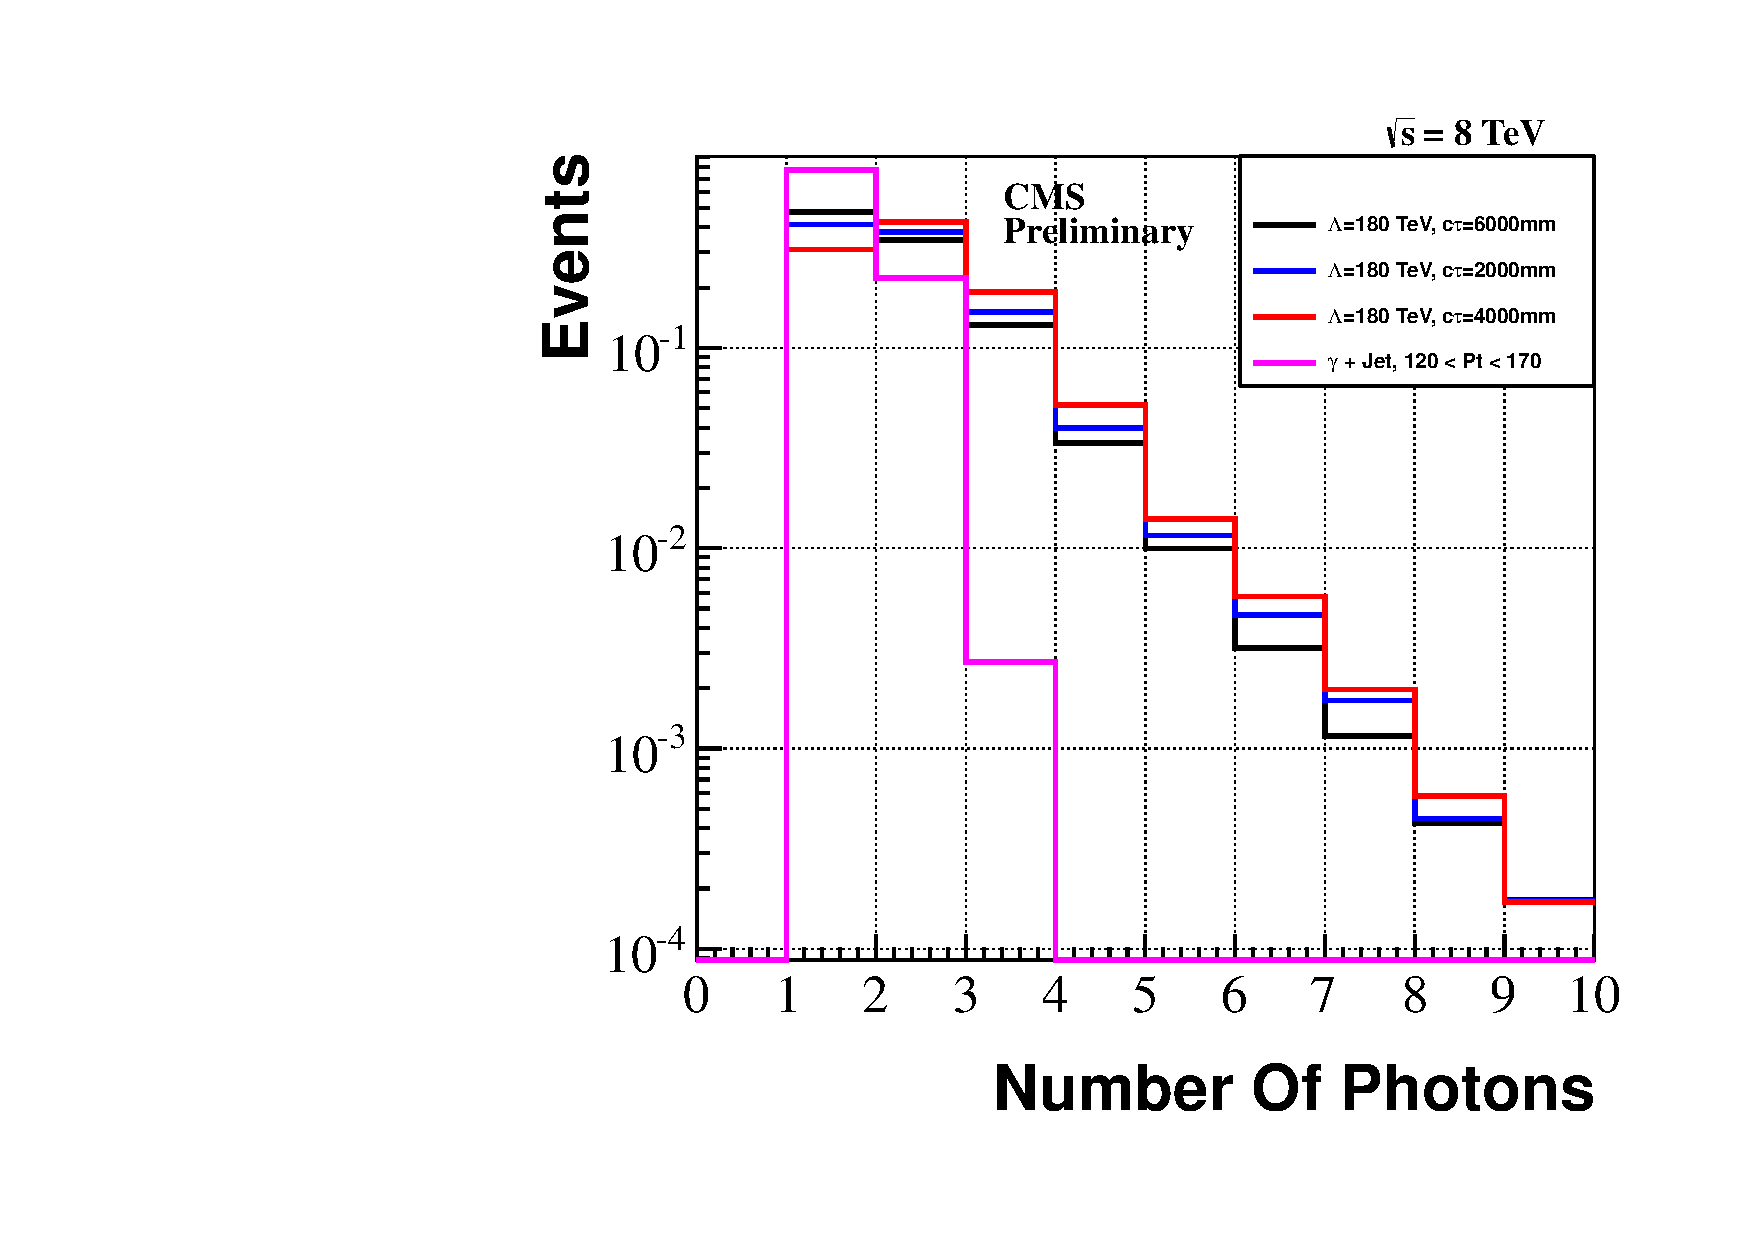
\includegraphics[height=0.5\textwidth,width=0.5\textwidth]{THESISPLOTS/GMSB-SPS8-MODEL-NumberOfPhotons_Lambda-180-TeV.pdf}% \hspace{-1cm}
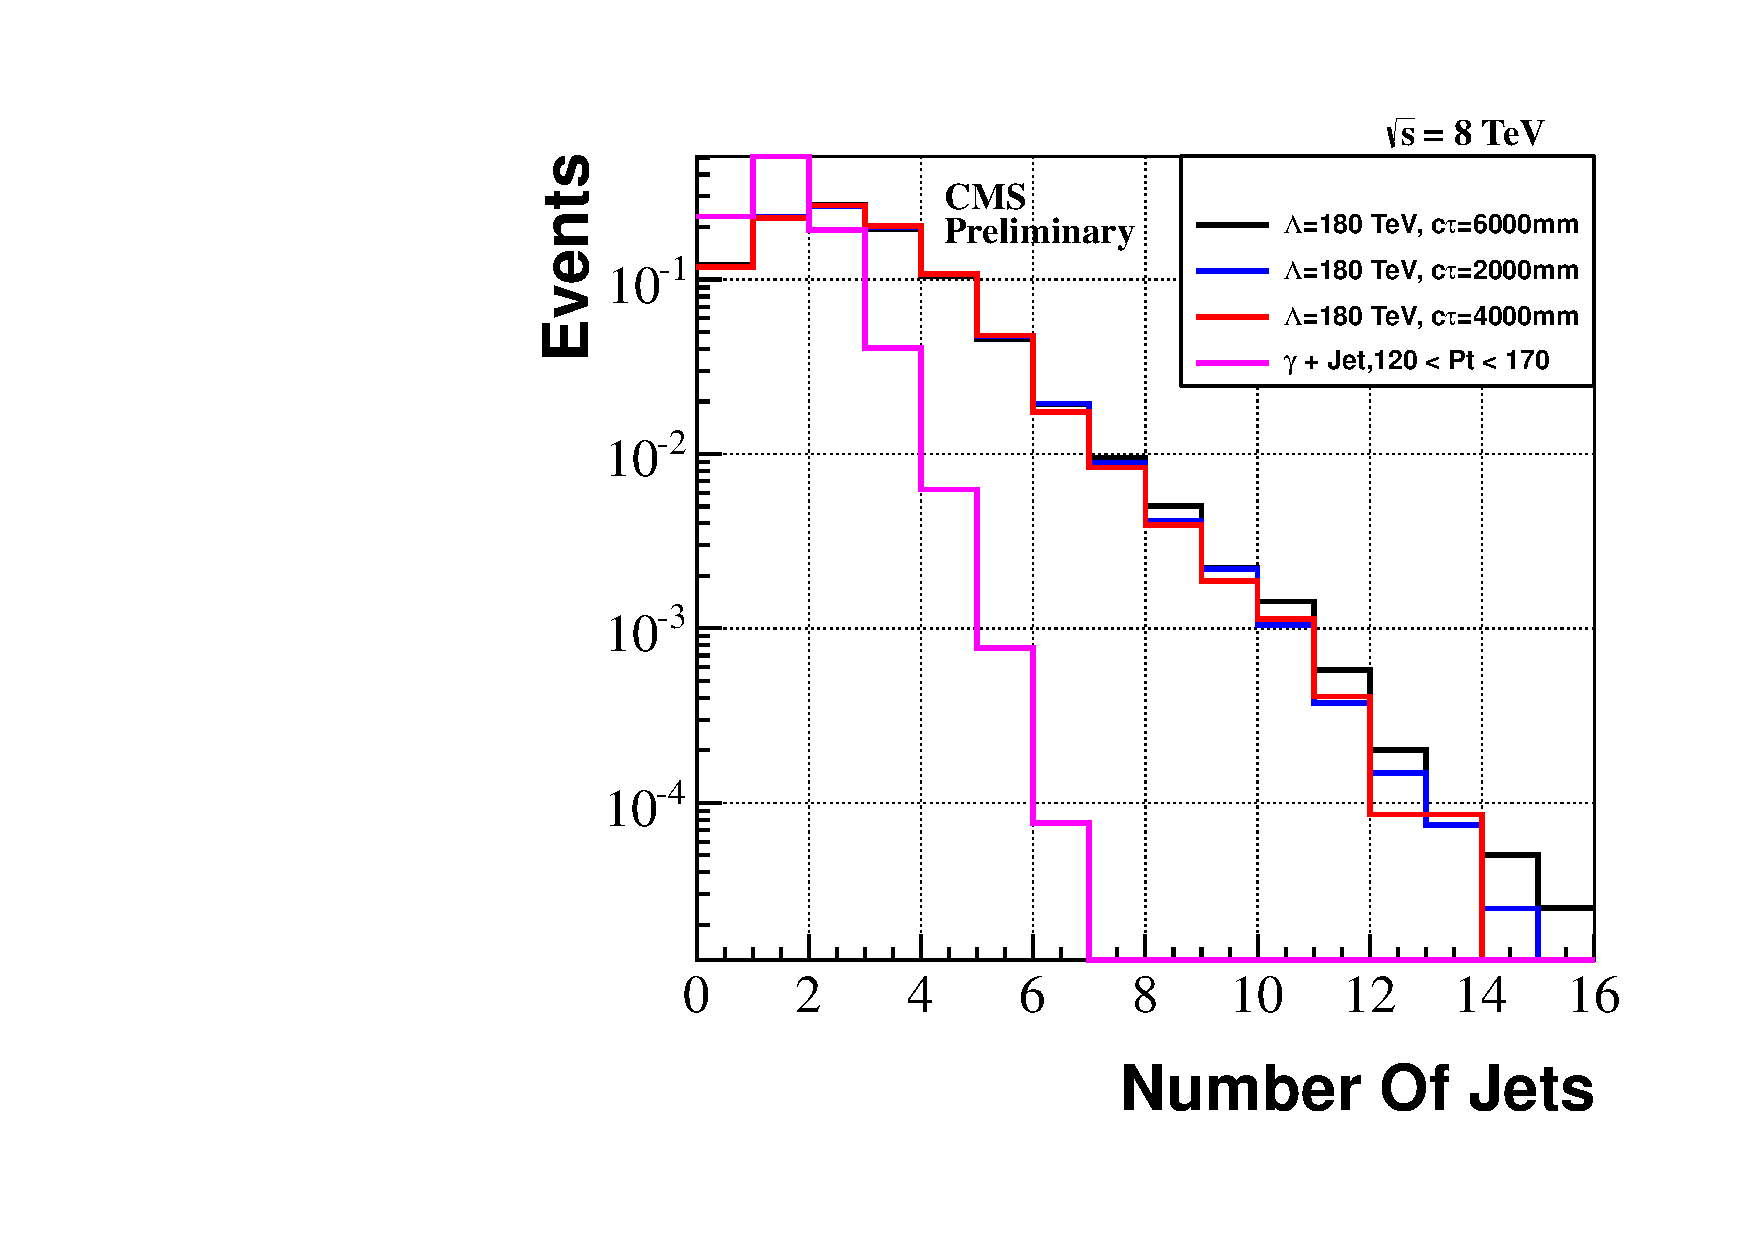
\includegraphics[height=0.5\textwidth,width=0.5\textwidth]{THESISPLOTS/GMSB-SPS8-MODEL-NumberOfJets_Lambda-180-TeV.pdf}} \\
\hspace{0.5cm}
\mbox{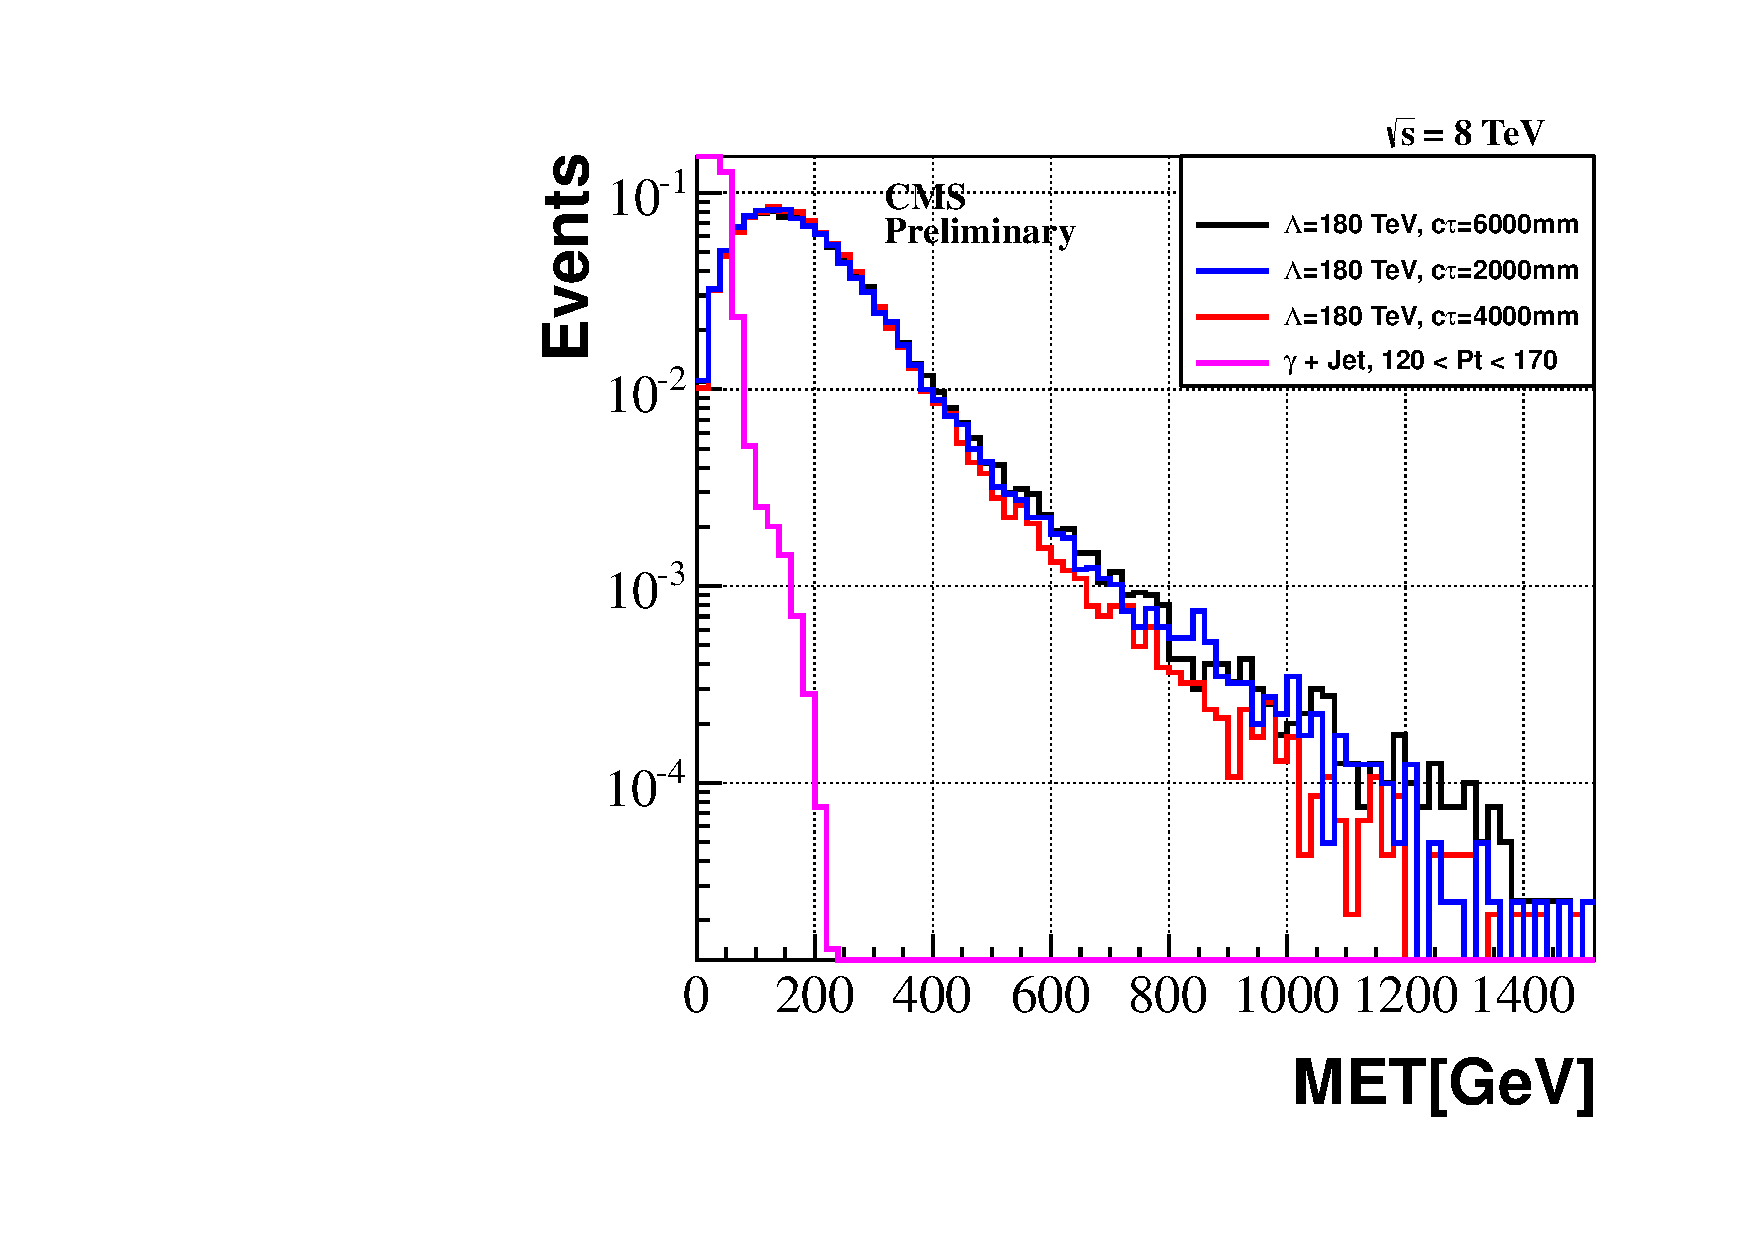
\includegraphics[height=0.5\textwidth,width=0.5\textwidth]{THESISPLOTS/GMSB-SPS8-MODEL-Event-MET_Lambda-180-TeV.pdf}}
\captionof{figure}{Number of photons~(top left),  Number of jets~(top right) and 
\MET~(bottom) for events with \PSneutralinoOne decay to $\gamma$ and $\tilde{G}$ for different $c\tau=2000\mm,4000\mm, 6000\mm$ points of $\Lambda=180$\TeV of the SPS8 model. A $\gamma +$jet with $120 < \hat{\pt} < 170$\GeVc sample shown for comparison with the signal samples.}
\label{fig:NKINE}
\end{center}
\end{minipage}
%%%
\section{ECAL Timing}
In this section, we describe how the photon arrival time is measured, how we adjust the MC time so that it agrees with data. We also described the neutralino lifetime and discuss the possible reasons why the photon is delayed and finally we discuss the satellite bunches and argue that they could be a possible background source to late photons.

\subsection{Photon Time Measurement}
The presence of spikes, noisy crystals and pile-up events, demand a robust method for measuring the photon arrival time at  ECAL and since ECAL time is our main observable for distinguishing background from signal events, such a method must be capable of reducing timing bias which may arise from such anomalous events. As a result, we studied different methods for measuring the photon arrival time at ECAL. 
\newline
The electromagnetic shower of an electromagnetic particle spreads across several crystals~(energy and time measurements from several channels) belonging to the particle's supercluster containing all of the particle's energy. Using the supercluster, the arrival time of an electromagnetic particle can be defined using either the reconstructed time~($ t_{reco}$) of a single crystal, the \textit{seed crystal}~(crystal with the highest energy deposit), or a weighted average time calculated using the reconstructed time and its uncertainty of each crystal of the supercluster. We write, $t_{seed}$, for the seed time and, $t_{Ave}$, for the average time defined as
\begin{equation}{\label{eq:AVETIME}}
t_{Ave} = \frac{\sum_{i=1}^N\frac{t^{i}_{reco}}{\sigma_{i}^{2}}}{\sum_{i=1}^{N}\frac{1}{\sigma_{i}^{2}}},
\end{equation}
where $N$ is the total number of crystals of the supercluster, $t_{reco,i}$  and $\sigma_{i}$ are the time and uncertainty on the reconstructed time of each channel, respectively. 
%Algorithms for extracting and calibrating ECAL crystals using the reconstructed hit~(\textit{rechit}) time have been developed
%and we describe them in detail in the coming sections.
%We use $t_{reco}$ to denote the reconstructed time of each hit or crystal.
%We will denote the calibrated reconstructed time of an electromagnetic object as, $T_{reco}$. 
%Measuring the difference of the ECAL measured time between any two reconstructed objects~(which can be individual crystals or electromagnetic objects) arriving from the same nominal point, which in principle are both expected to have the same time, gives a reliable measurement of the timing resolution of the sub-detector including the crystal-to-crystal synchronization factor.  In ECAL timing, the photon reconstructed time, $t_{reco}$, can be calculated using either of the following methods:
%%\begin{enumerate}
%%\item \textbf{seed time}: The time of the highest energy crystal or hit in the highest energy basic cluster~(about $9$ crystals) of the photon super cluster~(about $25$ crystals). It is denoted 
%%\item \textbf{Average or mean time}: This is the error weighted average time of all the crystals in the photon seed basic cluster.
%%It is denoted as $t_{Ave}$ or $t_{mean}$.
%%\end{enumerate}
%Therefore, the arrival time of a photon or an electromagnetic object, $t_{\gamma}$ or $t_{\Pepm}$, can either be given as $t_{seed}$ or $t_{Ave}$.
Figure \ref{fig:TIME} shows a comparison of a photon time measured as the seed time, $t_{seed}$, and as the average time, $t_{Ave}$. Both distributions have been normalized to total number of events.

\vspace{5mm}
\begin{minipage}{0.90\linewidth} 
\begin{center}
\mbox{
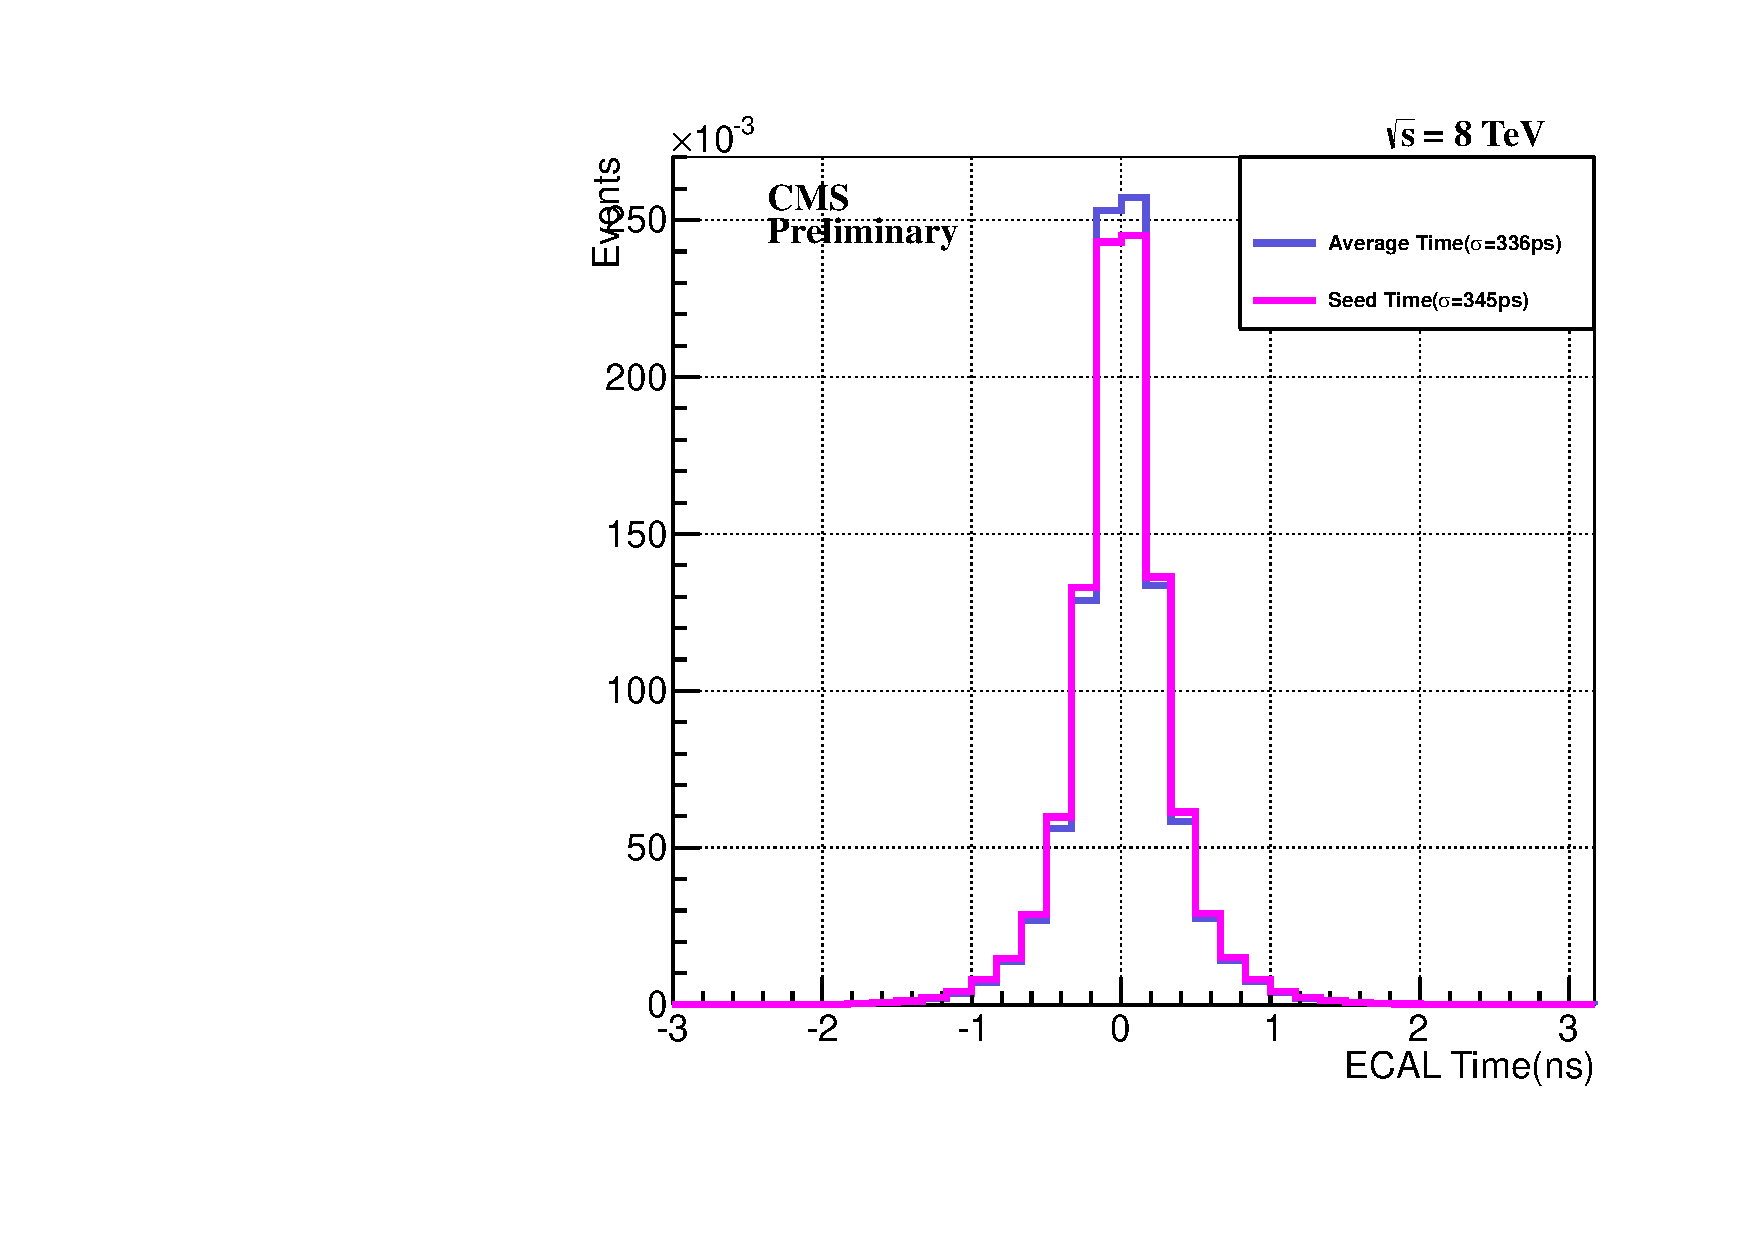
\includegraphics[height=0.50\textwidth, width=0.7\textwidth]{THESISPLOTS/ECAL-SeedVsAveTime-Zee.pdf}
%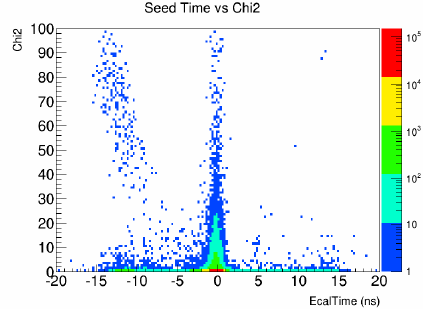
\includegraphics[height=6cm, width=0.5\textwidth]{THESISPLOTS/Seed-Time-Chi2.png}
}
\captionof{figure}{Measuring the photon time using either seed time~(black) or average time~(blue). $\sigma$ of the Gaussian fit from seed time slightly better average time which is computationally intensive.}
\label{fig:TIME}
\end{center}
\end{minipage}

\vspace{5mm}
The width~($\sigma$) of both Gaussian distributions are similar. We observed $\sigma = 345$~ps for the seed time compared to $\sigma = 336$~ps for the average time distributions. 
\newline
In this analysis, we used the seed time for the photon ECAL time. However we also used the $\chi^{2}$ on the photon ECAL time computed using the average time for identifying electromagnetic particles with bad timing. For example, when one or more of the crystals is a supercluster is poorly time calibrated or embedded with a spike, the photon time from the weighted average time measurement can be very biased which is a good reason to  reject such a supercluster.
% A possible solution for this is to select only properly time calibrated crystals of the supercluster for computing the average time or simply used the times from crystals of the \textit{seed basic cluster}. A supercluster is said to consist of many smaller clusters called \textit{basic clusters}, and the average time of the cluster with the highest energy~(seed basic cluster) can also be used as the particle's measured arrival time.
\paragraph*{}
The $\chi^{2}$ on the photon ECAL time calculated as
\begin{equation}\label{eq:CHI2}
\chi^{2} = \sum^{N}_{i=0}\frac{(t^{i}_{reco} - t_{Ave})^{2}}{\sigma_{i}^{2}}
\end{equation}
where, $N$ is the number of crystals in the photon supercluster, $t^{i}_{reco}$ and $\sigma_{i}$ are the time and uncertainty on the reconstructed time for each crystal and $t_{Ave}$ is the mean time defined in Equation \ref{eq:AVETIME}, is a reliable quantity to legitimized the photon time and to distinguish fake photons~(jets misidentified as photons) and spikes from true photons. Figure  \ref{fig:spikeVsPhoton} shows the profile of the pulse shape~(left) of an identified spike with that of a true photon. A distribution of the normalized $\chi^{2}$ against the ECAL time is also shown in the right plot of the same figure. Photons with a signal pulse shape profile as that of spikes are associated with large values of $\chi^{2}$ and usually have negative ECAl time.
 
 \vspace{5mm}
%\paragraph*{}\mbox{}\\ 
\begin{minipage}{0.90\linewidth} 
\begin{center}
\mbox{
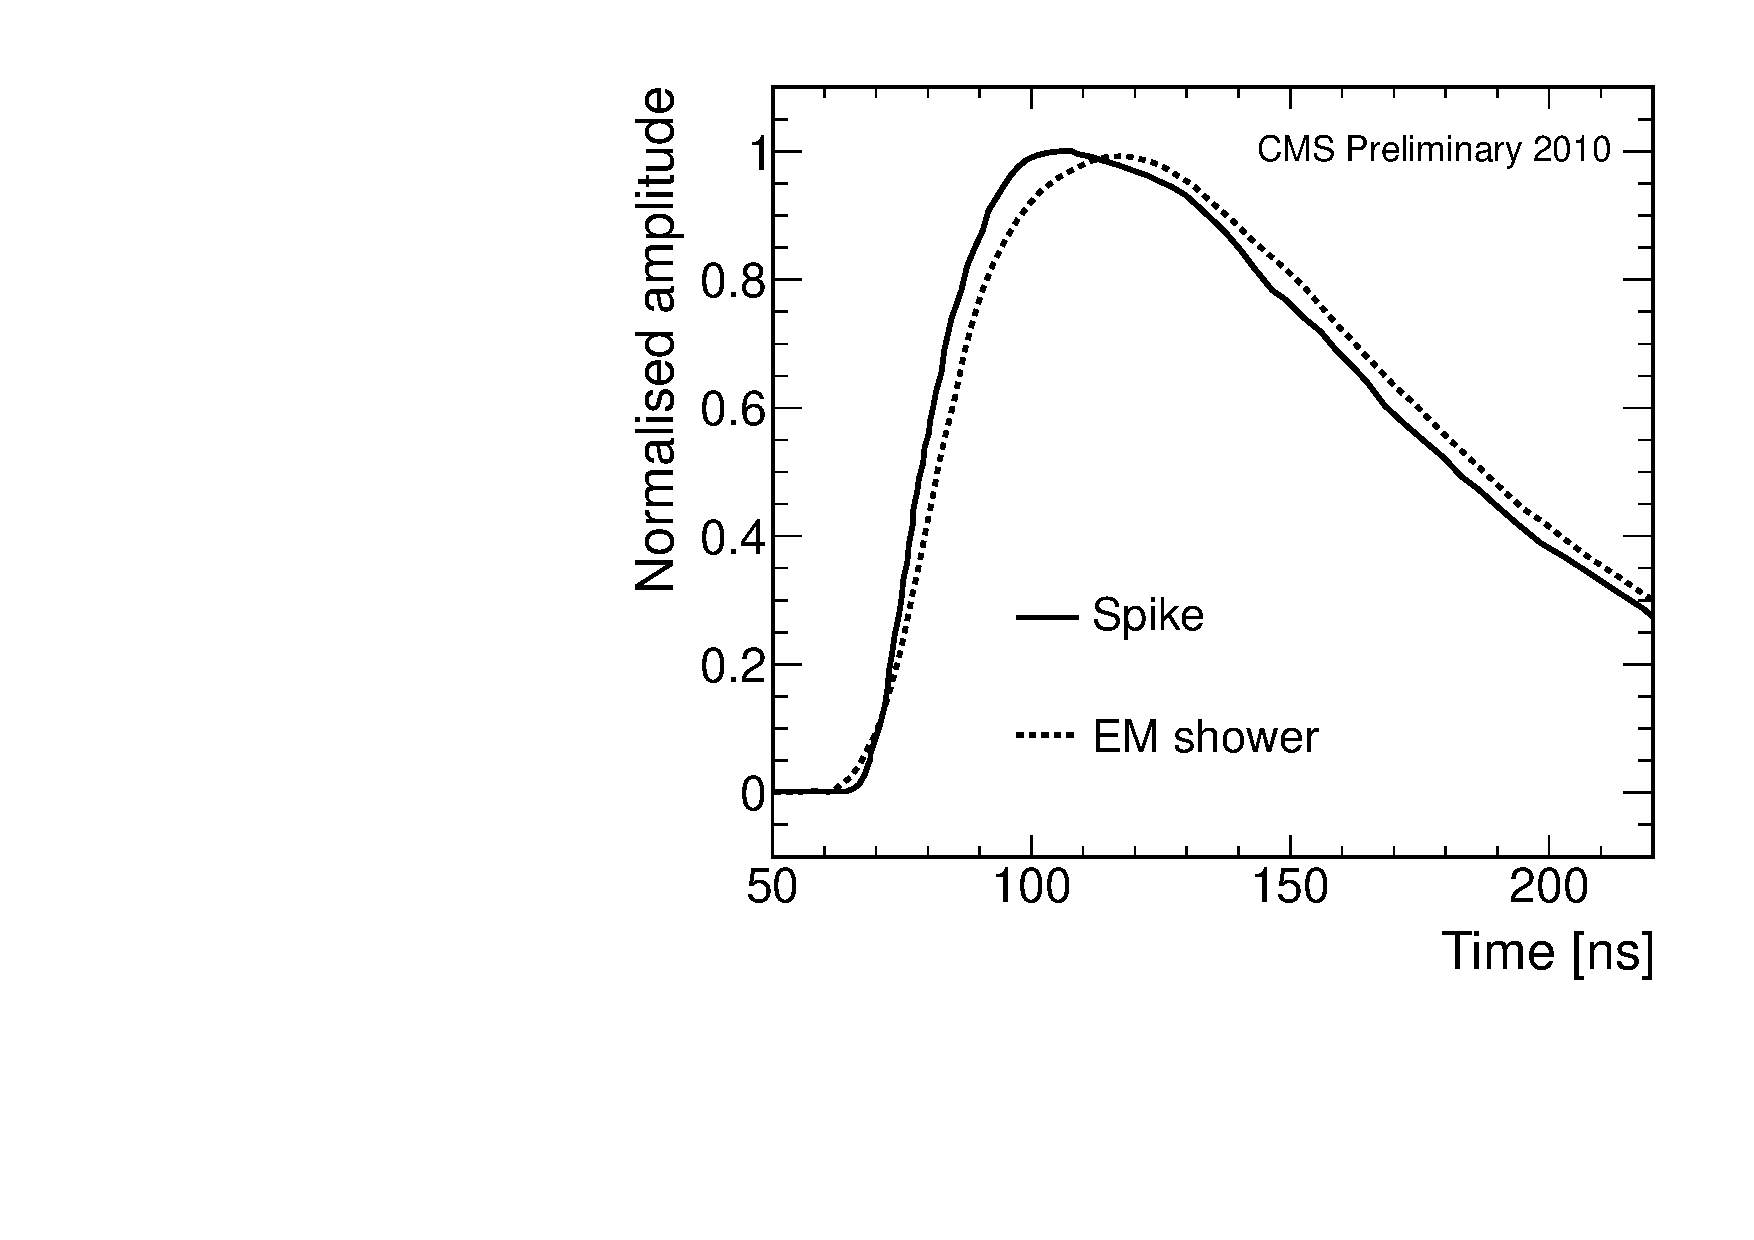
\includegraphics[height=.450\textwidth, width=0.45\textwidth]{THESISPLOTS/spike_pulse_shape.pdf}
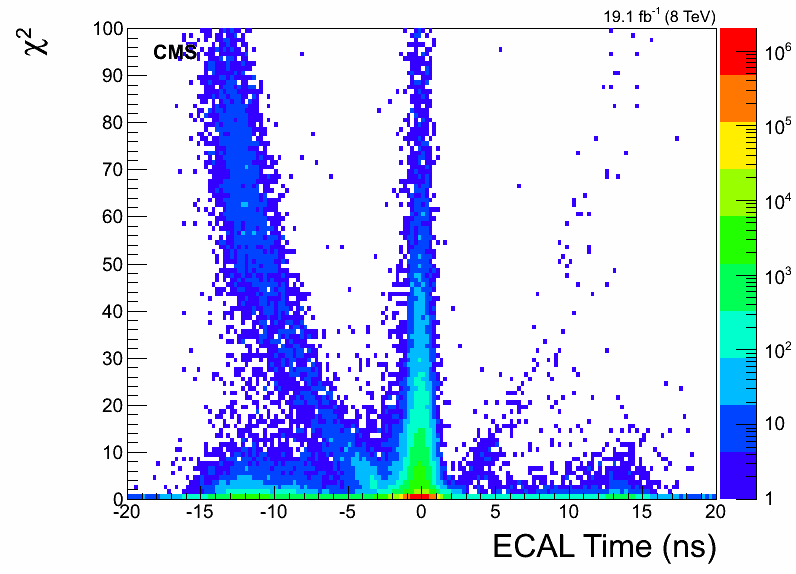
\includegraphics[height=.450\textwidth, width=0.5\textwidth]{THESISPLOTS/seedTime_Chi2.png} }
\captionof{figure}{Pulse shape profile(left) showing a spike~(solid line) and a true EM shower~(dashed line) from data. The $\chi^{2}$ against ECAL time  distribution(right) shows spikes misidentified as photons with very large $\chi^{2}$ and negative ECAL time. The region of $\chi^{2} > 4$ is mostly dominated by spikes events.}
\label{fig:spikeVsPhoton}
\end{center}
\end{minipage}

 \vspace{5mm}
From the $\chi^{2}$ $Vs$ ECAL time plot~(right plot of Figure \ref{fig:spikeVsPhoton}), we observe that  most of the photons have ECAL time around zero but also many of the photons with large ECAL time  have large normalized $\chi^{2}$ values which is expected where the time measurements by non-seeded crystals is inconsistent with the time measurement of the seed crystal. We also observed that, a cut in $\chi^{2} < 4$, can reduce with 99.2\% efficiency, photon contributions from spikes and misidentified jets where a neutron embedded in the jet hitting directly the photo-detectors produces a spike.
%%%
%%%%
\subsubsection{Monte Carlo Time}
It is challenging to properly simulate ECAL time for MC events so that it captures the conditions of the ECAL detector during data recording. As a result, the time from MC events does not entirely represent the status of ECAL time in data, in terms of mean time and time resolution.
We extract the adjustments for MC event time needed to match the mean time and timing resolution of data using a MC $\gamma +$jet samples of selected 1 or 2-jets events. Only events with isolated in-time, $t_{\gamma} < 2$~ns, with $\pt > 80$\GeV are selected. 
We perform the adjustment by shifting the mean time and smearing the timing resolution by an additional Gaussian convolution on the photon time of MC events so as to match the mean time and time resolution of data. The photon ECAL time from data and MC $\gamma +$jet samples both shown in Figure \ref{fig:DATAMCTime}; where we compare before~(left plot) and after~(right plot) the adjustment on MC ECAL time was made, agree quite well. 
%We performed the same smearing for all MC samples used in our analysis.
%\newline
% It is worth noting that the difference of 125~ps between $t^{MC}_{reco}$ and $t^{DATA}_{reco}$ compared to 500~ps ECAL timing resolution is not enough to enormously impact our event selection. %however, simulating photons ECAL time in the tails of the time distribution still remains.

\vspace{5mm}
%\paragraph*{}\mbox{}\\
\begin{minipage}{0.90\linewidth} 
\begin{center}
\centering
\mbox{
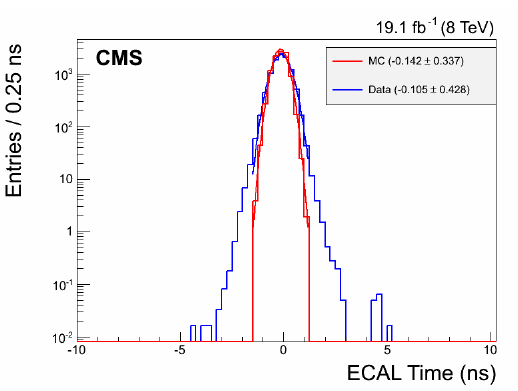
\includegraphics[height=0.5\textwidth, width=0.5\textwidth]{THESISPLOTS/MC_Vs_DataTimeB4Calib.png}
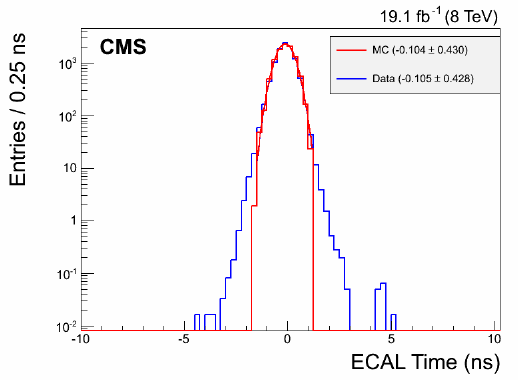
\includegraphics[height=0.5\textwidth, width=0.5\textwidth]{THESISPLOTS/MC_Vs_DataTimeAferCalib.png}
}
\captionof{figure}{ECAL time distributions of in-time photons from MC $\gamma +$ jets~(blue)  and data~(red) samples before~(left) and after~(right) we adjusted the photon time from MC.}
\label{fig:DATAMCTime}
\end{center}
\end{minipage}
%%%
%\clearpage
\subsection{Neutralino Lifetime}
The distance traveled, in the CMS detector, by the \PSneutralinoOne before it decays,  mentioned previously section \ref{NeutralinoDecay}, is given as
\begin{equation}{\label{eq:decaylength}}
\mathrm{L} = \left(c\tau_{\PSneutralinoOne}\right) \cdot \left( \gamma \beta\right) = \left(c\tau_{\PSneutralinoOne}\right) \cdot \left( \frac{p}{m_{\PSneutralinoOne}}\right).
\end{equation} 
This distance depends on the momentum~($p$) and mean lifetime~($c\tau_{\PSneutralinoOne}$) of the \PSneutralinoOne. Large values of $c\tau_{\PSneutralinoOne}$ means, this distance is large and if larger than the ECAL radius, can be interpreted as the \PSneutralinoOne traveled outside the ECAL volume before it decayed, making detecting the delayed photon no longer possible. On the other hand, small values of $c\tau_{\PSneutralinoOne} < 10\cm $ means the \PSneutralinoOne decayed early and the photon is not late enough such that its detection using ECAL time measurements alone is not reliable. High-$p$ values means the \PSneutralinoOne is boosted and could travel out of the ECAL before it decay,  making the photon again undetectable. On the other hand, low-$p$ values means the \PSneutralinoOne is less boosted and traveling slow enough for its decay to happen inside the ECAL volume and the photon delayed arriving at ECAL. In Figure \ref{fig:NKINE}, we show a distribution of the momentum of the \PSneutralinoOne in the transverse~($x-y$) plane~(transverse momentum~( $\pt^{\PSneutralinoOne}$)), the \PSneutralinoOne transverse distance traveled before it decay, the transverse momentum of the photon~($\pt^{\Pphoton}$) and photon's estimated time~($T_{\Pphoton}$) using only generator level information. These distributions are for different $\Lambda$ and $c\tau_{\PSneutralinoOne}$ points of the SPS8 model. We observed that, the $\pt^{\PSneutralinoOne}$ increases with increase values of $\Lambda$, from $\Lambda = 100\TeV$ to 220\TeV, which agrees with our expectation. As $\Lambda$ increases along with the masses of the gluino/squark and \PSneutralinoOne,  the $\pt^{\PSneutralinoOne}$ also increases since a massive gluino/squark decay into the \PSneutralinoOne. In the same way, increasing the mass of \PSneutralinoOne ~($m_{\PSneutralinoOne}$) through increasing $\Lambda$, leads to increase in the photon \pt. For a given value of $\Lambda=180\TeV$, which means $\pt^{\PSneutralinoOne}$ is fixed, the transverse distance traveled by the \PSneutralinoOne before decay~(shown in the top right plot of Figure \ref{fig:NKINE}) and photon time~(shown in the bottom right plot of the same figure) increased with increasing value of \PSneutralinoOne mean lifetime, $c\tau = 50\cm$ to $600$\cm in the same way, qualitatively. These observations support our expectation that the photon is delayed primarily because of the long lifetime of the \PSneutralinoOne. However, one can argue that this is not entirely true and we will exploit this further in a detailed study of the source of delayed photons in the next section.

\vspace{5mm}
\begin{minipage}{0.95\linewidth} 
\begin{center}
\mbox{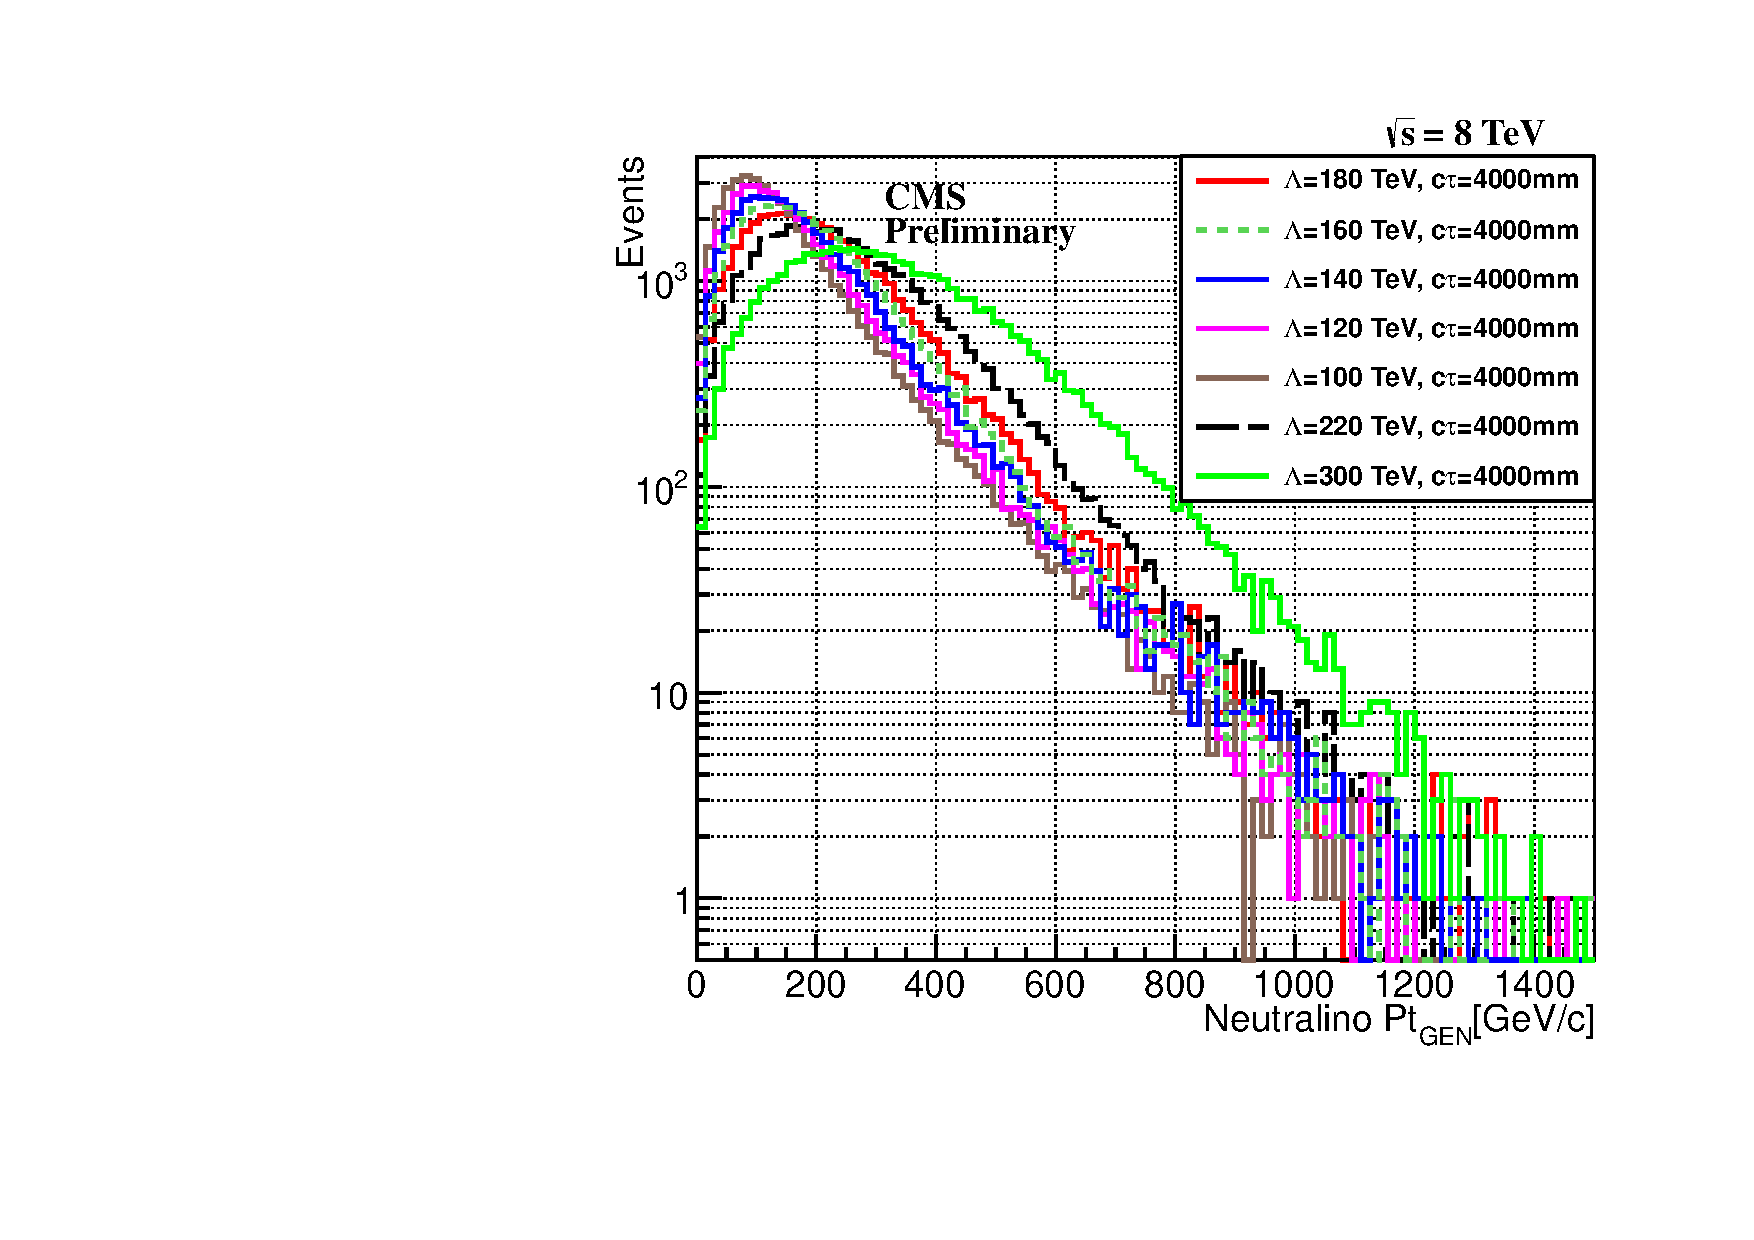
\includegraphics[height=0.45\textwidth,width=0.5\textwidth]{THESISPLOTS/GMSB-SPS8-MODEL-Neutralinio-Pt_ctau-4000-mm.pdf} %\hspace{-1cm}
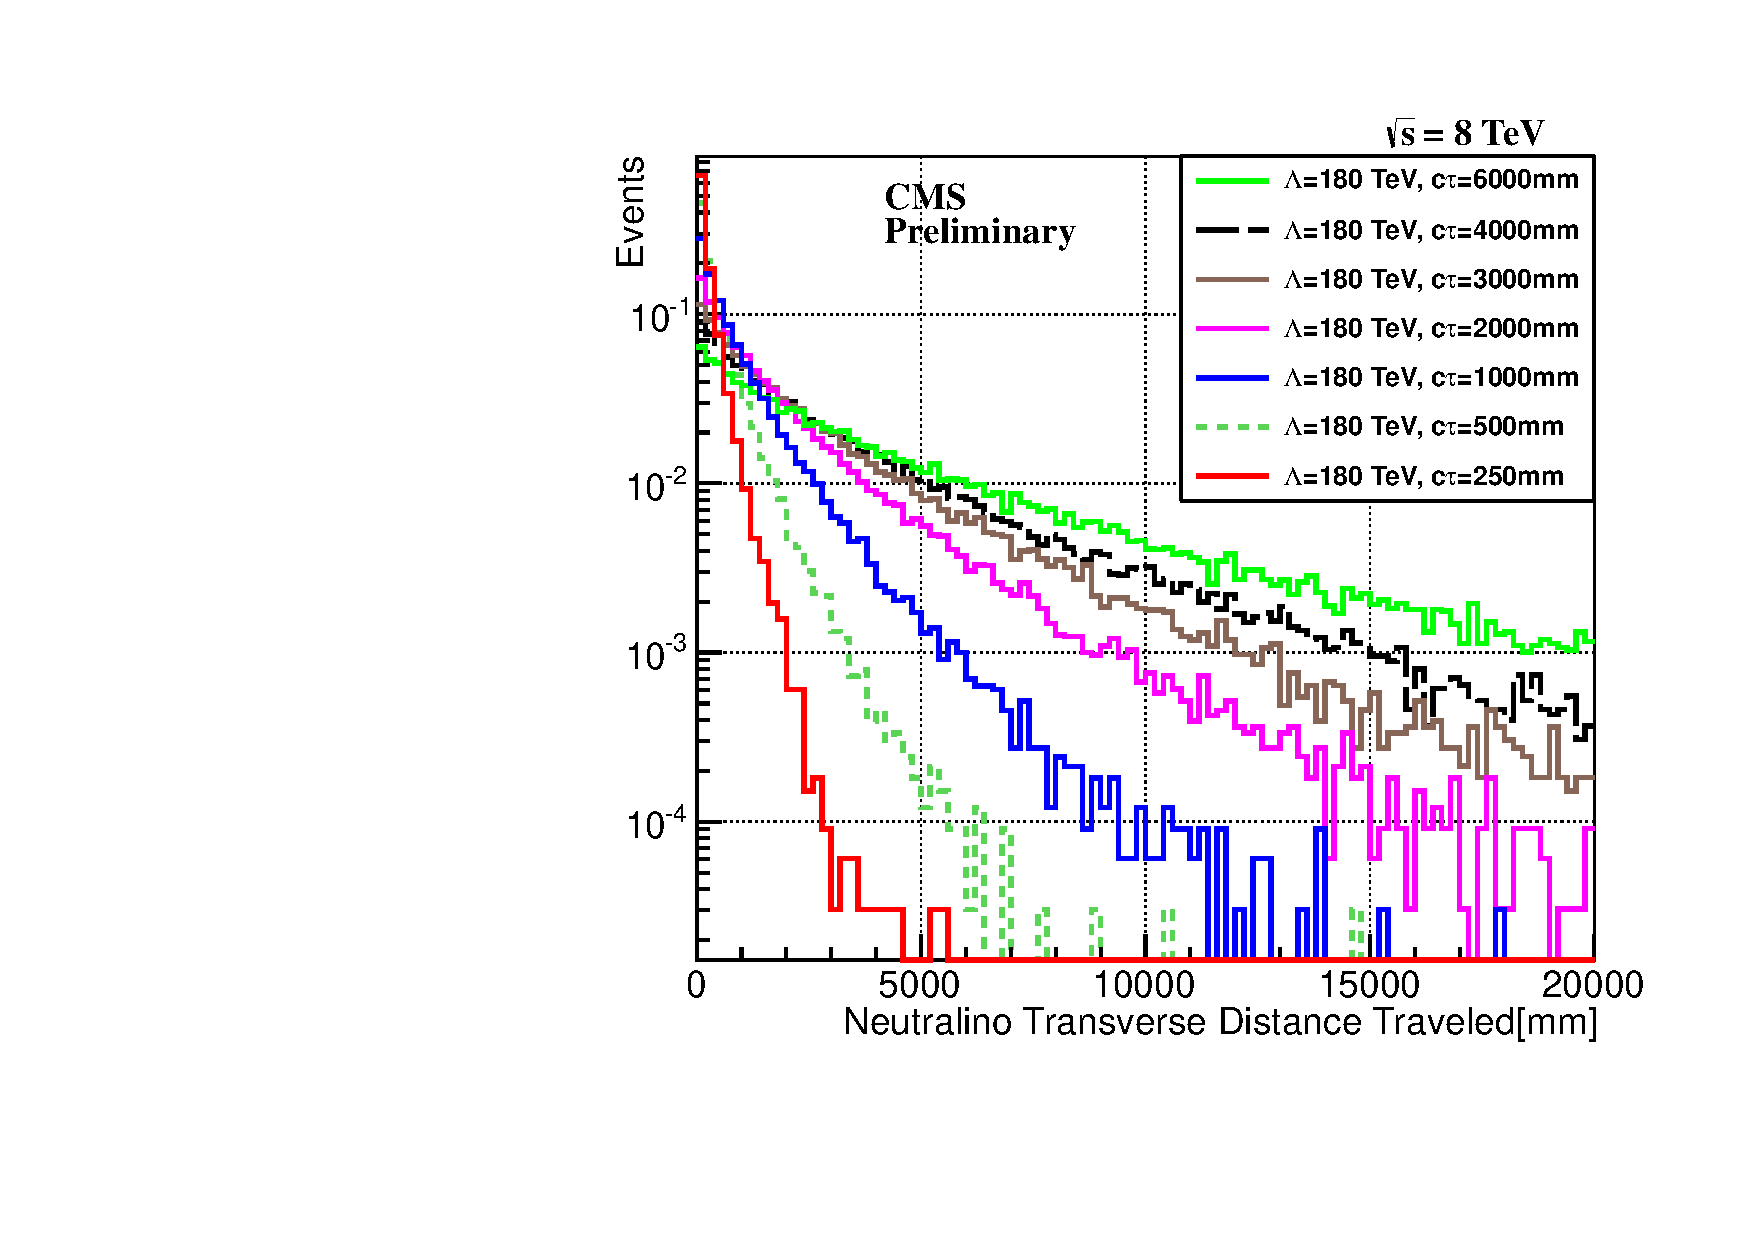
\includegraphics[height=0.45\textwidth,width=0.5\textwidth]{THESISPLOTS/GMSB-SPS8-MODEL-Neutralino-Proper-DecayLength_Lambda-180-TeV.pdf}} \\
\hspace{0.5cm}
\mbox{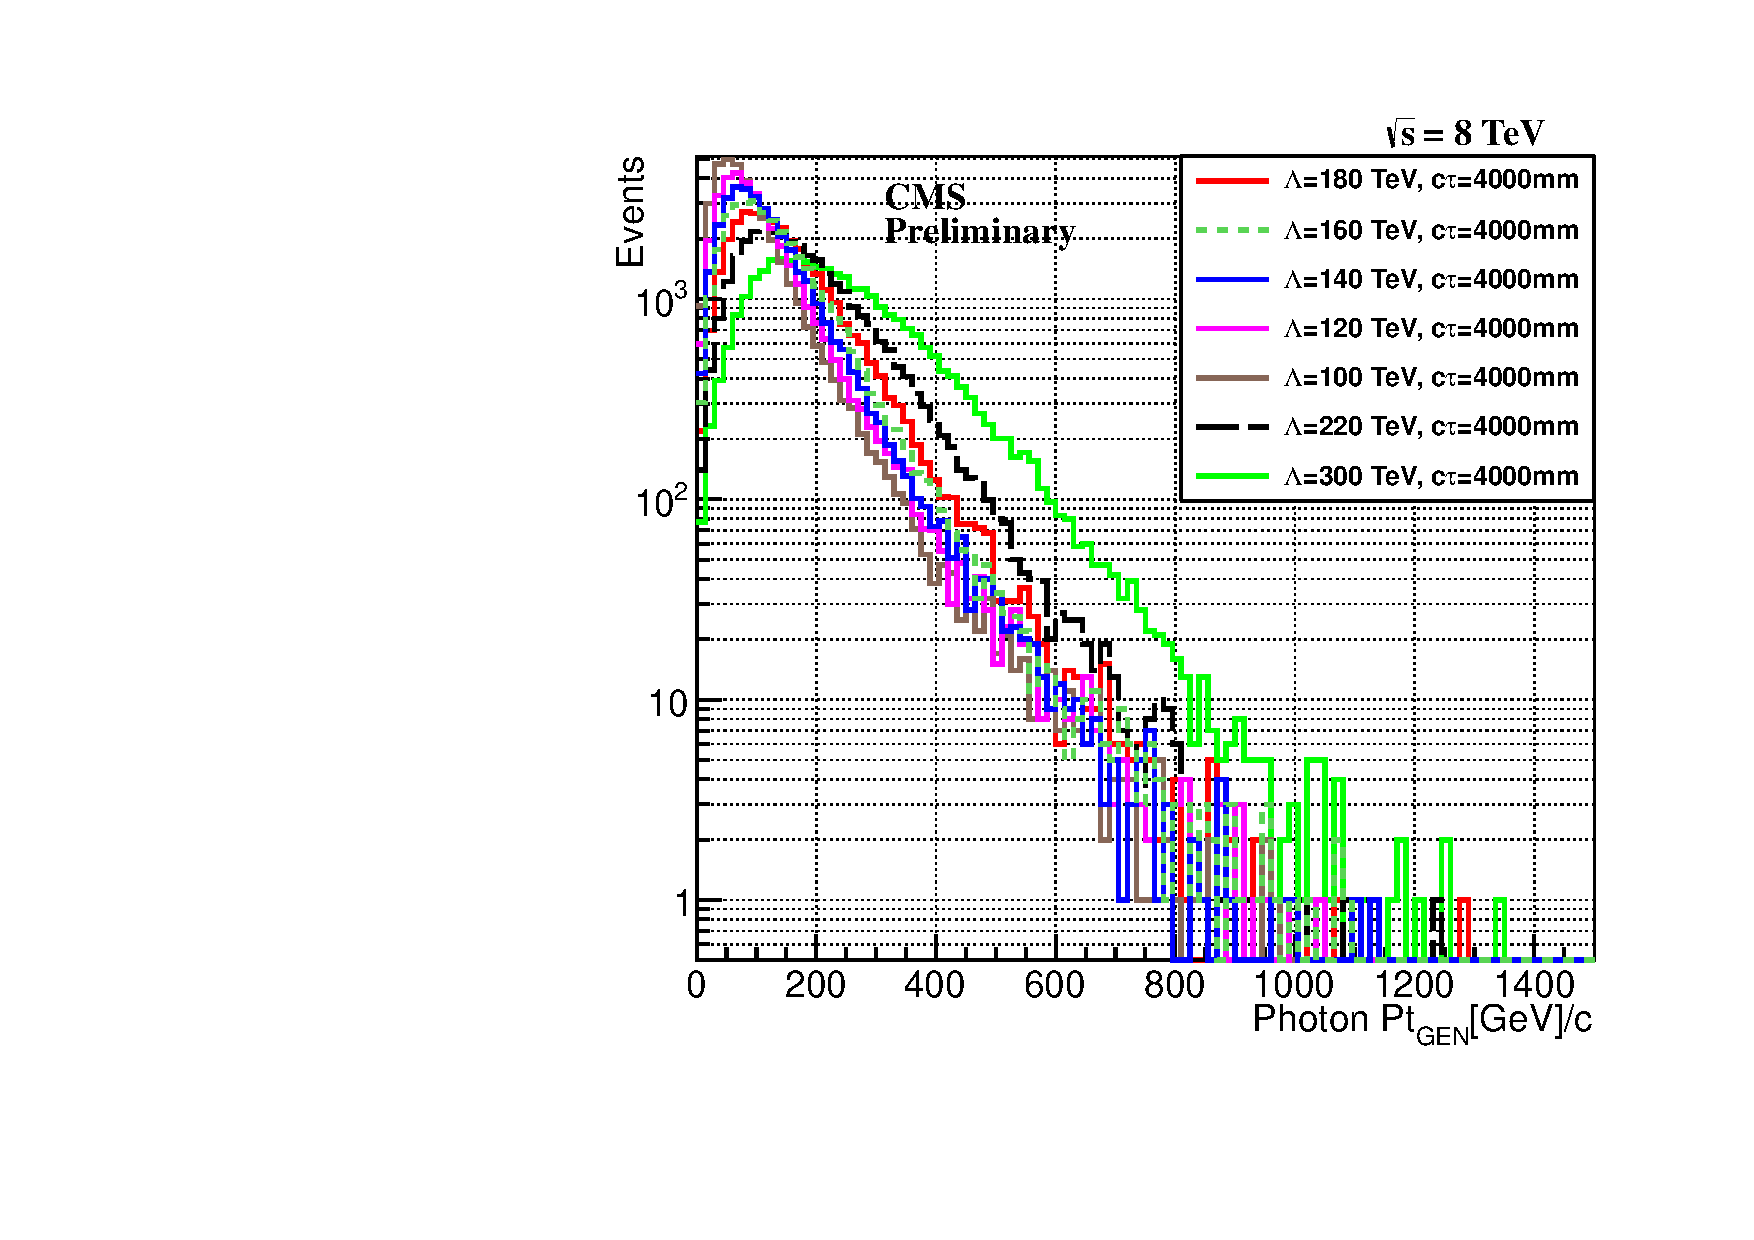
\includegraphics[height=0.45\textwidth,width=0.5\textwidth]{THESISPLOTS/GMSB-SPS8-MODEL-Photon-Pt_ctau-4000-mm.pdf} %\hspace{-1cm}
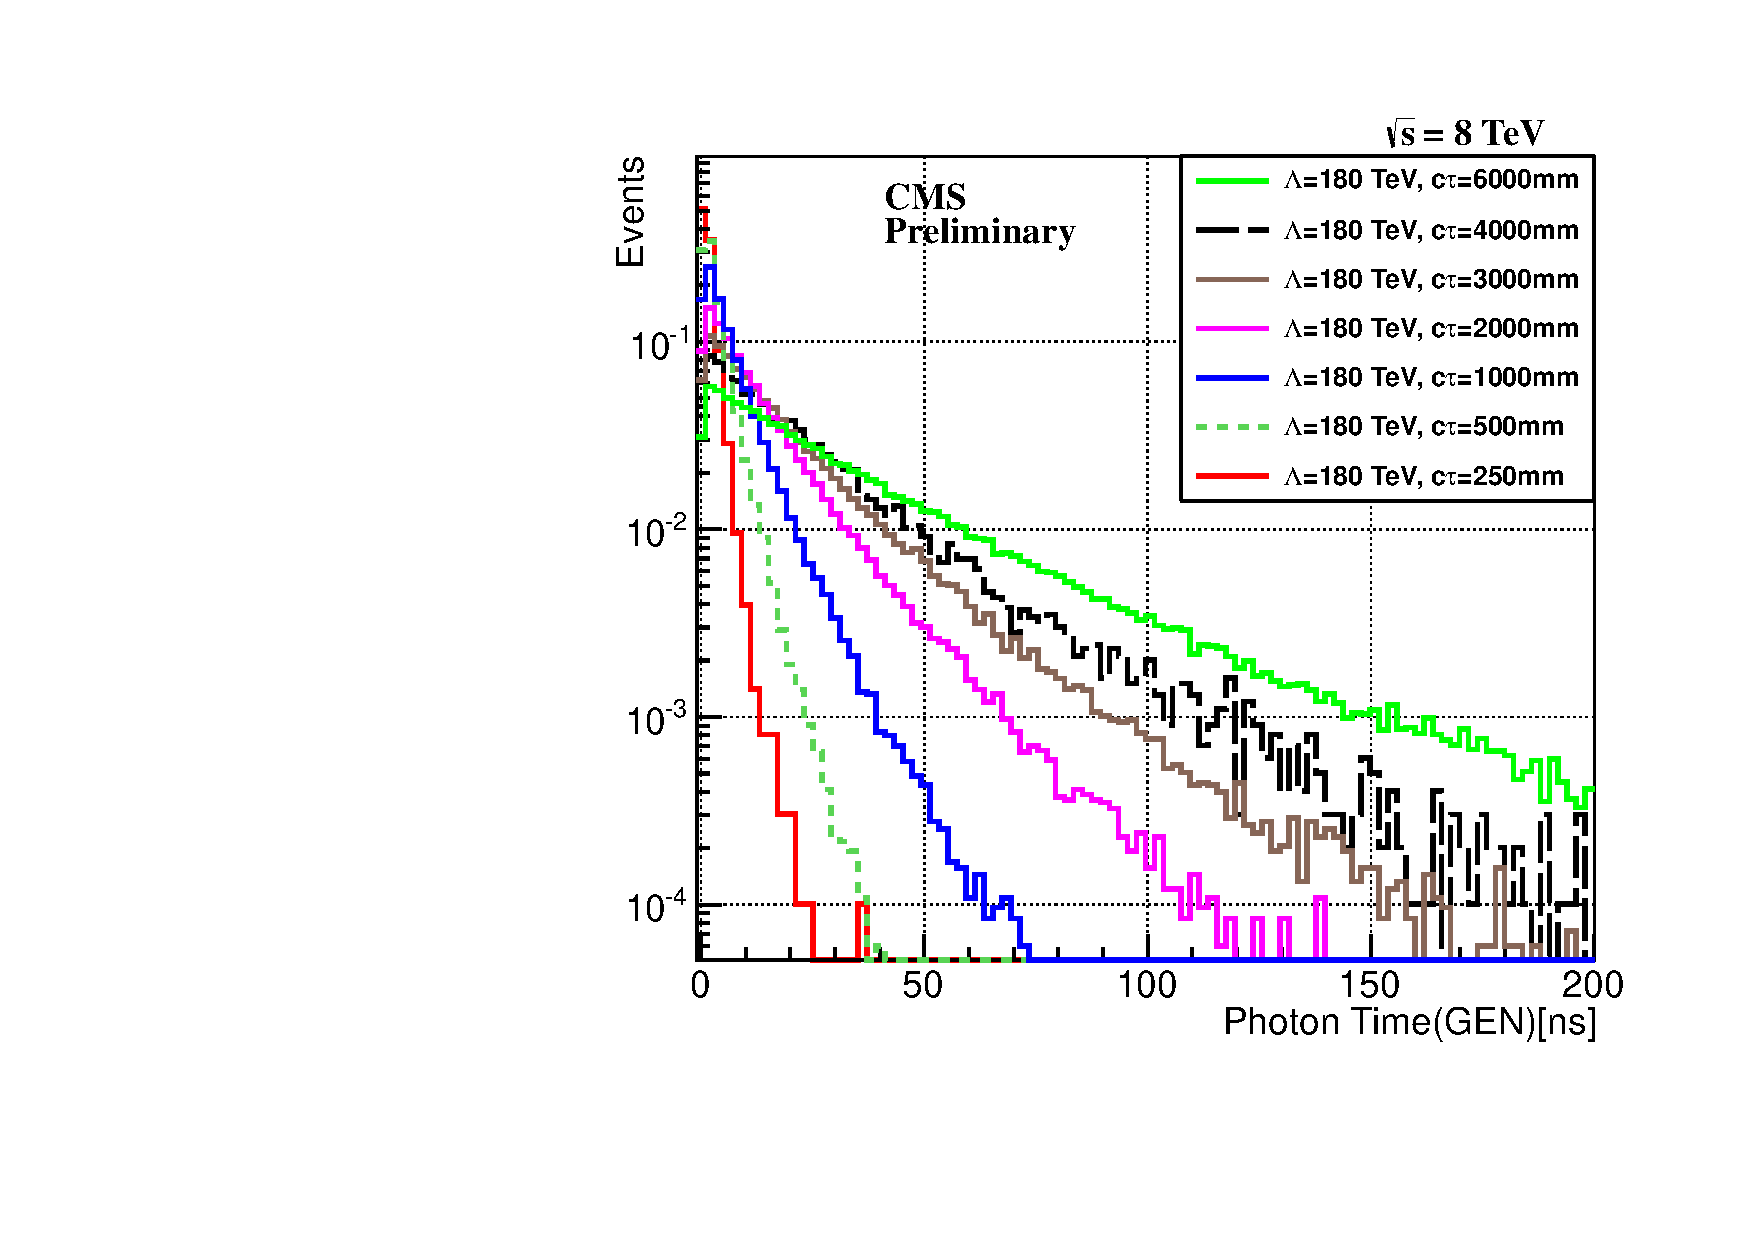
\includegraphics[height=0.45\textwidth,width=0.5\textwidth]{THESISPLOTS/GMSB-SPS8-MODEL-Photon-GEN-Time_Lambda-180-TeV.pdf}}
\captionof{figure}{Neutralino transverse momentum~($\pt^{\PSneutralinoOne}$) distribution~(top left) and transverse distance traveled~(top right). Transverse momentum~(bottom left) and time~(bottom right) of photon from neutralino decay for different $\Lambda$ and $c\tau$ points in GMSB SPS8 model.}
\label{fig:NKINE}
\end{center}
\end{minipage}
 
%%\subsubsection{Source of Delayed Photons}
\vspace{5mm}
The photon from the decay of \PSneutralinoOne can arrive late at ECAL for either one of the following reasons: first, because the \PSneutralinoOne is traveling slow \ie with boost, $\beta = \frac{p_{\PSneutralinoOne}}{m_{\PSneutralinoOne}} << 1$, and second, because the \PSneutralinoOne was produced with significant boost such that the photon traveled to ECAL through a non-direct flight path from the nominal $pp$ interaction point. We distinguish between these two sources of delayed photons by estimating the photon arrival time at ECAL in each scenario using the  distance traveled by \PSneutralinoOne before decay and the distance traveled by the photon from the decay point to the point of detection at ECAL. Figure \ref{fig:DELAY}~(left) is a schematic representation showing how we estimate the photon arrival time at ECAL in each of the possible travel flight path representing the different source of delayed photons. The estimated photon arrival ECAL time in each scenario is given as follows:
\begin{itemize}
  \item For slow moving neutralinos: $\Delta t_1$ = (L1/c$\beta$) - (L1/c)
  \item For non-direct traveled flight path: $\Delta t_2$ = (L1 + L2 - L3)/c
  \item ECAL measured time = $\Delta t_{1} + \Delta t_{2}$
\end{itemize}
%\newline
\begin{minipage}{0.90\linewidth} 
\begin{center}
\mbox{
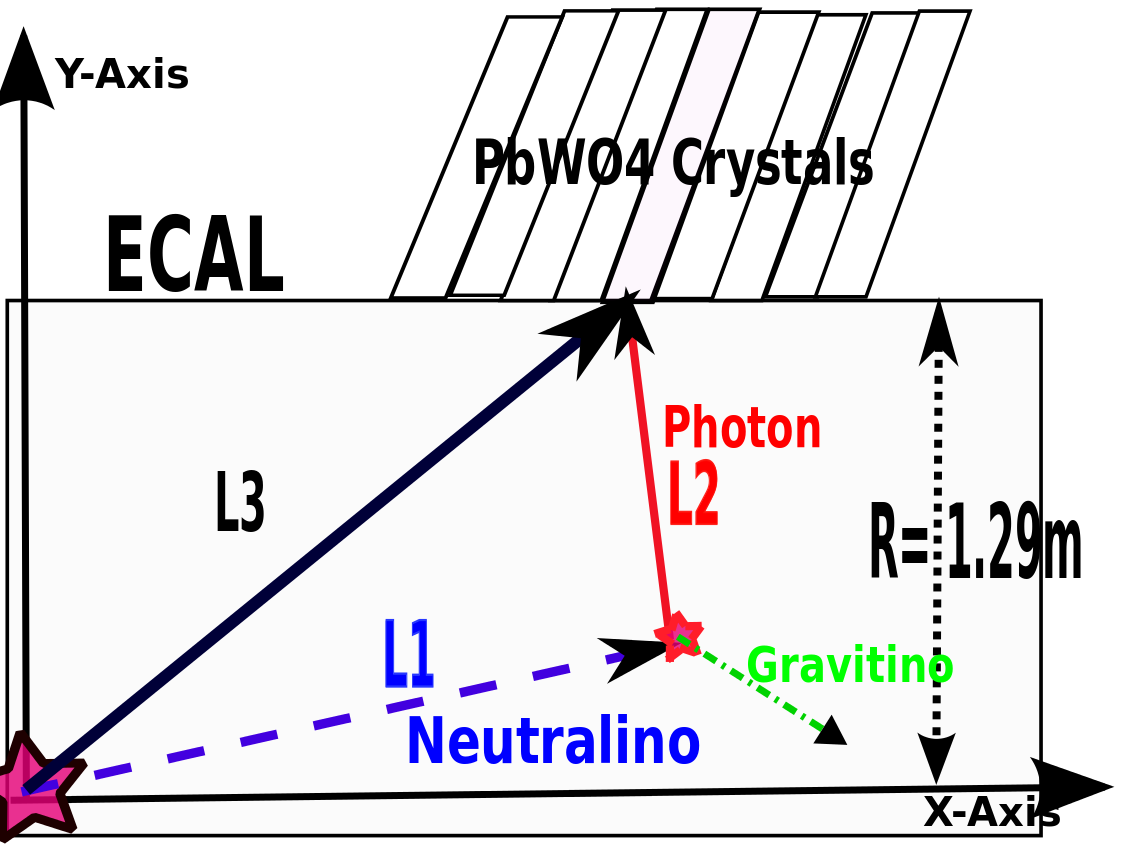
\includegraphics[height=0.55\textwidth, width=0.5\textwidth]{THESISPLOTS/DelayedPhoton-ECAL.png}
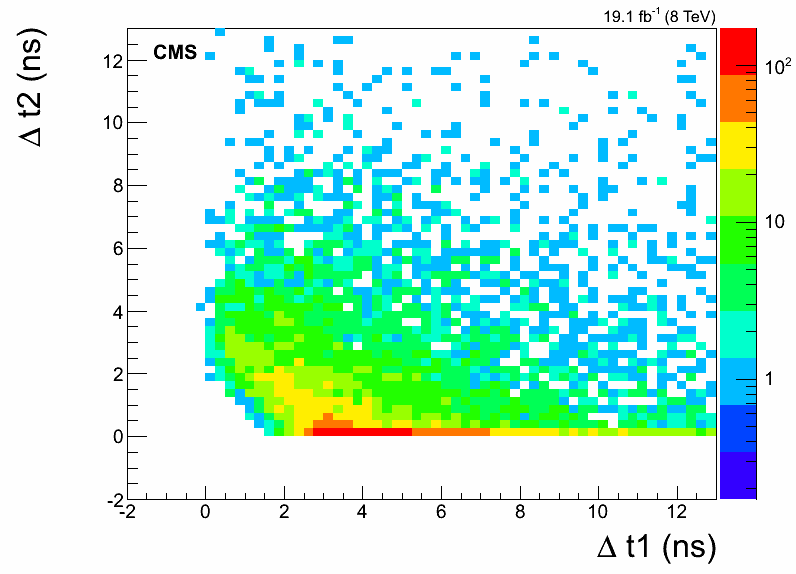
\includegraphics[height=0.55\textwidth, width=0.5\textwidth]{THESISPLOTS/dt1_dt2_late.png}
}
\captionof{figure}{Schematic diagram showing $\tilde{\chi}^{0}_{1} \rightarrow \gamma + \tilde{G}$ decay topology within the ECAL volume of the CMS detector~(\textit{Left}). The estimated photon arrival time at ECAL  from the decay of \PSneutralinoOne in the SPS8 model with $m_{\PSneutralinoOne}=256$\GeVcc and $c\tau = 600$\cm~(\textit{Right}).}
\label{fig:DELAY}
\end{center}
\end{minipage}

\vspace{5mm}
The \PSneutralinoOne is traveling with velocity, $v = c\beta$, where $c$ is the speed of light in vacuum. The distribution of the estimated photon ECAL arrival times $\Delta t_{1}$ and $\Delta t_{2}$, is plotted shown in Figure \ref{fig:DELAY}(right), where the color intensity represents the photon population. We observed that most of the late arrival time photons are from the decay of slow moving \PSneutralinoOne compared to those from non-direct flight path to ECAL. This proves that a good number of \PSneutralinoOne produced with low momentum such that the ratio $\frac{p_{\PSneutralinoOne}}{m_{\PSneutralinoOne}} << 1$ produced most of our detectable delayed photons, using ECAL time measurements. While \PSneutralinoOne with very long lifetimes~($c\tau$) produced with high momentum will very likely escape the ECAL without detection unless their decay happens within the ECAL volume such that the delayed photon arrives at the ECAL in a non-direct flight path.
%%%%%
\subsection{Satellite Bunches}
We observed~(see Figure \ref{fig:TIMEECAL}) a 2.5~ns discrete pattern in the photon ECAL time of events, produced in $pp$ collisions, with photon $\pt > 50$\GeVc and belonging to the barrel and endcaps.

\begin{minipage}{0.90\linewidth} 
\begin{center}
\centering
\mbox{
%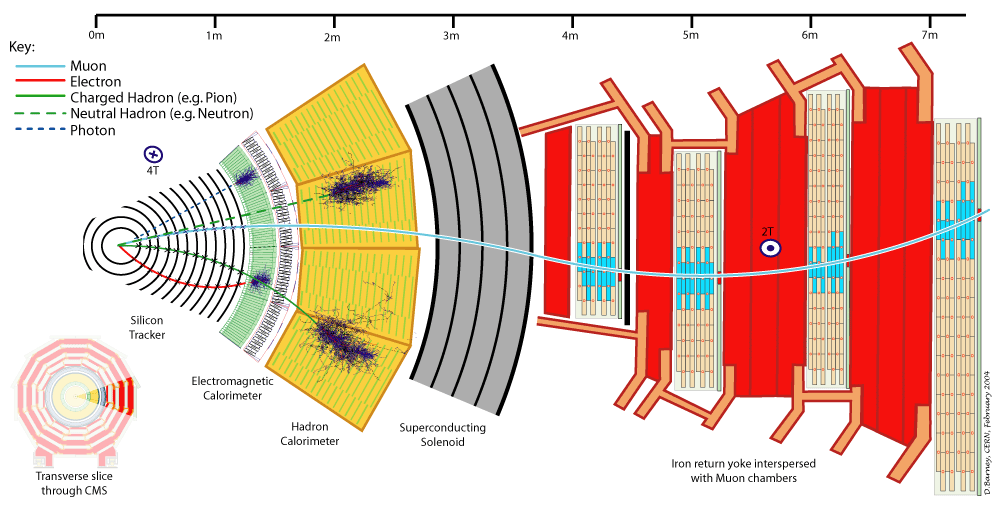
\includegraphics[scale=0.2]{THESISPLOTS/CMS_Slice.png}
%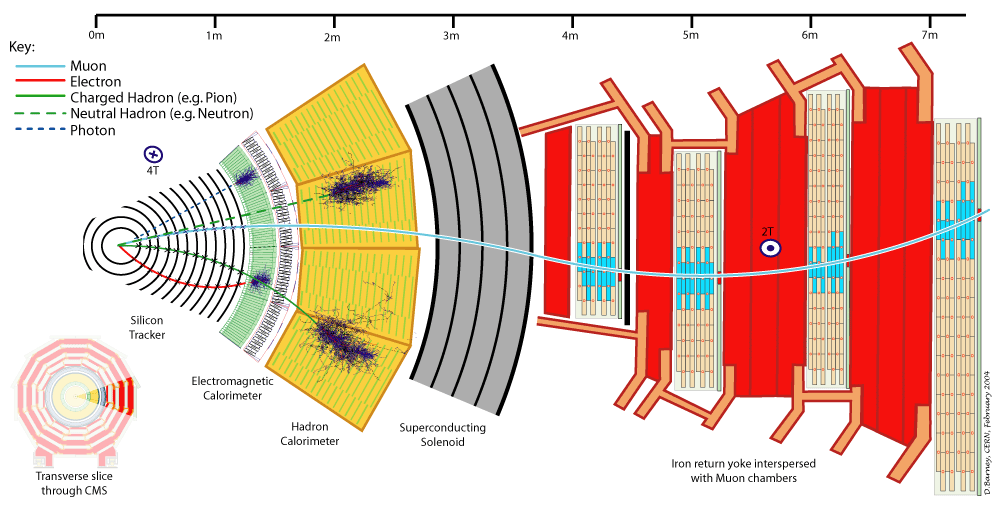
\includegraphics[scale=0.2]{THESISPLOTS/CMS_Slice.png}
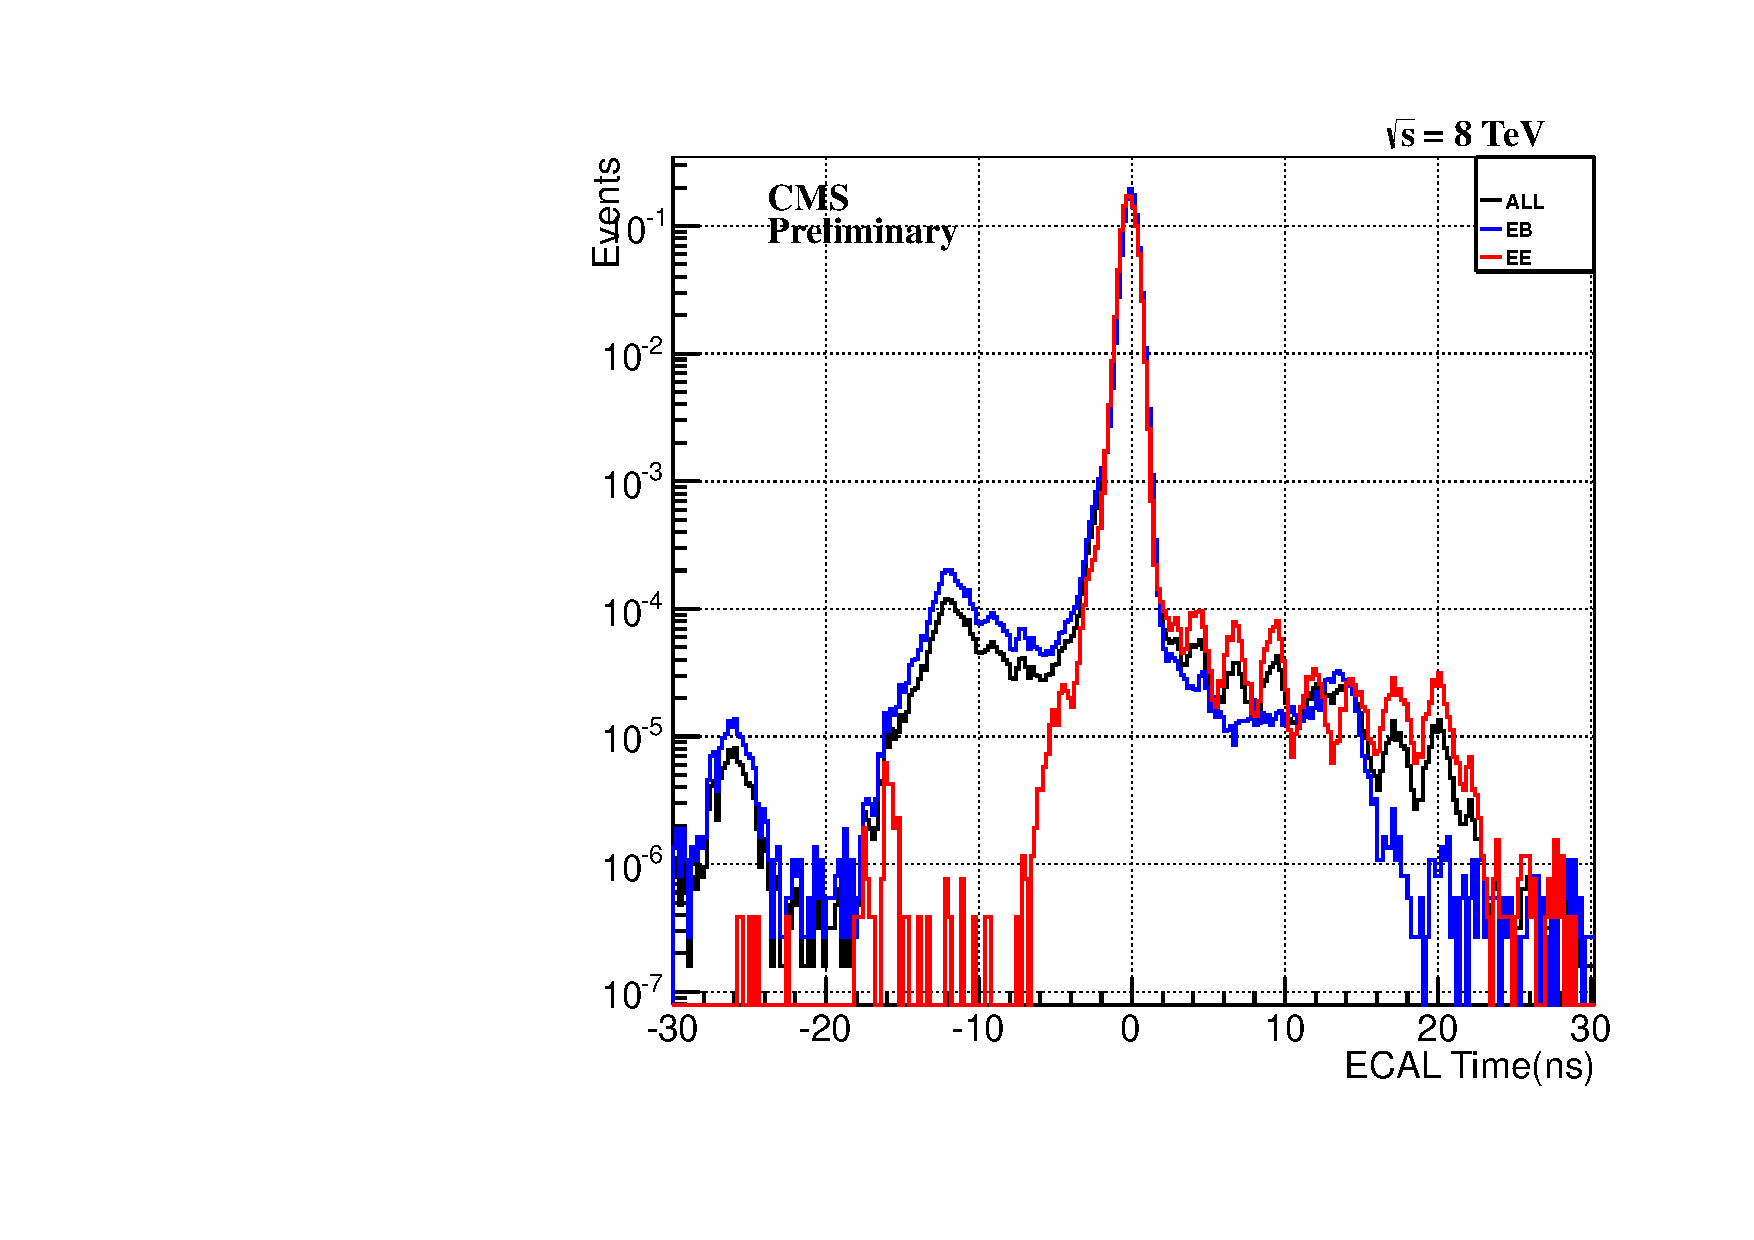
\includegraphics[height=0.65\textwidth, width=0.9\textwidth]{THESISPLOTS/Data-Photon-TimeEBEBALL.pdf}
}
\captionof{figure}{ECAL timing distribution of photons in barrel~(\textcolor{blue}{EB}), endcap~(\textcolor{red}{EE}) and all of ECAL~(\textcolor{black}{ALL ECAL}) with $\pt > 50$~GeV from data. A $2.5$~ns delay timing structure is observed in endcaps.}
\label{fig:TIMEECAL}
\end{center}
\end{minipage}

\vspace{5mm}
Most of the photons with this signature belong to the endcap~($1.47 < \eta < 3.0$) with a few in the barrel~($|\eta| < 1.47$). These out-of-time photons are produced  from beam halo muons from protons in \textit{Ghost}/\textit{Satellite} bunches or RF cavity, described in section \ref{Ghost}. We consider these events as background to our delayed photon signal. In addition to developing methods to tag and veto these events, a simple estimate of their contribution can be made using the ratio of the number of protons in the ghost RF cavities or bunches to the main proton bunches taken from the proton population in the RF cavity of the LHC proton filling profile. From this ratio, we estimate that one in every $100,000$ photons observed in ECAL particularly the endcaps, is from beam halo muons produced by ghosts bunches. Their presence is not clearly visible in the barrel as in the endcaps as they will be highly smeared in the barrel because their time is dependent on $\eta$ which is not the case in the endcaps. 
%is because very few of these photons are produced with high enough transverse momentum, \pt, to travel to the barrel and survive the 50\GeVc requirement. 
\newline
Our observation of this phenomenon together with the sub-par ECAL time resolution in the endcaps compared to the barrel, means, this analysis only uses photons belonging to the barrel.
\newline
We estimate, the contribution of these events to our delayed photon background in the signal using a  control sample of events with electromagnetic particles of moderate \pt range in the barrel like events with $\PZ \rightarrow \EE$ decay. The details of this study and the results obtained is discussed in the collision background estimation section of this analysis.
%%%
\subsection{\MET Adjustments}
  During energy clustering in the formation of superclusters used for event reconstruction by the particle flow~(PF) algorithm, "out-of-time" energy deposits in ECAL are excluded. The reason is because the algorithm avoids energy deposits from particles not produced from the main proton-proton bunch collisions like cosmic muons and machine induced backgrounds which are normally out-of-time. As a result of the exclusion, the out-of-time photon \et is not included in the calculation of missing transverse energy or \ETslash\hspace{0.15cm}~(from now on, we will be using for convenience, \ETslash\hspace{0.15cm} instead of \MET as the symbol for missing transverse energy) of the event. This exclusion introduces some differences in the calculation of \ETslash\hspace{0.15cm} for in-time~($|t_{\gamma}| < 3.0$~ns) and out-of-time photon events. 
\newline
Because energy deposits from events with out-of-time photons could be from a possible signal event, and we are searching for events with large arrival time photons, we correct for this exclusion by adding back the out-of-time photon's $\ET$ vector to the  particle flow reconstructed \ETslash\hspace{0.15cm}~(PF-MET) vector for events with out of time photons.
We introduced an additional missing transverse energy variable defined as $\vec{{\ETslash}^{\gamma}\hspace{0.15cm}} = \vec{\ETslash}\hspace{0.25cm} + \vec{\et}$, and use it in our final event selection to avoid any bias in our event selection, particularly for events with out-of-time photons. 
%%The difference between $\ETslash$\hspace{0.25cm} and ${\ETslash}^{\gamma}$ is given as
%%\begin{enumerate}
%%\item ${\ETslash}$~ : PF-MET equal to $\ETslash$\hspace{0.25cm} from standard event reconstruction.
%%\item ${\ETslash}^{\gamma}$~: PF-MET with photon \ET vector subtracted \ie ${\ETslash}^{\gamma} = \ETslash\quad - ~\et$ of the  out-of-time photon.
%% \end{enumerate}
%The distributions for ${\MET}_{1}$ and ${\MET}_{2}$  against ECAL time can be seen in figure \ref{fig:METS}.
%\begin{center}
%\centering
%\mbox{
%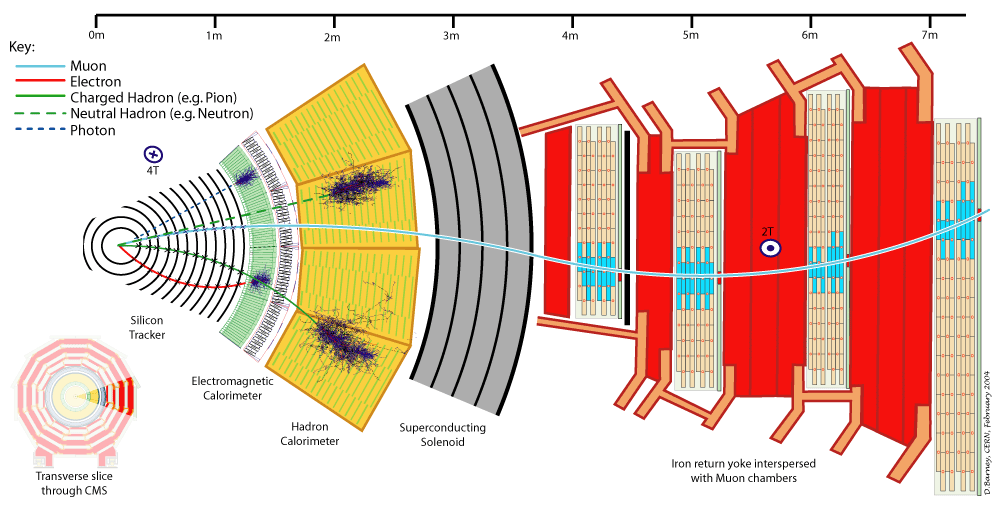
\includegraphics[scale=0.2]{THESISPLOTS/CMS_Slice.png}
%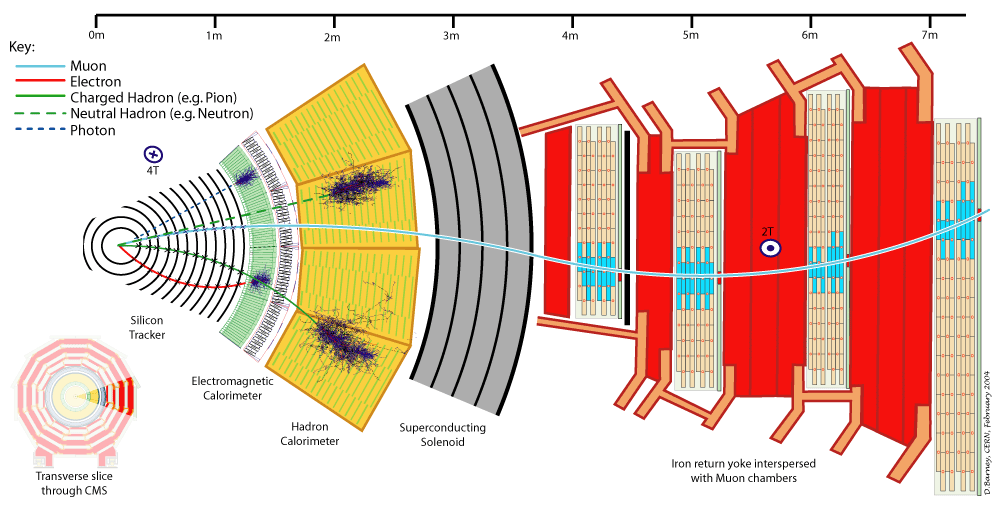
\includegraphics[scale=0.2]{THESISPLOTS/CMS_Slice.png}
%\captionof{figure}{Figure showing \MET distributions for events with out-of-time and in-time photons. ${\MET}_{1}$ and ${\MET}_{2}$ definitions are given in context. }
%\label{fig:METS}
%\end{center}
\section{Event Selection}
Our event selection happens in two stages. The first stage is online at the L1 and HLT trigger levels where only triggered single photon events are selected while the second stage happens offline where our signal-like event selection requirement is applied. 
\newline
The offline event selection criteria is designed to select signal-like events whose event topology comprise of at least a single photon, multiple jets and large \ETslash\hspace{0.15cm}. The multiple jets arise from the cascade decay of gluino or squark to other quarks/gluons in addition to the neutralino. We require multiple jets in our event selection as this helps suppress non-collision background events like cosmic and beam halo muons, and $pp$ collision background events like the ElectroWeak~(EWK) background events of $\PW \rightarrow e + \nu$ and $t\bar{t}$ decays, where the top~($t$) decays to a $b$ quark and a \PW boson 100\% of the time. These events with \PW boson can produce fake photons~(misidentified electron as photon) and real \ETslash\hspace{0.15cm} arising from the presence of the neutrino~($\nu$). 
\newline 
Other collision background events producing fake photons~(jet misidentified as photon) like multijets and QCD events can also be suppressed by selecting purely hadronic jets \ie jets containing a greater portion of hadronic energy fraction from pions and kaons.
\newline
The single late photon and large \ETslash\hspace{0.15cm} is from  $\PSneutralinoOne \rightarrow \gamma + \tilde{G}$ decay. We select only photons in the barrel~($|\eta_{\gamma}| < 1.479$). This suppresses out-of-time photons from the so-called halo muons from ghost/satellite proton bunches populating mostly the endcaps~($1.5 < \eta_{\gamma} < 3.0$). We also require the photons to be of high-\pt and this helps suppress misidentified out-of-time photon contribution from EWK events.
\newline
The large \ETslash\hspace{0.15cm} requirement is useful for suppressing $\gamma + $jets and QCD events with apparent \ETslash\hspace{0.15cm} or \textit{fake} \ETslash\hspace{0.15cm} which arise from energy misreconstruction and cracks in the detector. 
Out-of-time photon contribution from spikes can be reduced by applying electromagnetic shower shape selection on $S_{Minor}$ and $S_{Major}$ at the HLT trigger level. 
%%%
%%%
\subsection{Trigger Selection}
In our online event selection, we select events passing our online higher level trigger~(HLT): \texttt{HLT\_DisplacedPhoton65\_CaloIdVL\_IsoL\_PFMET25}, which is 
seeded by a level 1 trigger:\texttt{HLT\_L1SingleEG12}. The HLT trigger was developed primarily to trigger on events with delayed photons with the requirement  that the accepted event contains at least one photon with \pt more than 65\GeVc and \ETslash\hspace{0.15cm}~(without any out-of-time energy deposit bias) above 25\GeV. The minor axis of the photon electromagnetic shower must not be spread across many crystals in any direction. This is implemented as $ 0.1 < S_{Minor} < 0.4$ of the photon. We studied the HLT efficiency and turn-on~(efficiency becomes nearly 100\%) curve in the photon \pt and event \ETslash\hspace{0.15cm} and separately for \pt and \ETslash\hspace{0.15cm} using another trigger \texttt{HLT\_Photon50\_CaloIdVL\_IsoL} as the denominator. The \texttt{HLT\_Photon50\_CaloIdVL\_IsoL} selects photon candidates which are very loose isolated with $\pt > 65\GeVc$ and must also satisfy our offline photon selection requirement summarized in Table \ref{tab:PhotonSel}. The HLT event selection efficiency in \pt is defined as the fraction of offline reconstructed photons to photons triggered by the \texttt{HLT\_Photon50\_CaloIdVL\_IsoL} trigger within $\Delta R < 0.5$ while the efficiency in \ETslash\hspace{0.15cm} uses the \texttt{HLT\_Photon50\_CaloIdVL\_IsoL} trigger which has no \ETslash\hspace{0.15cm} and jet multiplicity requirement for the denominator and the \texttt{HLT\_DisplacedPhoton65\_CaloIdVL\_IsoL\_PFMET25} for the numerator
The results of the trigger efficiency measurements in photon \pt and event \ETslash\hspace{0.15cm} shown in Figure \ref{fig:HLTEff} indicate that the event selection efficiency is 100\% for events with photon $\pt > 80$\GeVc and $\ETslash\hspace{0.15cm} > 60$\GeV. %A \texttt{SinglePhoton} data sample is used to verify these efficiency study while the GMSB SPS8 and $\gamma +$jets samples are used to derive any correction factors between data and MC events.

\vspace{5mm}
\begin{minipage}{0.90\linewidth} 
\begin{center}
\mbox{
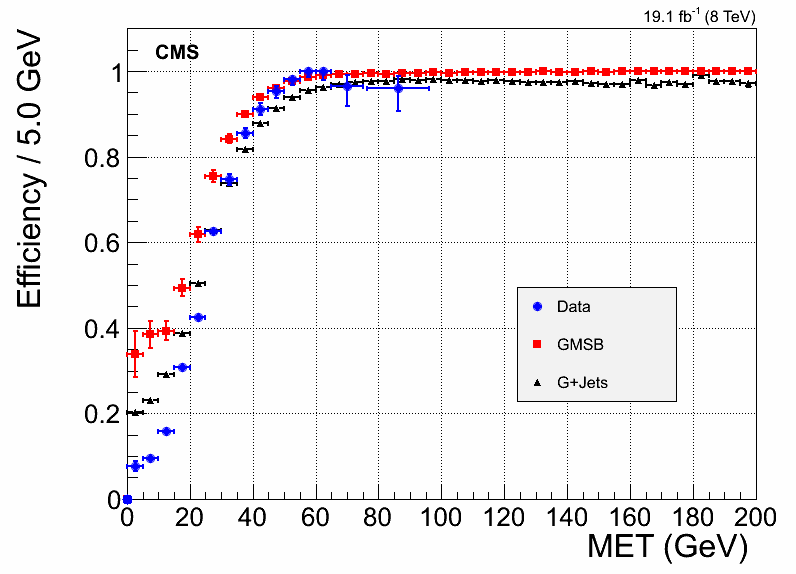
\includegraphics[height=0.45\textwidth, width=0.5\textwidth]{THESISPLOTS/PFMET_EffAsym.png}
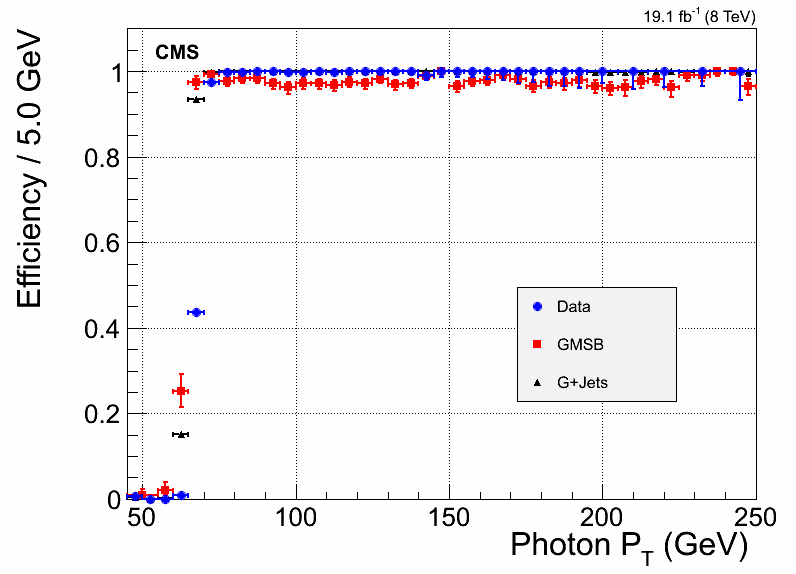
\includegraphics[height=0.45\textwidth, width=0.5\textwidth]{THESISPLOTS/Photon_EffAsym.png}}
\captionof{figure}{Our HLT trigger efficiency turn-on curves in photon \pt~(right) and event \ETslash\hspace{0.15cm}~(left).The $\gamma +$jets samples require photon $\pt > 170$~\GeVc.}
\label{fig:HLTEff}
\end{center}
\end{minipage}
%%%%
\subsection{Offline Selection}
Our offline event selection, applied on HLT triggered single photon events, require that the leading photon   have $\pt > 80\GeVc$ and if the event has more than one photon, the sub-leading photon have $\pt > 45\GeVc$. Electromagnetic showers initiated by charged hadrons are rejected by requiring $E^{\mbox{HCAL}}/E^{\gamma} < 0.05$, where $E^{\mbox{HCAL}}$ is the sum of the energy in the HCAL towers directly behind the ECAL photon supercluster within a $\Delta R < 0.15$, with $\Delta R = \sqrt{(\eta - \eta^{\gamma})^{2} + (\phi - \phi^{\gamma})^{2}} $, and $E^{\gamma}$ the photon energy in ECAL. Electrons are rejected by requiring the absence of hits in the first two layers of the pixel detector that is consistent with an electron track matching the observed location and energy of the photon candidate~(this is known as pixel veto requirement).
\newline
The photon candidates must satisfy three \textit{isolation} requirements that reject photons produced in hadronic decays:(1) $Iso_{\mbox{TRK}} < 0.2\GeV$, where $Iso_{\mbox{TRK}}$ is the sum of the \pt of tracks compatible with the primary event vertex in an annulus $0.015 < \Delta R < 0.40$, excluding a strip half $\eta$ width of 0.015 and the additional inner cone of size 0.04, optimized to exclude reconstructed tracks from $\PZ\rightarrow \EE$ events, centered around the line of vertex pointing to the photon supercluster. The exclusion is to remove the photon's own energy if it converts into an $\EE$ pair;
(2) $Iso_{\mbox{ECAL}} < 4.5\GeV$, where $Iso_{\mbox{ECAL}}$ is the transverse energy deposited in ECAL in an annulus  $0.045 < \Delta R < 0.4$ centered around the photon ECAL supercluster, excluding the strip half $\eta$ width of 0.02 and the additional inner cone of size 0.045 centered around the ECAL supercluster position; (3) $Iso_{\mbox{HCAL}} < 4.0\GeV$, where  $Iso_{\mbox{HCAL}}$ is the transverse energy of HCAL tower in an annulus of $0.15 < \Delta R < 0.40$ centered about the ECAL supercluster position.
If the photon is very closed to a track within a range in $\Delta R(\gamma, track) < 0.6$ it is rejected. This is to avoid misidentifying charge particles as photons and to prevent double counting jets with high electromagnetic energy component as photons. The photon must also be isolated from any other particle in a cone size of $\Delta R(\gamma, \mbox{particle})< 0.4$.  The size of the photon electromagnetic shower along the minor axis~($S_{Minor}$) must be be within 0.12 and 0.38 to suppress photons embedded in hadronic jets. 
\newline
Only photons belonging to the barrel~(EB) region \ie $|\eta_{\gamma}| < 1.479$, are accepted to avoid many out-of-time photon candidates from ghost/satellite beam halo which belong to the endcap~(EE) shown in Figure \ref{fig:TIMEECAL}.
\newline
Topological selection cuts, $1 - E_{6}/E_{2} < 0.98$ and $ 1 - E_{4}/E_{1} < 0.98$ on the photon energy deposit helps suppress direct interactions in the ECAL APDs by charged particles and neutrons producing anomalous photons known as spikes.
Our full photon selection criteria is presented in Table \ref{tab:PhotonSel}.
\newline
For jets, we select jets with $\eta_{jet} < 2.4$, require that the leading jet in the event has a $\pt > 35\GeVc$ and the number of jets in an event must be at least 1. This helps suppress non-collision background events without jets. The jets are reconstructed using the PF algorithm and identified based on the  identification selection criteria summarized in Table \ref{tab:JetSel}, where the charge electromagnetic fraction~(CHF) and the neutral electromagnetic fractions~(NEF) must make up a greater portion of the jet sub-structure~($>99$\%),the neutral energy fraction~(NEF) must be than 99\% less in order that the jet is not easily misidentified as a photon. A jet near a photon object within a cone of 0.3 is rejected. 
\newline
From our HLT trigger event selection efficiency plot in Missing Transverse Energy~(MET) shown in Figure \ref{fig:HLTEff}, we observed that a missing transverse energy of at least 60\GeV for \ETslash\hspace{0.15cm} and ${\ETslash}^{\gamma}\hspace{0.15cm}$ is enough to suppress $\gamma + $jets and QCD events with apparent missing transverse energy.


\vspace{5mm}
\begin{minipage}{0.85\linewidth} 
\begin{center}
%\begin{table}[ht]
\begin{tabular}{l c }
\toprule
\hline
\multicolumn{2}{l}{\bfseries{Photon Selection Criteria}} \\
  \hline 
  \bfseries{Criteria} & \bfseries{Requirement} \\
   \hline 
   \toprule
 % \texttt{primary vertex number of tracks(vnof)}& $>= 4$ \\
 % \texttt{primary vertex transverse distance to beam}~($d0$) & $ < 2$~cm from CMS center \\
%  \texttt{primary vertex longitudinal distance to beam}~($|z|$) & $ < 24$~cm from CMS center \\
  \texttt{Event leading photon must have} $\pt(\gamma^{1})$  & $ > 80$~ GeV \\
  \texttt{Other photons in event must have} $\pt(\gamma^{2,3,...})$  & $ > 45$~ GeV \\
 $|\eta_{\gamma}|$,(\texttt{Barrel Only}),  & $ < 3.0$ ($ < 1.5$) \\
 $S_{Minor}$  & $ 0.12 \leq S_{Minor} \leq 0.38$ \\
 $E^{\mbox{HCAL}}/E^{\gamma}$  & $ < 0.05$ \\
 $\Delta R(\gamma, track)$  & $ > 0.6 $ \\
 $Iso_{\mbox{HCAL}}$, $Iso_{\mbox{ECAL}}$, $Iso_{\mbox{TRK}}$  & $ < 4.0\GeV $, $ < 4.5\GeV $, $ < 0.2\GeV $ \\
 Photon Isolation cone size $\Delta R(\gamma, \mbox{particle})$ & $< 0.4$ \\
 Topological Spike cuts  & $1 - E_{6}/E_{2} < 0.98$, $ 1 - E_{4}/E_{1} < 0.98$ \\ 
  \hline 
  \bottomrule
\end{tabular}
\captionof{table}{The photon identification and selection  criteria used in this analysis}
\label{tab:PhotonSel}
%\end{table}
\end{center}
\end{minipage}

\vspace{5mm}
\begin{minipage}{0.85\linewidth} 
\begin{center}
%\begin{table}[ht]
\begin{tabular}{l c }
\toprule
\hline
\multicolumn{2}{l}{\bfseries{Jet PF identification selection criteria}} \\
  \hline 
  \bfseries{Criteria} & \bfseries{Requirement} \\
   \hline  
   \toprule
\texttt{Jet} \pt & $ > 35$\GeV \\
 \texttt{Number of Jet constituents} & $ > 1$ \\
 \texttt{Charge EM energy fraction~(CEF) } & $ > 0.99$ \\
 \texttt{Neutral Hadron energy fraction~(NHF) } & $ < 0.99$ \\
 \texttt{Neutral EM energy fraction~(NEF) } & $ < 0.99$ \\
 \texttt{If} $|\eta|$ \texttt{of jet is} $ >2.4$, \texttt{Charge Hadron energy fraction~(CHF) } & $ > 0$ \\
 \texttt{If} $|\eta|$ \texttt{of jet is} $ >2.4$, \texttt{Charge multiplicity~(NCH) } & $ > 0$ \\
 $\Delta R(\gamma, jet) = \sqrt{(\phi_{\gamma}-\phi_{jet})^{2} + (\eta_{\gamma}-\eta_{jet})^{2}}$ & $ > 0.3$ \\
 \toprule
 \texttt{\ETslash \hspace{0.25cm}, ${\ETslash}^{\gamma}\hspace{0.15cm}$} & $ > 60\GeV$ \\
\hline
\bottomrule
\end{tabular}
\captionof{table}{The Jet ID and MET selection used in this analysis}
\label{tab:JetSel}
%\end{table}
\end{center}
\end{minipage}

\vspace{5mm}
\begin{minipage}{\linewidth} 
\begin{center}
\centering
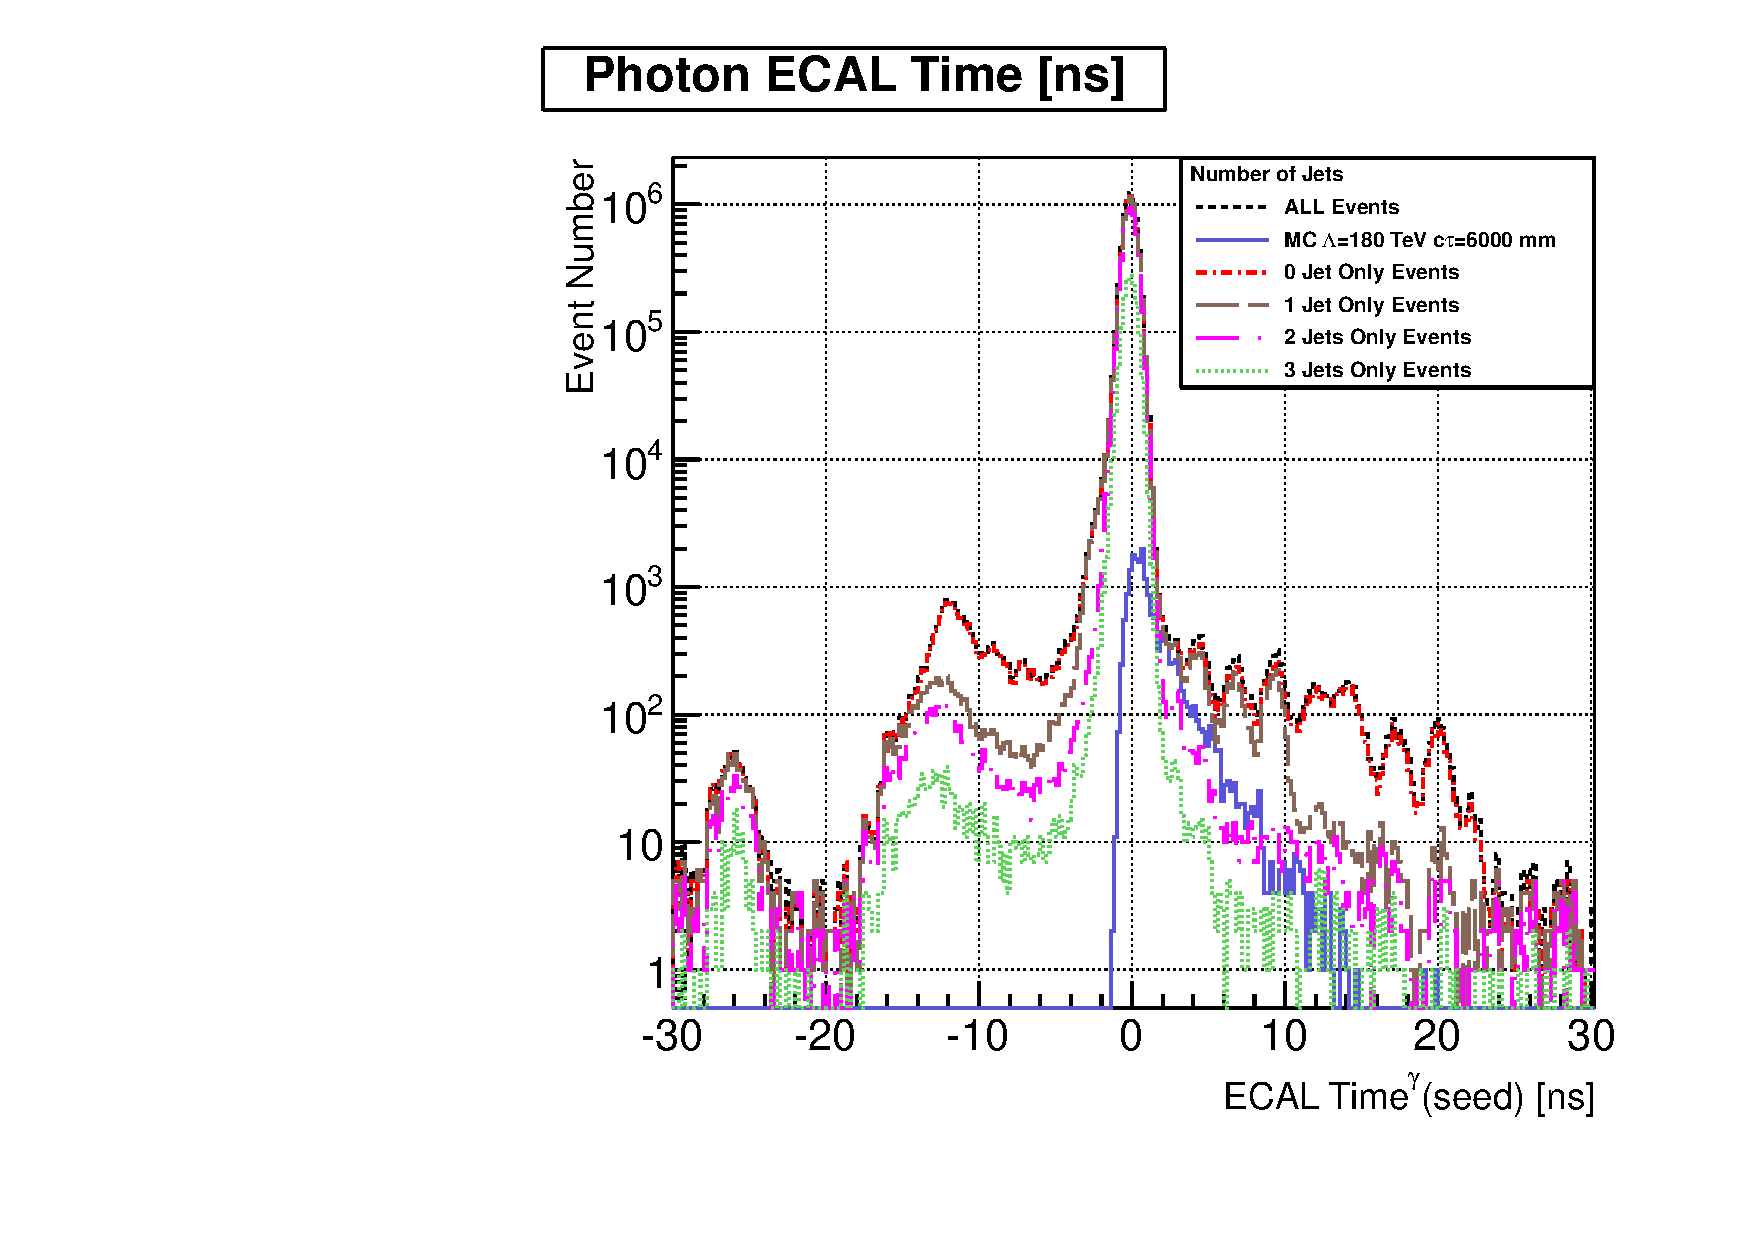
\includegraphics[height=0.65\textwidth, width=0.8\textwidth]{THESISPLOTS/Photon_SeedXtalTime_Distribution_VsJetMultiplicity.pdf}
\captionof{figure}{Comparing ECAL time distribution of events with different jet multiplicity from small sample of data and a single GMSB $\Lambda=180\TeV$ and $c\tau=6000$~mm sample. Accepted photons must have $\pt > 60$\GeV.}
\label{fig:TimePlotJet}
\end{center}
\end{minipage}

\vspace{5mm}
\par
  In summary, our signal events are events whose topology comprise of $\ge1~\gamma + \ge2~ jets + \ETslash\hspace{0.15cm} > 60\GeV + {\ETslash}^{\gamma}\hspace{0.15cm} > 60\GeV$. In Figure \ref{fig:TimePlotJet}, we observed that most of our background events, especially non-collision background events like beam halo, are mostly zero and one jet events. Thus, we use these zero and one jet events as a control sample to do our background study.

%%%$$$

\section{Background Estimation}
Most of our background events with out-of-time photons are non-collision events produced from many different sources. In order to qualify and quantify the different sources, we compare in-time~($|t_{\gamma}| < 2$~ns) photon candidates to out-of-time~($t_{\gamma} < -3$~ns and $t_{\gamma} > 3$~ns) photon candidates.
By also comparing photon candidates of events with different number of jets, we were able to uncover the different background sources and better quantify their contribution. In Figure \ref{fig:BKGPLOTS}, we present scatter plots of the photon's ECAL time against $\eta$~(left) and against $\phi$~(right) for events with photon $\pt < 60\GeV$, belonging to both the barrel and endcap regions and event $\ETslash\hspace{0.15cm} > 25\GeV$.

\vspace{5mm}
\begin{minipage}{0.90\linewidth} 
\begin{center}
\centering
\mbox{
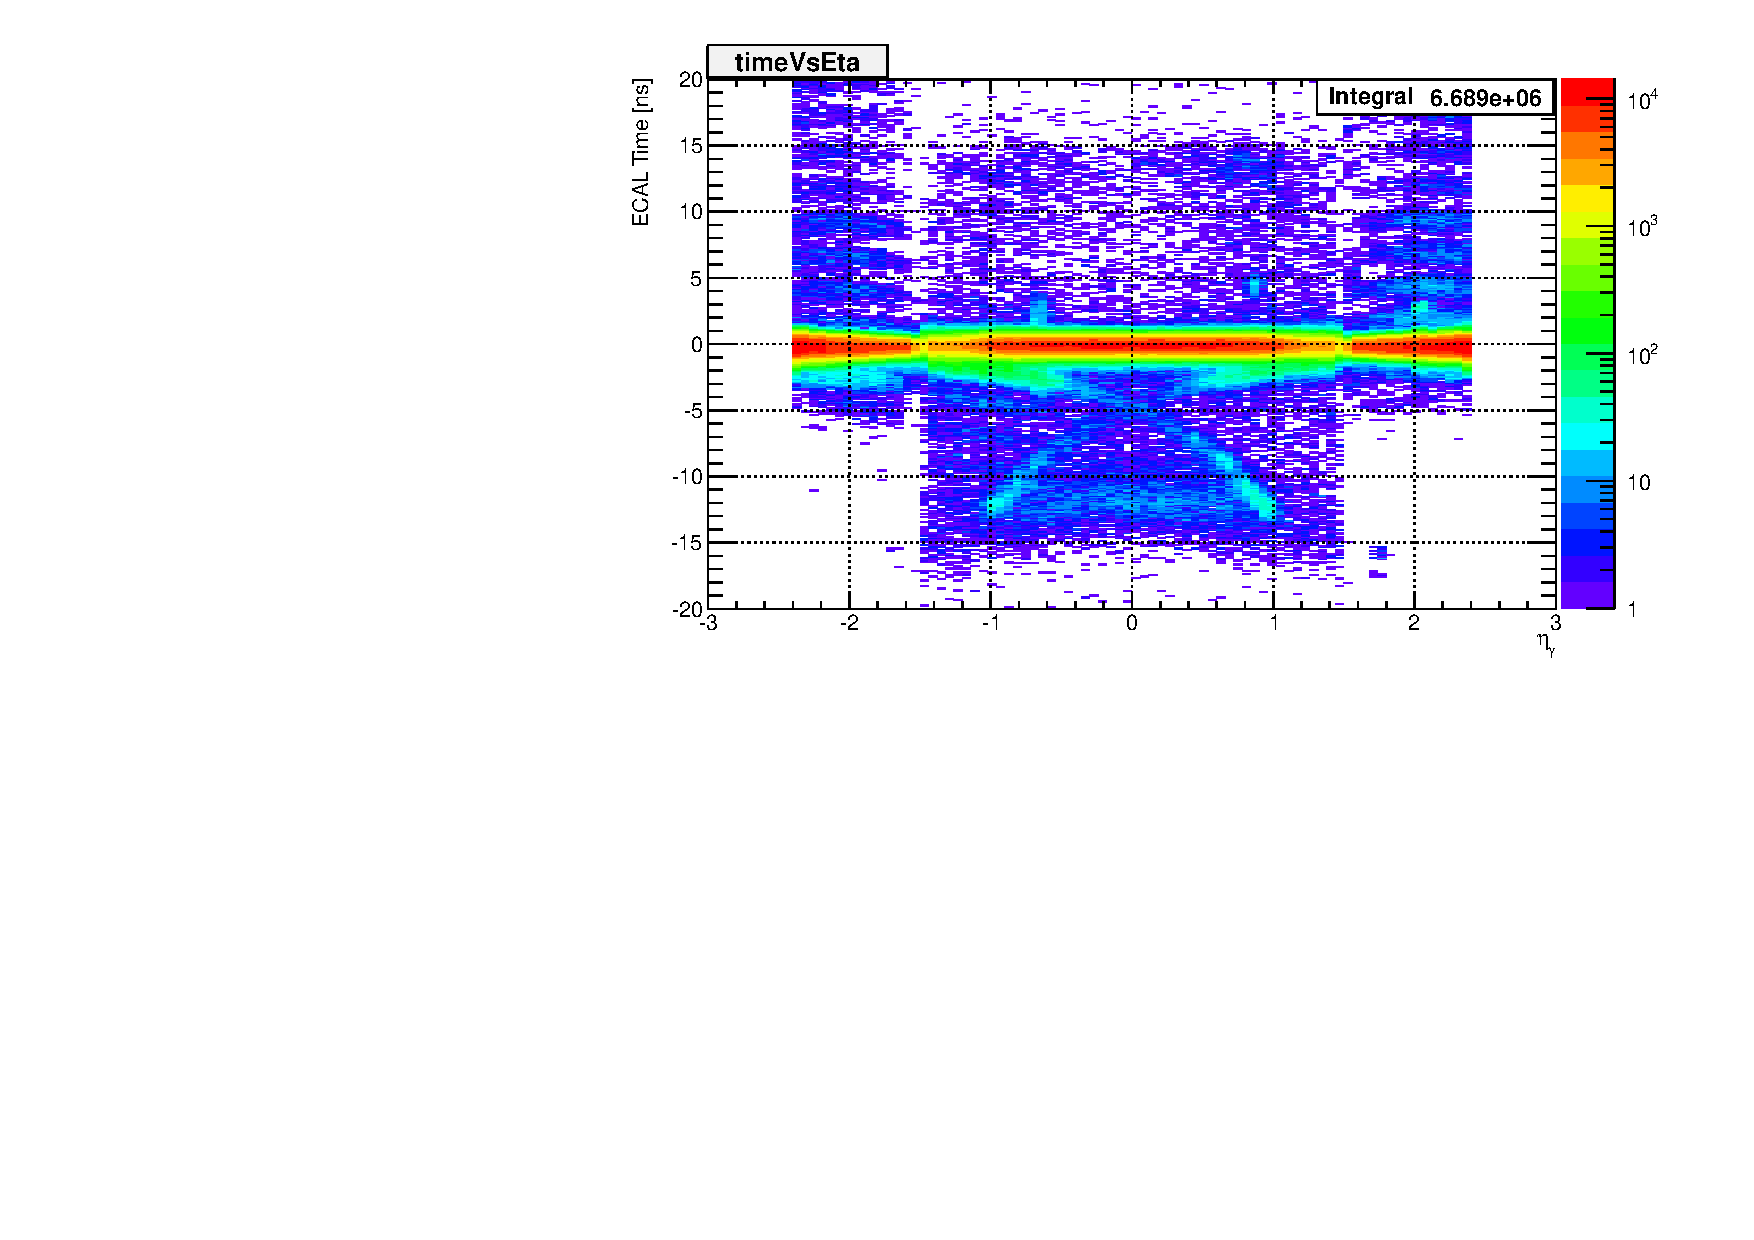
\includegraphics[height=0.4\textwidth, width=0.5\textwidth]{THESISPLOTS/SinglePhotonDataSet-TimeVsEta.pdf}
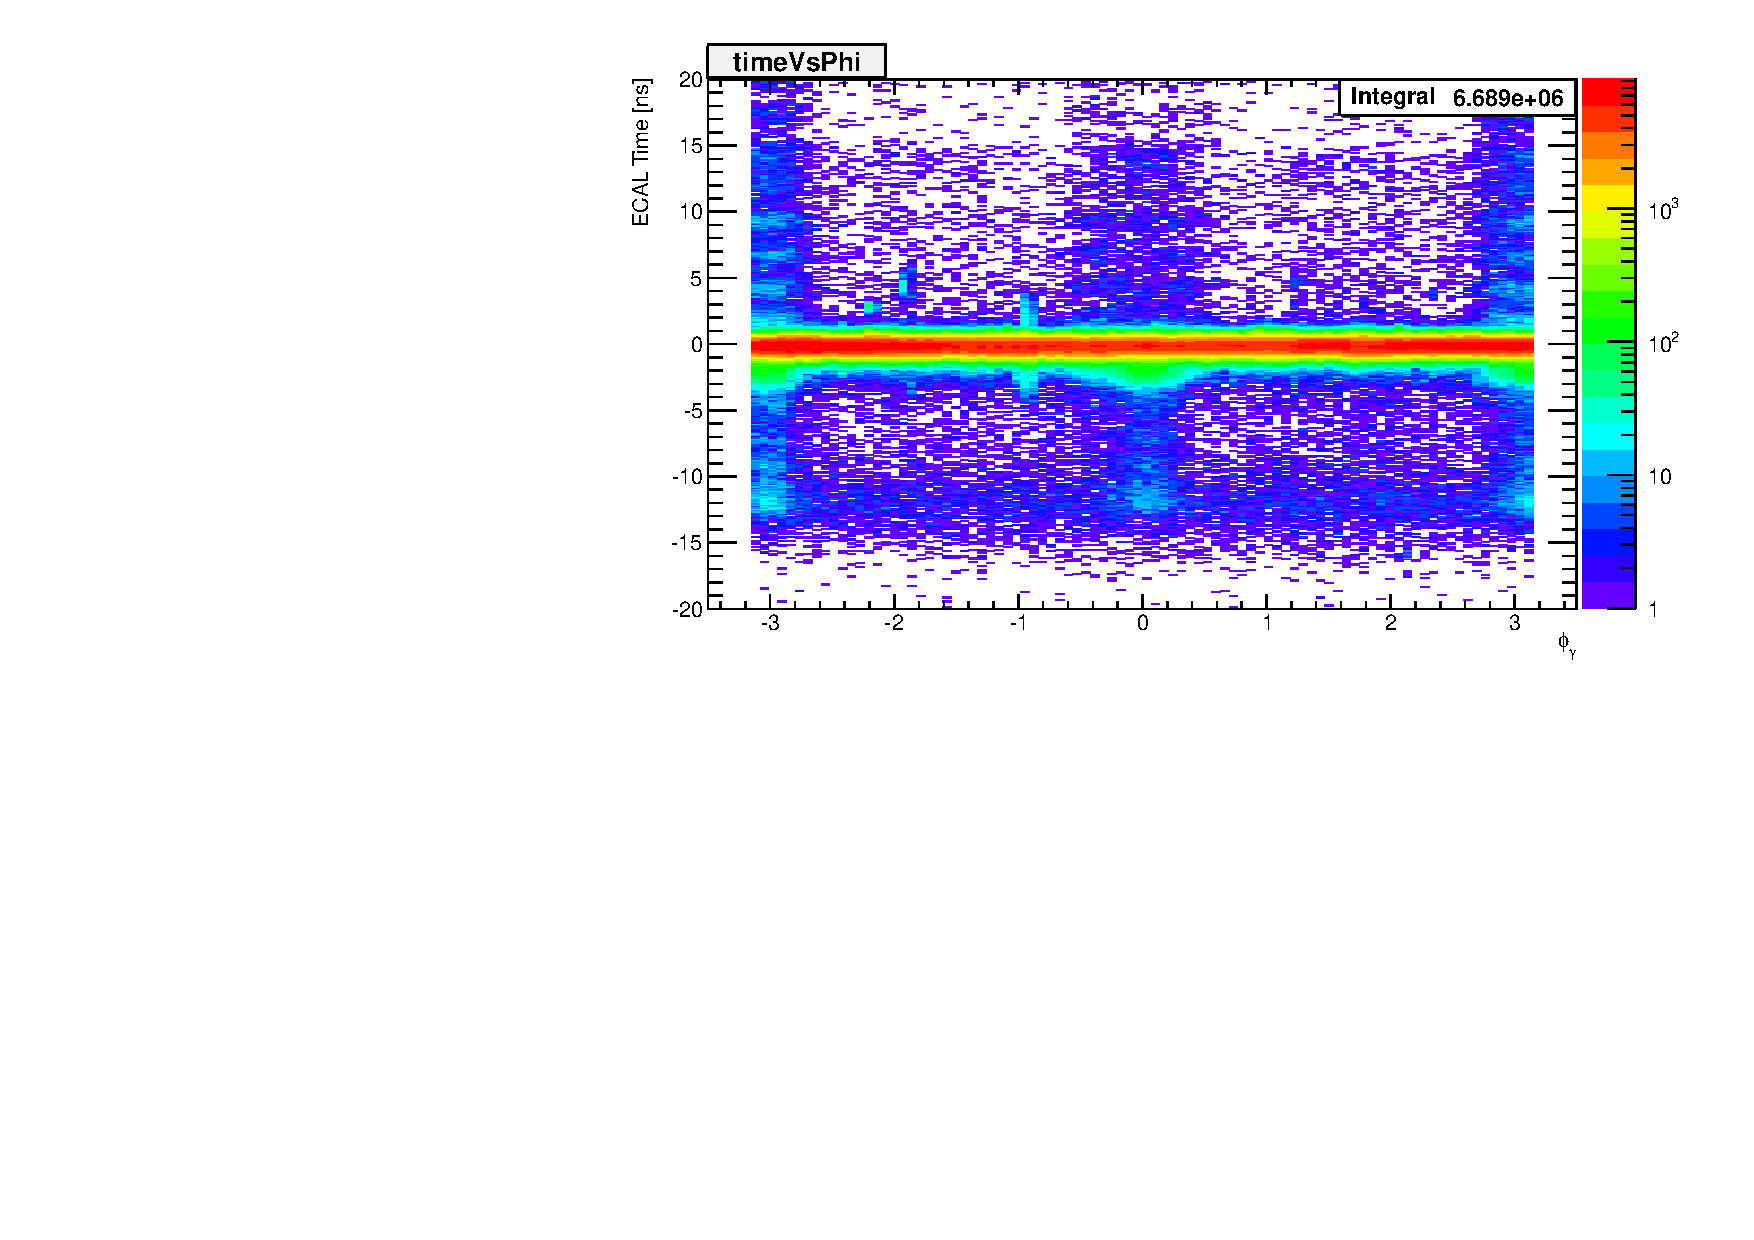
\includegraphics[height=0.4\textwidth, width=0.5\textwidth]{THESISPLOTS/SinglePhotonDataSet-TimeVsPhi.pdf}}
\captionof{figure}{ECAL time against $\eta$~(left) and ECAL time against $\phi$~(right) for photons with $\pt > 60$\GeV from data.}
\label{fig:BKGPLOTS}
\end{center}
\end{minipage}

\vspace{5mm}
From these plots, we observe that, although most of the photons arrive with ECAL time about zero, a good number of photons are out-of-time and from very different sources, for example, the cross-like feature seen in the plot on the left, is particular to photons with earlier ECAL time while the step-like pattern in ECAL time extends to all out-of-time photons but is more prominent to photons which belong to the endcap regions~($1.479 < \eta_{\gamma} < 3$) and have late ECAL time. The high concentration of out-of-time photons at $\phi=0\pm\pi$ on the right plot indicate a unique source of non-collision events which is not random. We conclude that the possible sources of background photon candidates with out-of-time can be split into photons from beam halo muons, because of the cross-like feature and high population at $\pi=0\pm\pi$, cosmic muons, due to the random distribution of out-of-time photons throughout ECAL and spikes, due to the high concentration of photons with ECAL time of about -12.5~ns. The step-like feature can be attributed to photons arising from ghost/satellite bunch collisions while a small contribution of out-of-time photons is from QCD  and electroweak events. To reduce the contamination of possible signal out-of-time photons from spikes which contribute the most to events with out-of-time photons particularly with ECAL time around $t_{\gamma} \approx -12$~ns, we restrict our event selection to photons with ECAL time $ 2.0 < t_{\gamma} < 13.0$~ns and $-10.0 < t_{\gamma} < -3$~ns, making our search restricted to signal events with photon ECAL time between $2.0 < t_{\gamma} < 13.0$~ns.
\newline
For our background estimation study, we split the background events into two categories: Collision and Non-Collision events. We first identify and reject photon candidates from beam halo, cosmic muons and spikes and then estimate the residual non-collision and collision background photon candidates  using the \textbf{\textsf{ABCD}} background estimation technique. 

\subsection{Collision Background}
\subsubsection{QCD Photons}
Events from satellite/ghost proton bunches described in section \ref{Ghost}, produce out-of-time photons which can be present in the barrel. Because these photons are produced from collisions just like QCD events, we refer to these photons as QCD photons. It is challenging to define a strategy for rejecting this background events. Our approach, after rejecting non-collsiion events, is to estimate their contribution to signal using the \textsf{ABCD} background estimation method. We also perform a separate background estimation using a control sample of \PZ events, and show that background contributions from events with QCD photon candidates from satellite/ghost is almost negligible.% We elaborate more on this in the collision background estimation section.%We will More on this is discussed in future sections.
%%%%
\subsection{Non-Collision Background}
%We study non-collision background events from beam halo muons, cosmic muons, and spikes using a data sample of zero and one jet events passing all our event selection requirements.
% These events consist of have photons with large reconstructed time and large \ETslash\hspace{0.15cm} measurements. The high \pt photons from these energetic muons and possible overlapping  pile up events from multiple $pp$ collisions, contribute to the total sum of the PF reconstructed \pt imbalance leading to their large \ETslash\hspace{0.15cm} and at times jets associated with these events.
%We select events with at least one good vertex, zero or one jet, photons satisfying ECAL spike cleaning, associated with candidate muons satisfying DT time cosmic muon cleaning and CSC tight halo-muon cleaning requirements to study these non-collision events. 
%A schematic diagram in Figure \ref{fig:NeutDecay} show the production of photons from both non-collision and collision{ghost/satellite} in a typical LHC $pp$ collision within the CMS detector. Also shown is a typical photon from a neutralino decay in the GMSB model. Still on the diagram is shown the point of entry of beam halo muons into the CMS detector comparing to what is observed in the photon ECAl time against $\eta$ and $\phi$ plots of Figure \ref{fig:BKGPLOTS}.

%\vspace{5mm}
%\begin{minipage}{0.90\linewidth} 
%\begin{center}
%\captionsetup{type=figure}
%\mbox{
%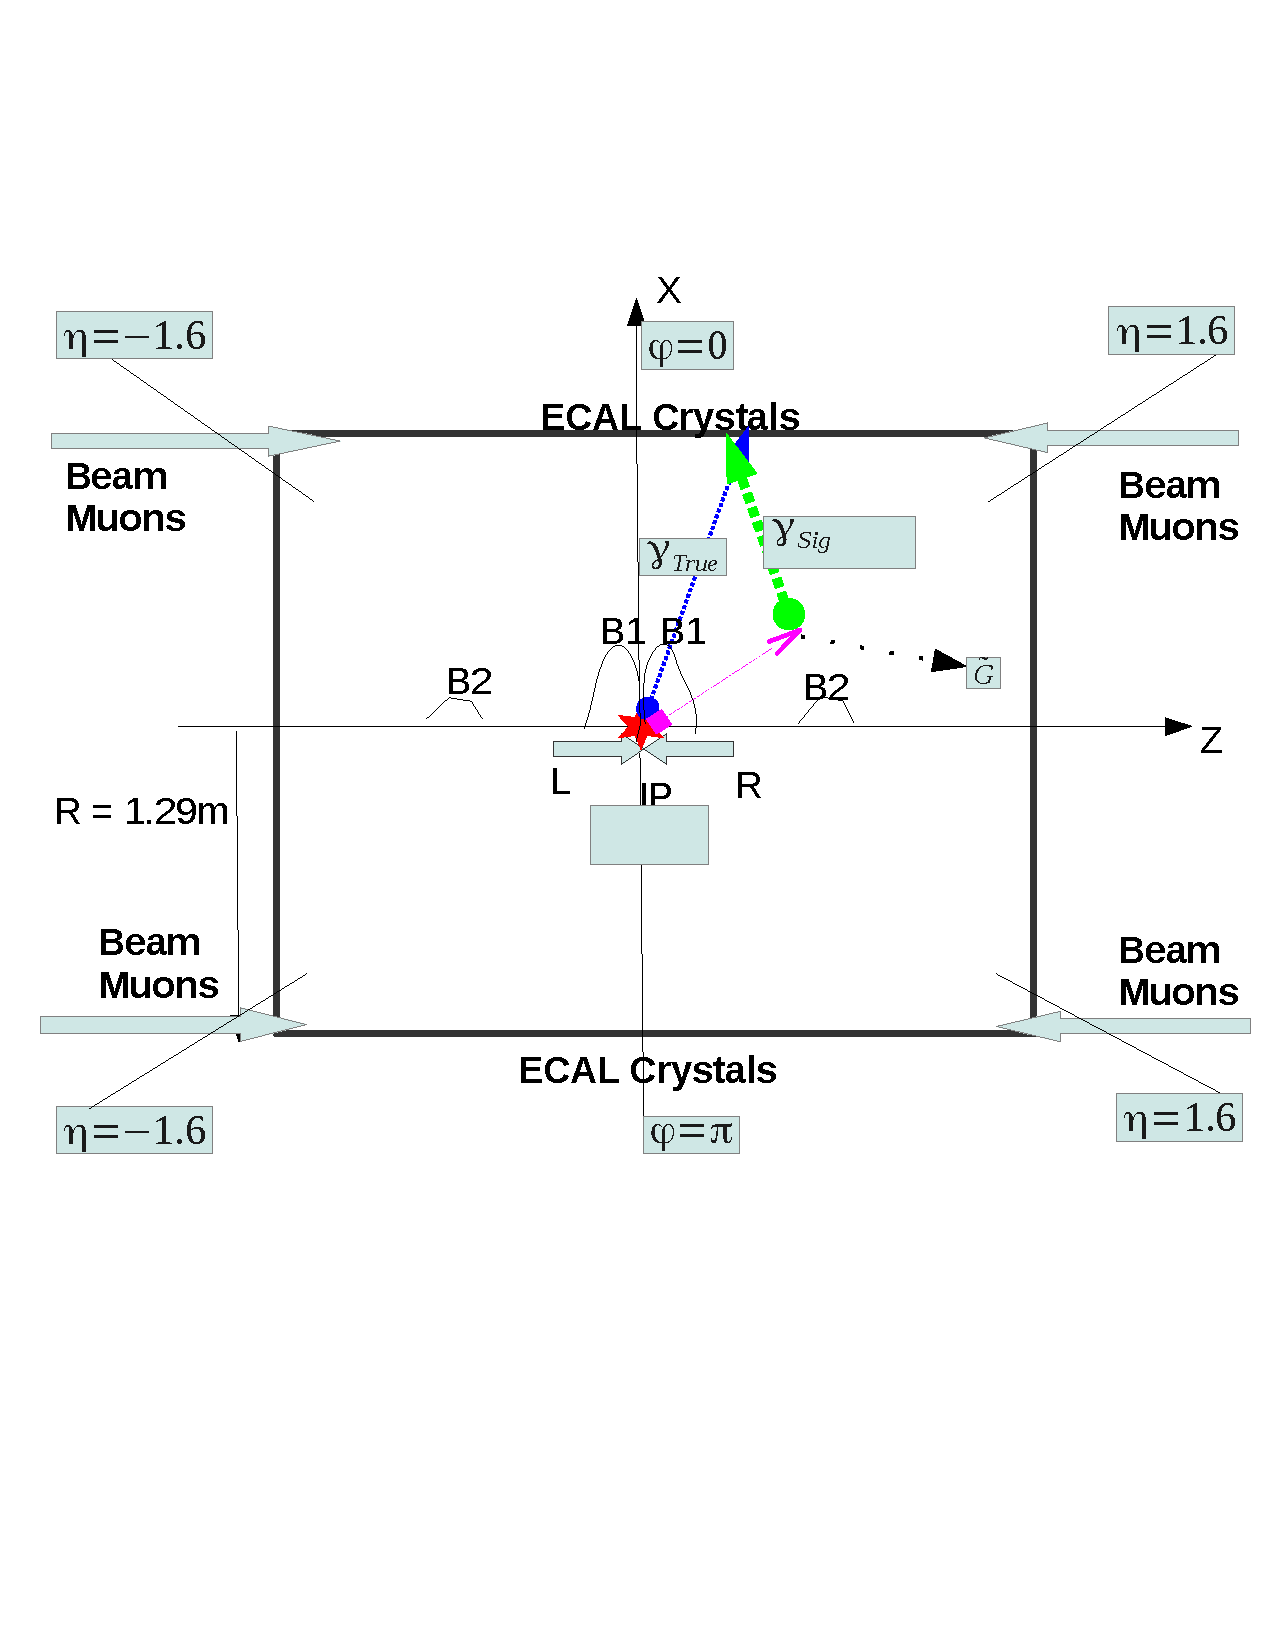
\includegraphics[height=0.35\textwidth, width=0.5\textwidth]{THESISPLOTS/Background_Delayed_Photon.pdf}}
%\captionof{figure}{Schematic diagram showing production of photons from main $pp$ and possible ghost/satellite bunch collisions in the CMS detector volume. Typical beam halo muon's entry direction into ECAL and GMSB neutralino decay is shown.}
%\label{fig:NeutDecay}
%\end{center}
%\end{minipage} 
%%%%%

\subsubsection{Halo Photons}
Protons in the main and sometimes ghost/satellite bunches can, through inelastic scattering with residual gas molecules like $\mbox{H}_{2}$ and C$\mbox{O}_{2}$ in beam pipe, produce pions which later decay into muons called \textit{Beam Halo} muons, traveling with energy of about a few \TeV. These energetic muons radiate energetic photons called \textit{Halo photons} in the calorimeter through a process called \textit{bremsstrahlung}. It is also possible that beam halo muons can be produced when protons scatter off Tertiary Collimators~(TCT), due to proton beam deflection by the magnets, just before entering the CMS detector.
The halo muons can travel nearly parallel to the main proton bunch but often stir away from the nominal orbit in the transverse direction spreading mostly in the horizontal plane, with respect to the CMS detector coordinates, due to betatron oscillations. Despite beam cleaning, a sizable population of beam halo muons remains eventually producing energetic photons in the calorimeters. A scatter plot of the photon ECAL time against $\phi$  shown earlier in the right plot of Figure \ref{fig:BKGPLOTS}, show that most of these beam halo muons enter the ECAL in the horizontal plane at $\phi=0,\pm\pi$. The rate of halo photons in the general proton \textit{Beam-Induced Background}~(BIB) events depend on the beam current and the operational conditions of the LHC like the  machine optics, collimator settings, residual gas densities and RF cavity filling scheme. 
\newline
The halo muons before entry into ECAL, produce hits which can be reconstructed into muon tracks using segments in the Cathode Strip Chambers~(CSC) Endcap muon detectors. The reconstructed hits in the CSC segments can be associated with a halo photon supercluster in ECAL within some narrow opening angle in $\phi$. The geometry of ECAL allows most of the halo muons in the endcaps but also enough in the barrel. The resulting halo photons are usually out-of-time compared to photons produced directly from nominal $pp$ collisions and most of them have earlier arrival time in cases where the beam halo muons arrive at the ECAL crystals before $pp$ collisions occur at the interaction point. This arrival time can be estimated from the unique flight path of the beam halo muons with respect to the arrival time of photons from $pp$ collisions as 
\begin{equation}{\label{eq:HALOPATH}}
t^{\mbox{expected}}_{\mbox{ECAL}} = -1/c\left( \pm Z_{\mbox{cluster}} + \sqrt{Z^{2}_{\mbox{cluster}} + R^{2}_{\mbox{cluster}}}  \right),
\end{equation}
where $Z_{\mbox{cluster}}$ is the point where the halo muon hits ECAL or longitudinal distance along $z$-axis of the halo photon supercluster position from the nominal interaction point, $R$ is the radial distance of the supercluster from the beam line which is the radius of ECAL equal to $1.29$\m and $c$ is the speed of light in vacuum. The estimated halo muon ECAL arrival time can be re-arrange to become
\begin{equation}{\label{eq:HALOPATH2}}
t^{\mbox{expected}}_{\mbox{ECAL}} = - \frac{R}{2c} \exp^{(-\eta)}
\end{equation} 
showing the explicit dependence on $\eta$, for the beam halo muon entry point in ECAL. Comparing this estimated time shown in Figure \ref{fig:HALO} as the two red lines, with observation from data for the 2-dimensional plot of ECAL time $vs$ $\eta$ of photon candidates, show a nice agreement especially for earlier arrival time photon candidates.

\par
By matching halo muon hit positions in CSC segments to photon supercluster positions in the ECAL calorimeter in $\phi$, since halo muons spread mostly in the horizontal plane or azimuthal~($\phi$) direction, we are able to match halo muons to their corresponding halo photons. We use the quantity, $\Delta\phi(\mbox{CSC Seg},\gamma)$, which is the difference in $\phi$ between the CSC segment  and the photon supercluster position in ECAL, to express this matching. A plot of $\Delta\phi(\mbox{CSC Seg},\gamma)$ for in-time and out-of-time photons is shown in the left plot of Figure \ref{fig:HALO}. We see that out-of-time photons have small $\Delta\phi(\mbox{CSC Seg},\gamma)$ confirming that some out-of-time photons are produced by beam halo muons.

\vspace{5mm}
\begin{minipage}{0.90\linewidth}  
\begin{center}
%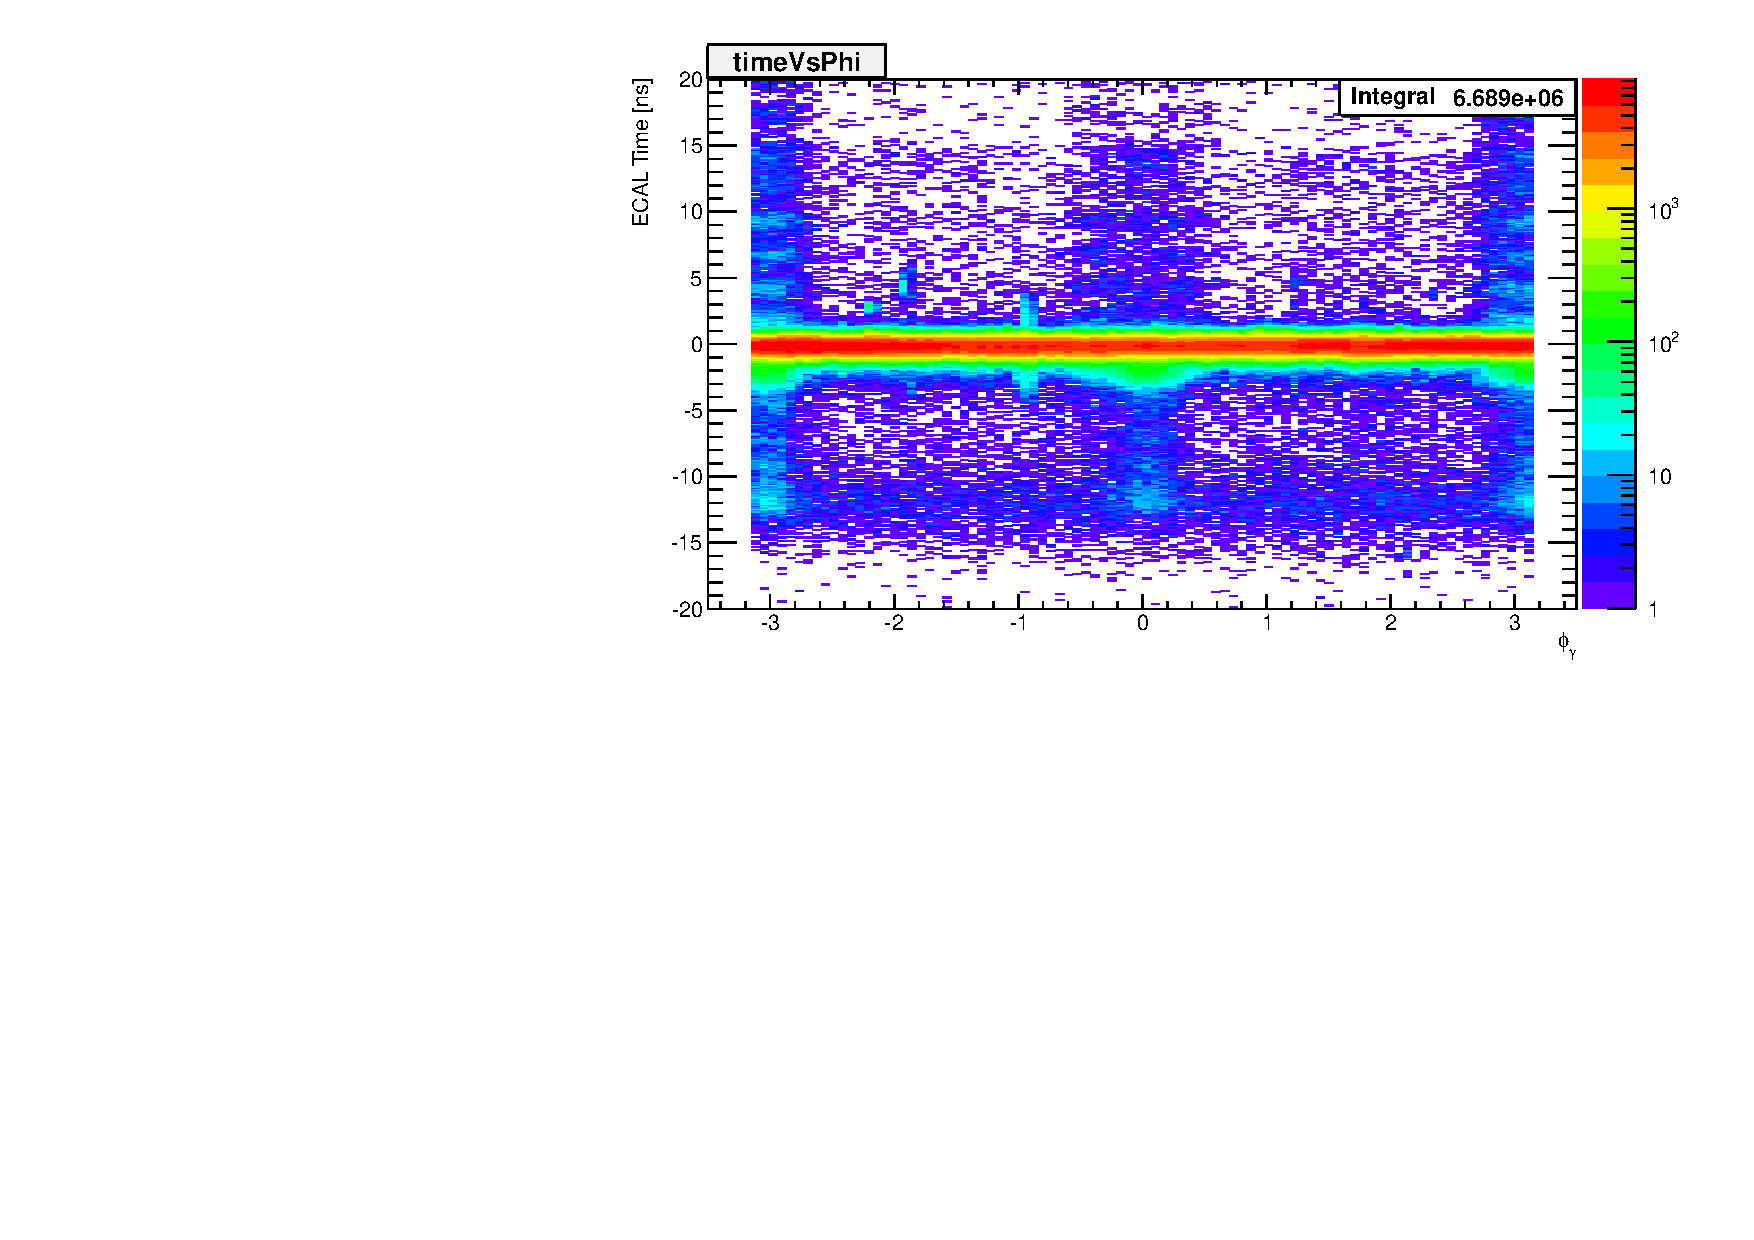
\includegraphics[height=0.35\textwidth, width=0.5\textwidth]{THESISPLOTS/SinglePhotonDataSet-TimeVsPhi.pdf}}
\mbox{
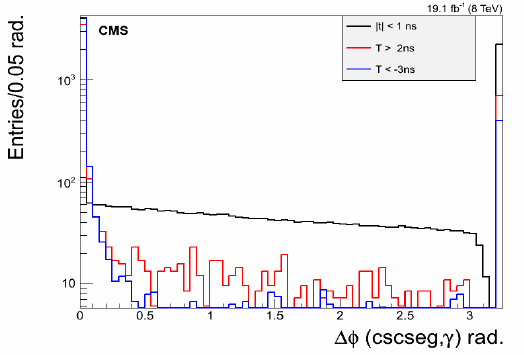
\includegraphics[height=0.45\textwidth, width=0.5\textwidth]{THESISPLOTS/CSC-Segment-Halo-Tagging.png}
%{THESISPLOTS/CSC_Segment_Halo_data.png}
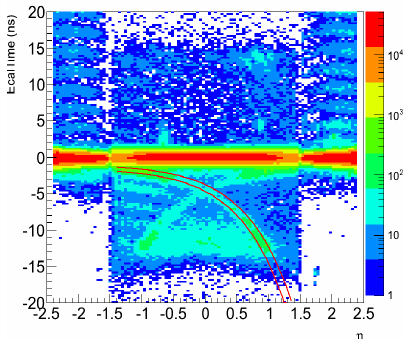
\includegraphics[height=0.45\textwidth, width=0.5\textwidth]{THESISPLOTS/HALO-ECAL-TIME-Vs-ETA.png}}
\captionof{figure}{(Left) ECAL time $V.s$ $\Delta\phi(\mbox{CSC Seg},\gamma)$ for in time(black) and out-of-time(red and blue) photons. (Right)Photon ECAL time $V.s$ $\eta$, expected halo photon time is shown as two red lines.}
\label{fig:HALO}
\end{center}
\end{minipage}

\vspace{5mm}
To estimate the performance of using $\Delta\phi(\mbox{CSC Seg},\gamma)$ for tagging events with halo photons, we use a halo photon candidate sample of selected events with photons in the endcaps where we expect mostly halo photon candidates and with $\phi_{\gamma}$ around $\phi = 0, \pm \pi$. We were able to tag with $\Delta\phi(\mbox{CSC Seg},\gamma) < 0.05$, a good number of photon candidates as halo photons in the endcaps shown in the Figure \ref{fig:HALOENDCAP} comparing halo photons in the endcaps to tagged halo photons in the endcaps.
 
\begin{minipage}{0.90\linewidth} 
\begin{center}
\centering
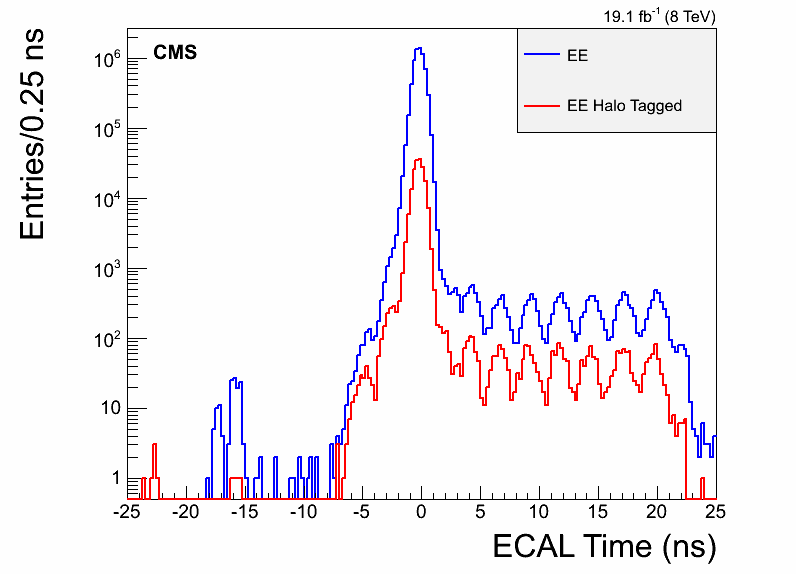
\includegraphics[height=0.45\textwidth, width=0.7\textwidth]{THESISPLOTS/halo_EE_Time.png}
\captionof{figure}{Using $\Delta\phi(\mbox{CSC Seg},\gamma) < 0.05$ to tag photons with $\phi_{\gamma} = 0, \pm \pi$ in the endcaps. A good portion of endcap photon candidates are tagged.}
\label{fig:HALOENDCAP}
\end{center} 
\end{minipage}

\subsubsection{Cosmic Photons} 
Cosmic muons produced in cosmic rays, like beam halo muons, with sufficient energy will radiate~(bremsstrahlung) photons in ECAL. We refer to these photons as \textit{Cosmic Photons}. Unlike halo muons, cosmic muons can arrive at ECAL from any direction at any time. We expect cosmic photons in the barrel produced from cosmic muons, to have hits in the Drift Tubes~(DT) segments found in the muon barrel behind the calorimeters. Using DT segments and  photon supercluster $\eta-\phi$ position in ECAL, we can match cosmic muon hits in DT segments to ECAL photon superclusters within a narrow window in $\Delta\eta$ and $\Delta\phi$. The DT position used in the calculation of $\Delta\eta$ and $\Delta\phi$ is a projection of the muon trajectory using the direction of the DT segment to the outer surface of ECAL because of the large space between the muon barrel and the ECAL. The two dimensional distribution for $\Delta\eta(\mbox{DT Seg},\gamma)$ and $\Delta\phi(\mbox{DT Seg},\gamma)$ of this matching, for events with out-of-time photons; $t_{\gamma} > 2$~ns and $t_{\gamma} < -3$~ns, is shown in the right plot of Figure \ref{fig:COSMIC}. We compared to $\Delta\eta(\mbox{DT Seg},\gamma)$ and $\Delta\phi(\mbox{DT Seg},\gamma)$ distribution for in-time~($|t_{\gamma}| < 1$~ns), shown in the left plot, still in the same figure, we observed that most out-of-time photons have a small $\Delta\eta$ and $\Delta\phi$. Comparing the $\Delta\eta$  and $\Delta\phi$ 2-dimensional distributions of these out-of-time photons to photons from a pure cosmic muons sample~(data taken when no proton-proton collisions is happening), shown in Figure \ref{fig:TRUECOSMIC}, we found a similar small $\Delta\eta$ and $\Delta\phi$ occupancy for the true cosmic muons sample. We conclude that small $\Delta\eta(\mbox{DT Seg},\gamma)$  and $\Delta\phi(\mbox{DT Seg},\gamma)$ can be used to tag and reject events with cosmic photons.

%\paragraph*{}\mbox{}\\
\begin{minipage}{0.90\linewidth} 
\begin{center}
\mbox{
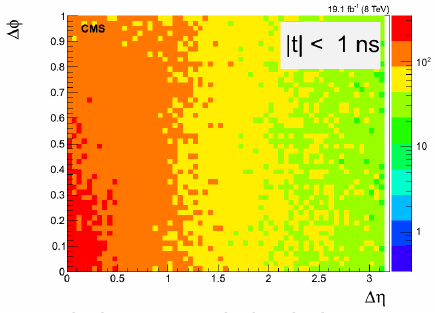
\includegraphics[height=0.45\textwidth, width=0.5\textwidth]{THESISPLOTS/Cosmic_In-time-Photons_Data.png}
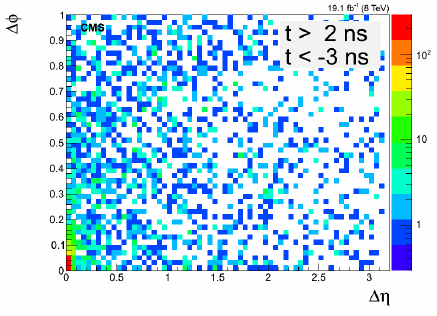
\includegraphics[height=0.45\textwidth, width=0.5\textwidth]{THESISPLOTS/Cosmic_Out-Of-time-Photons_Data.png} 
}
\captionof{figure}{Scatter plot showing $\Delta\eta(\mbox{DT Seg},\gamma)$ against $\Delta\phi(\mbox{DT Seg},\gamma)$ for out-of-time~($ t_{\gamma} > 2$~ns and $t_{\gamma} < -3$~ns) photons~(right) compared to in-time($|t_{\gamma}| < 1$~ns) photons~(left). Cosmic photon candidates have small $\Delta\eta$ and $\Delta\phi$.}
\label{fig:COSMIC}
\end{center}
\end{minipage}

%\paragraph*{}\mbox{}\\
\begin{minipage}{0.90\linewidth} 
\begin{center}
\mbox{
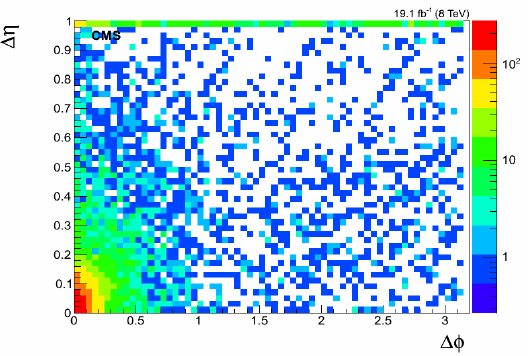
\includegraphics[height=0.45\textwidth, width=0.6\textwidth]{THESISPLOTS/Cosmic_Ray_Photons_Cosmic_dataset.png} }
\captionof{figure}{Scatter plot of $\Delta\eta(\mbox{DT Seg},\gamma)$ against $\Delta\phi(\mbox{DT Seg},\gamma)$ for photons from pure cosmic muon data. Small $\Delta\eta$ and $\Delta\phi$ are cosmic photons.}
\label{fig:TRUECOSMIC}
\end{center}
\end{minipage}

\subsubsection{Anomalous Photons: Spikes}
Neutrons and charge hadrons can at times deposit their energy directly to the APDs instead of going through the crystal scintillation process. Such signals read from the APDs are \textit{anomalous}  and referred to as \textit{spikes}. Spikes produced from $pp$ collisions and satisfying photon selection requirement can easily be identified as photons. A spike supercluster consists of very few crystals; most often one or two crystals. Spikes can also overlapped with real photons and found embedded in a real photon supercluster or buried inside of jets. Such embedded spikes are challenging to identify. By looking at the signal pulse height, the pulse shape for a spike signal appear different from a signal form an electromagnetic particle. Because of this difference in pulse shape profile, the reconstructed ECAL time for spikes usually have large calculated $\chi^{2}$ values.
\newline
The arrival time of spikes is much earlier~(negative), usually about $t \approx -12.0$~ns than for photons produced in nominal $pp$ collisions depositing their energy in the APD through crystal scintillation. This is because of the absence of the scintilation process which takes on average 10~ns. The few crystals containing the spike cluster energy deposits make it possible for spikes to be identified using a energy topological selection quantity, $1-\frac{E_{4}}{E_{1}}$, also know as \textit{swiss-cross} variable.  By looking at a distribution shown in right plot of Figure 
\ref{fig:SPIKES}, of the swiss-cross for in-time and for events from a spike sample~(events with photon with time $t = -12$~ns),  we observed that most spikes have about 98\% of their energy deposited in a single crystal.
\newline
Using the number of crystals in a photon supercluster and comparing the number of crystals in in-time photons to halo photons and spike candidate photons~(photons with $1-\frac{E_{4}}{E_{1}}> 0.98$) shown in the left plot of Figure \ref{fig:SPIKES}, we observed that most spikes including spikes embedded in electromagnetic candidates have less than $7$ crystals in their supercluster. A combination of the swiss-cross, number of crystals in supercluster, calculated $\chi^{2}$ from ECAL time, $S_{Major}$ and $ S_{Minor}$~(both $S_{Major}$ and $ S_{Minor}$ describe the shape of the electromagnetic shower) is useful for identifying and rejecting events with spikes.

\vspace{5mm}
\begin{minipage}{0.90\linewidth} 
\begin{center}
\captionsetup{type=figure}
\mbox{
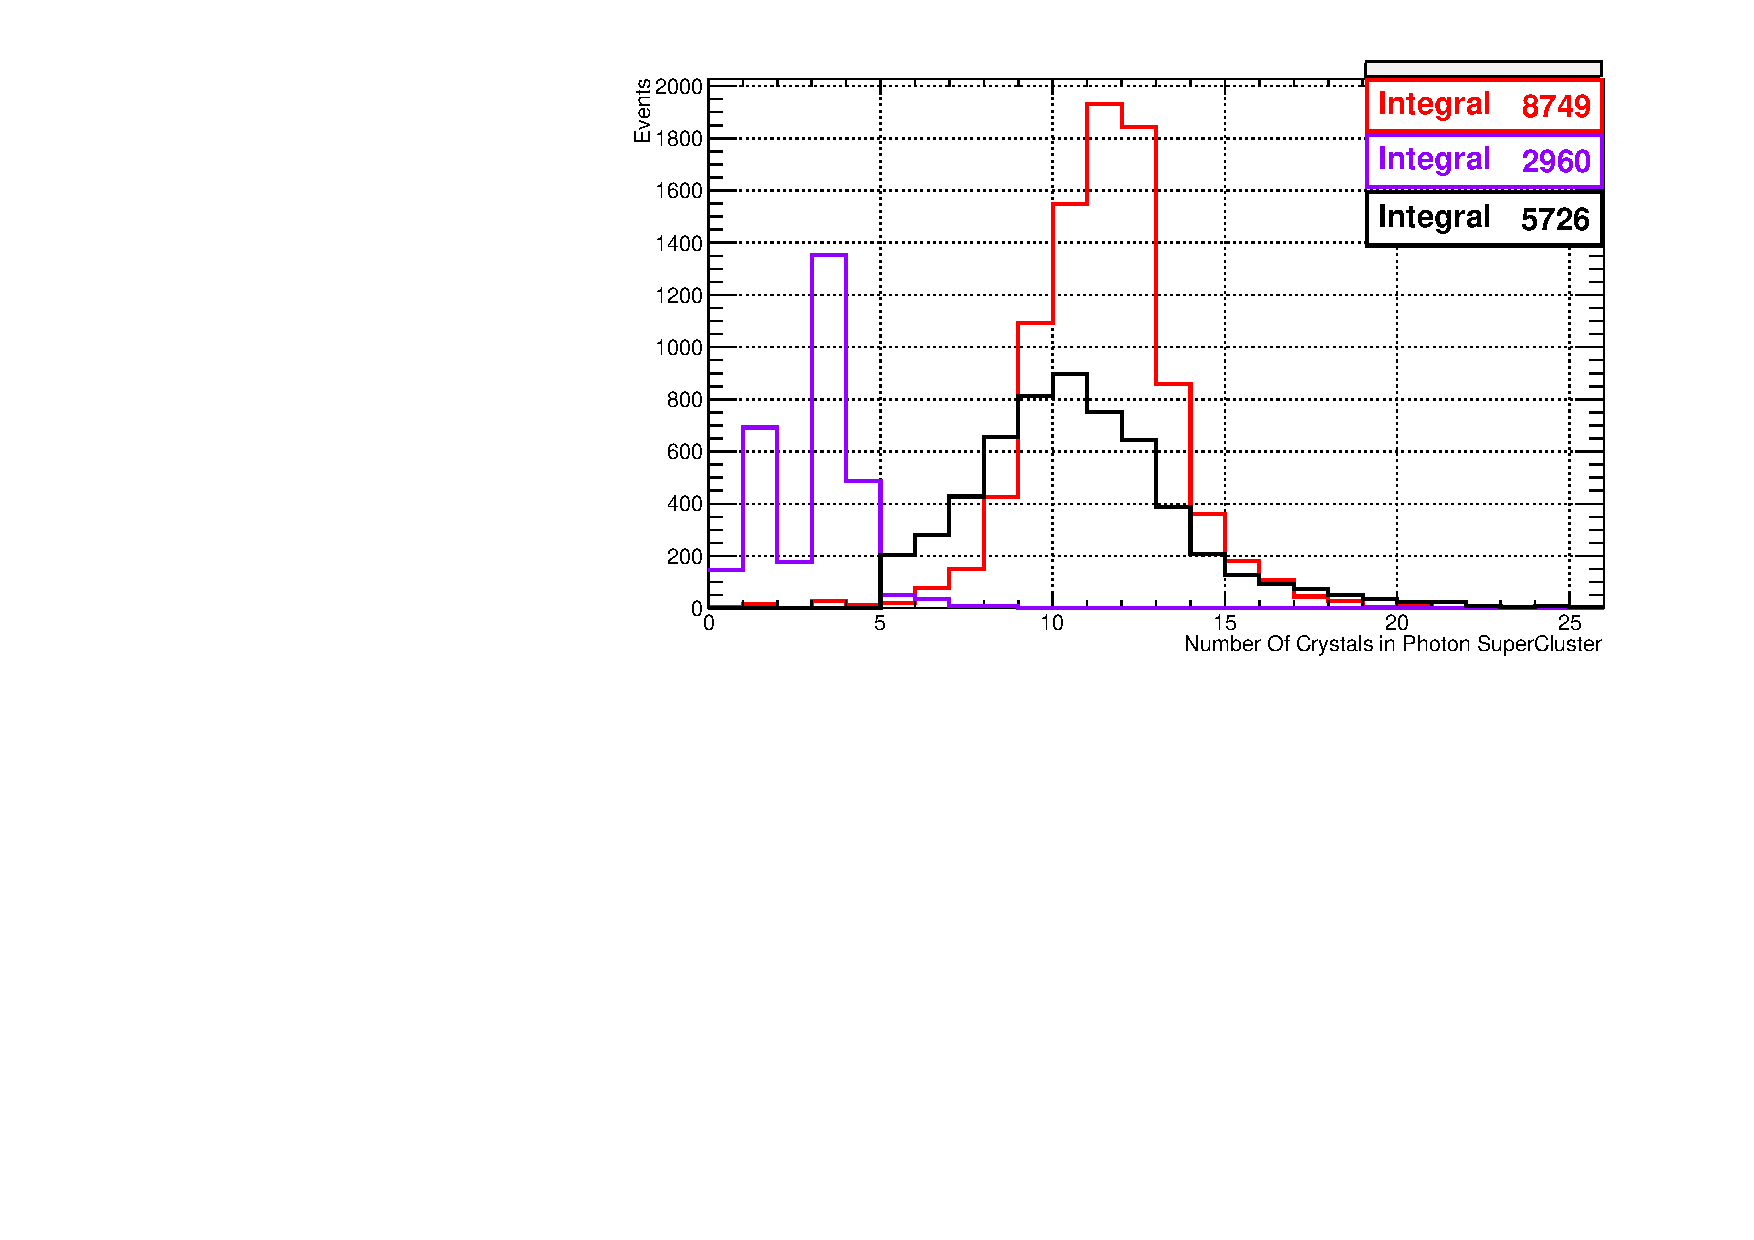
\includegraphics[height=0.50\textwidth, width=0.5\textwidth]{THESISPLOTS/Number-Of-Crystals-In-Photon-SC.pdf}
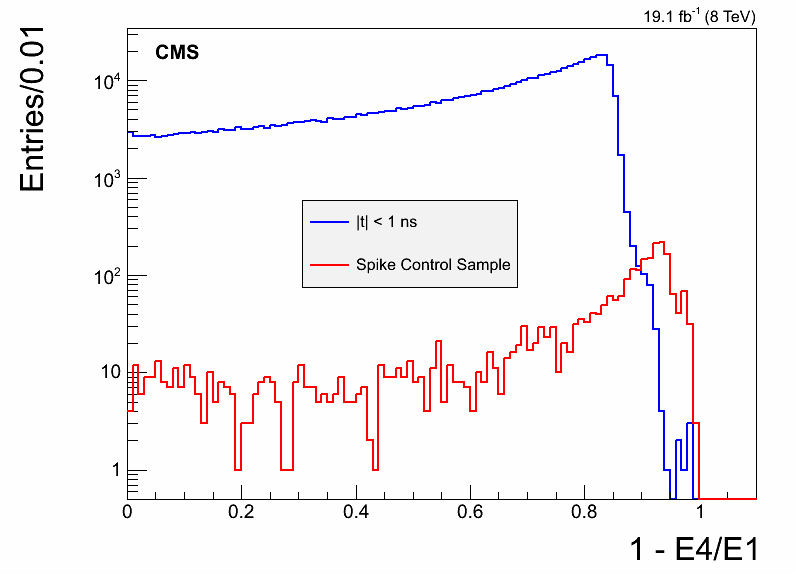
\includegraphics[height=0.50\textwidth, width=0.5\textwidth]{THESISPLOTS/swissX.png} }
\captionof{figure}{\textit{Number of crystals} in photon supercluster plot~(Left) for in-time photon candidates~(black), spike photon candidates~(magenta) and halo photon candidates~(red). The spike photon candidates are selected with an energy swiss-cross variable~($1- E_{4}/E_{1}$)~(right) shown comparing in-time photons~($|t_{\gamma}| < 1.0 $) to spike candidate sample selected with $ S_{Minor}$ and $S_{Major}$ variables.}
\label{fig:SPIKES}
\end{center}
\end{minipage}

\subsection{Event Vetoing, Performance and Fake Rates}
Using the quantities studied for tagging events with halo, cosmic and spike photons, we tag and veto non-collision background  events as follows: 
\begin{itemize}
\item An event with a halo photon is tagged and vetoed if a CSC segment for $|\eta| > 1.6$ is found within 0.05 radian of the azimuthal angle with the photon supercluster, \ie a photon found within $\Delta\phi(\mbox{CSC Seg},\gamma) < 0.05$ is vetoed. We found that we are able to veto events with a  halo photon with 91\% efficiency and 3\% mis-tag rate using this photon selection requirement.
\item An event with cosmic photon is tagged and vetoed with $75.5$\% efficiency and $1.4$\% mis-tag rate if the photon can be matched to a DT segment within $\Delta\eta(\mbox{DT Seg},\gamma) < 0.1$ and $\Delta\phi(\mbox{DT Seg},\gamma) < 0.1$.
\item An event with spike is vetoed if the photon has ECAL time $\chi^{2} > 4$, $\mbox{Number of crystals} < 7$, $ 1-E_{4}/E_{1} > 0.98$,$S_{Major} < 0.6$ and $S_{Minor} < 0.17$ with only $0.4$\% mis-tag rate.
\end{itemize}
Presented in Table \ref{tab:EVTC}, is a summary for the mis-tag rates of the different non-collision background sources. 

%%\paragraph*{}\mbox{}\\
\begin{minipage}{0.90\linewidth} 
\begin{center}
\begin{tabular}{|c| c|}
%\mbox{Fake Rate }
\hline
\bfseries{Background Source} & \bfseries {Fake Rate}(\%)\\
\hline\hline
\textit{Halo Photons} & ~$\approx 3$ \\
\textit{Cosmic Photons} & ~$\approx 1.4$ \\
\textit{Spikes} & $\approx 0.4$ \\
\hline
\end{tabular}
\captionof{table}{Fake rates for different non-collision vetoing.}
\label{tab:EVTC} 
\end{center}
\end{minipage}

\vspace{5mm}
The result of the event tagging is shown in Figure \ref{fig:RESIDUAL}. We observe that the majority of non-collision background events are events with a halo photon. Very few late arrival time photons are produced from spikes. The is also some significant contribution from cosmic photons. The most interesting observation is the residual out-of-time background~(in red) which could not be tagged. 

\paragraph*{}\mbox{}\\
\begin{minipage}{0.90\linewidth} 
\begin{center}
  \captionsetup{type=figure}
   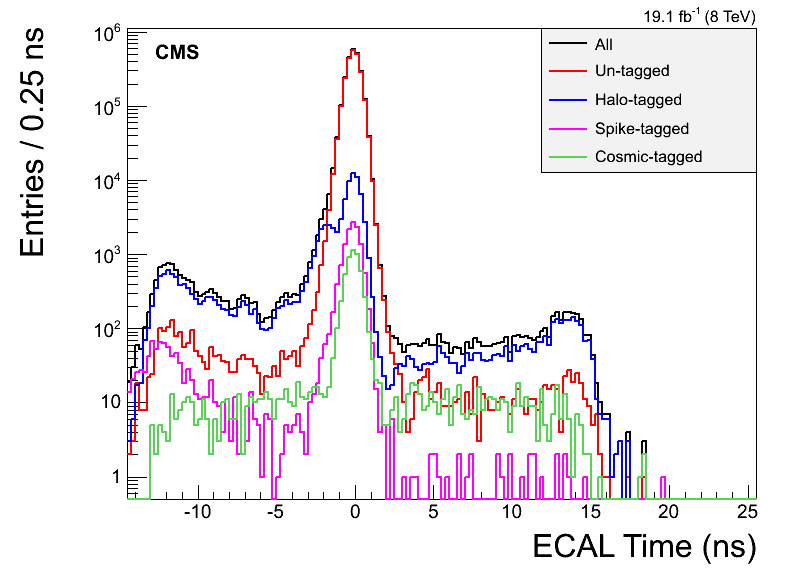
\includegraphics[height=0.7\textwidth, width=0.8\textwidth]{TimeForAll}
%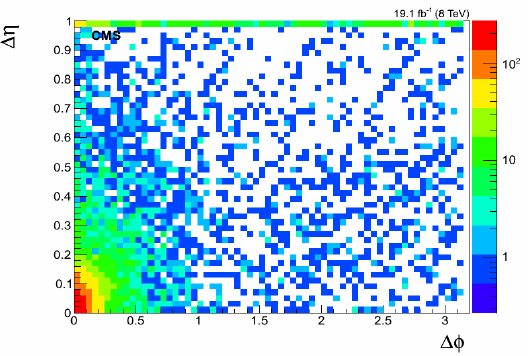
\includegraphics[height=6cm, width=0.5\textwidth]{THESISPLOTS/Cosmic_Ray_Photons_Cosmic_dataset.png} 
   \captionof{figure}{ECAL photon time for a data sample of 0 and 1-jet events showing our tagging performance for non-collision background events.}
   \label{fig:RESIDUAL}
\end{center}
\end{minipage}

\vspace{5mm}
These residual untagged events comprise of some non-collision events, since the tagging and vetoing are not 100\% efficient, events with QCD photons from ghost/satellite collisions and events with $\PW\rightarrow \Pe\Pagne$ decay with the fake photon passing the photon selection requirement. In order to quantify our estimates of these different sources contributing to the untagged background events, we use control samples defined with ${\ETslash}^{\gamma}\hspace{0.15cm}$ and \ETslash\hspace{0.25cm}. %, recalling that $\vec{{\ETslash}^{\gamma}\hspace{0.15cm}} = \vec{\ETslash\hspace{0.15cm}} + \vec{\pt^{\gamma}}$ adjusting for out-of-time energy deposits not included in the standard missing transverse energy calculations. 
\newline
We expect signal events, because of the undetected gravitino from the neutralino decay, to have large ${\ETslash}^{\gamma}\hspace{0.15cm}$ and \ETslash\hspace{0.15cm}, by large, we mean above 60\GeV, and events with $\PW\rightarrow \Pe\Pagne$ decay to equally have large ${\ETslash}^{\gamma}\hspace{0.15cm}$ and \ETslash\hspace{0.15cm} because of the undetected neutrino. The non-collision~(cosmic, halo, spike) and collision~(ghost/sattelite or QCD) background events can be categorized into high-\pt and low-\pt events.
For high-\pt non-collision events, we expect these events to have large \ETslash\hspace{0.15cm}, due to the exclusion of the energy deposits from the out-of-time photons in the missing transverse energy reconstruction, and small ${\ETslash}^{\gamma}\hspace{0.15cm}$ when the large transverse energy contribution from the energy deposits of the out-of-time photons is re-introduced, while for low-\pt non-collision events, we expect these events to have both ${\ETslash}^{\gamma}\hspace{0.15cm}$ and \ETslash\hspace{0.15cm} small, since the out-of-time photon transverse energy, which was excluded, was in the first place small. For high-\pt out-of-time collision events which usually have small missing transverse energy, we expect their \ETslash\hspace{0.25cm} to be small and after re-introducing the energy deposits from out-of-time high-\pt photons, we expect their ${\ETslash}^{\gamma}\hspace{0.15cm}$ to be large, while, using the same argument made for low-\pt non-collision events, we expect low-\pt collision events to have both small ${\ETslash}^{\gamma}\hspace{0.15cm}$ and \ETslash\hspace{0.15cm}.
A summary of our expectations for ${\ETslash}^{\gamma}\hspace{0.15cm}$ and \ETslash\hspace{0.15cm} for the different expected background events sources with possible contribution to the residual untagged events with out-of-time photon is presented in Table \ref{tab:METSAMPLE}.

\vspace{5mm}
\begin{minipage}{0.90\linewidth} 
  \begin{center}
   \begin{tabular}{c| c|c}
   \toprule
   \hline
     \bfseries{Event Sample} & $\mathbf{\ETslash\hspace{0.15cm}}$ &          $\mathbf{{\ETslash}^{\gamma}\hspace{0.15cm}}$\\
    \hline
    \toprule
   
     Signal Events & Large & Large \\
     $\PW\rightarrow \Pe\Pagne$ Events & Large & Large \\
     High-\pt Non-Collision(Mostly Beam Halo) Events & Large & Small \\
     Low-\pt Non-Collision Events & Small & Small \\
     High-\pt Collision(QCD/Ghost) Events & Small & Large \\
     Low-\pt Collision Events & Small & Small \\
     \hline
   \bottomrule     
   \end{tabular}
   \captionof{table}{Summary of missing transverse expectation for events with out-of-time photons.}
   %\caption{\textsf{ABCD} Control Regions~(CRs) for estimating non-collision background.}
   \label{tab:METSAMPLE} 
 \end{center}
\end{minipage}

\vspace{5mm}
%Therefore, to minimizing contributions from events anomalous photon time, we restrict our photon arrival time for signal events to within $3.0 < t_{\gamma} < 13.0$~ns, while also requiring that the signal event missing transverse energy be greater than 60\GeV, \ie ${\ETslash}^{\gamma}\hspace{0.15cm} > 60$\GeV, $\ETslash\hspace{0.15cm} > 60$\GeV. This reduces the contribution from ghost/satellite background contributing to the untagged out-of-time photons while at the same time enhances our signal event sample.
\clearpage
Using control samples defined using \ETslash\hspace{0.15cm} and ${\ETslash}^{\gamma}\hspace{0.15cm}$ for events with in-time~($|t_{\gamma}| < 2.0$~ns) photons, 
events with photon time, $t_{\gamma} > 3.0$~ns and $t_{\gamma} < -3.0$~ns, where each control sample is defined purposely to enhance the contribution of either collision or non-collision background events to that control sample while simultaneously suppressing contributions from the other, we perform a background estimation in the signal control sample~($t_{\gamma} > 3.0$~ns, ${\ETslash}^{\gamma}\hspace{0.15cm} > 60$\GeV and $\ETslash\hspace{0.15cm} > 60$\GeV) using the so-called \textsf{ABCD} background estimation method.
We verify that the background estimation method is performing as expected using a data sample of zero and one jet events.
% with out-of-time photons, $t_{\gamma} > 3.0$~ns and  ${\ETslash}^{\gamma}\hspace{0.15cm} > 60$\GeV, $\ETslash\hspace{0.15cm} > 60$\GeV  is supposed to be the same if the method is valid. One of our assumption for using the ABCD method is that the background contributions from QCD events and multijets events is negligible. We also study the consequences of this assumption on the number of background estimated events with a separate control sample of mostly out-of-time photon candidates used in reconstructing the true \PZ mass and measure the its candidate electron's arrival time at ECAL since for these events we expect most of the electrons from the $\PZ \rightarrow \EE$ decay to be in-time. Thus, the observed number of out-of-time electron candidates gives us an estimate of the contributions of collision events in our signal sample.

%%\begin{figure}[htbp]
%%  \begin{center}
%%    \captionsetup{type=figure}
%%     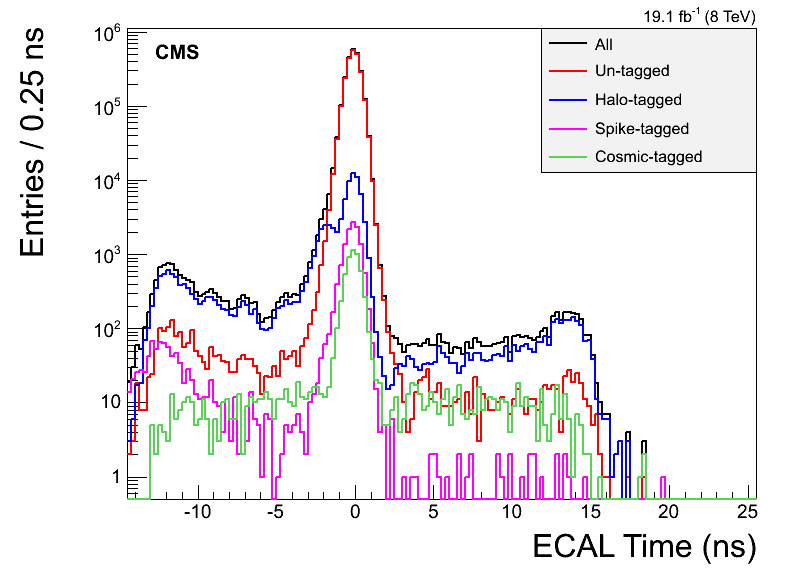
\includegraphics[height=0.7\textwidth, width=0.8\textwidth]{TimeForAll}
%%    \caption{Residual Background(red) after tagging the different non-collision background sources using the selection variables described in text.}
%%    \label{fig:RESIDUAL}
%%   \end{center}
%%\end{figure}
%%\begin{table}[h!]
%% \begin{center}
%%   \begin{tabular}{| l c r |}
%%   \hline
%%   1 & 2 & 3 \\
%%   4 & 5 & 6 \\
%%   7 & 8 & 9 \\
%%   \hline
%%   \end{tabular}
%% \end{center}
%%\caption{A simple table}
%%\end{table}
%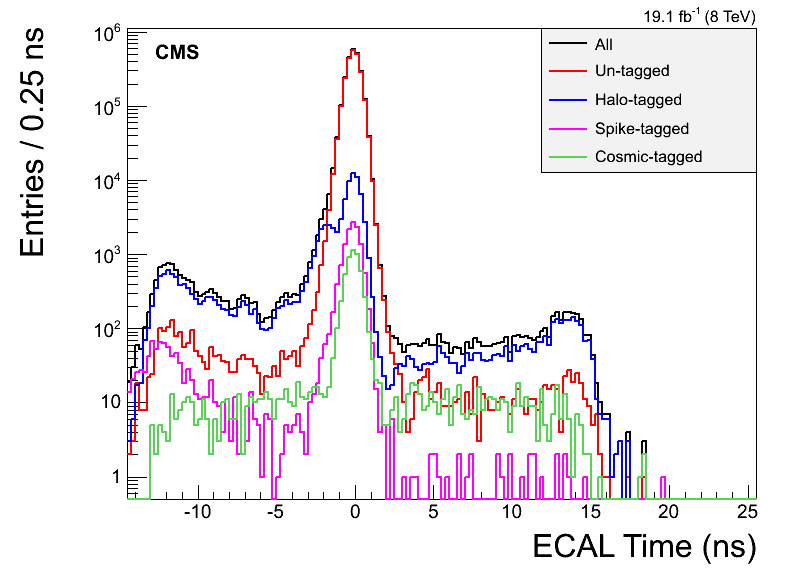
\includegraphics[height=0.7\textwidth, width=0.8\textwidth]{TimeForAll}
%\end{figure}
\subsection{Background Estimation with ABDC Method}
Since we expect most of our background events to come from non-collision events, we estimate the number of events we expect from non-collision events in the signal control sample using the \textsf{ABCD} technique. We also estimate the possible contamination, we expect from collision events, to the control samples used in the \textsf{ABCD} method.
\begin{enumerate}
\item \textbf{Non-Collision Background Estimation}:\newline
To estimate the number of background events from non-collision, we define Control Samples~(CS), labeled as \textsf{ABCD}, in photon ECAL time and ${\ETslash}^{\gamma}\hspace{0.15cm}$ for selected events with $\ETslash\hspace{0.15cm} > 60$\GeV. Events with $\ETslash\hspace{0.15cm} > 60$\GeV define a CS  where the contribution from collision~(QCD) background events is suppressed, since most collision background events have small \ETslash\hspace{0.15cm}, as we saw in Table \ref{tab:METSAMPLE}. The control samples; \textsf{A} and \textsf{B}, shown in Table \ref{tab:NON-COLLISION}, are events with, respectively, ${\ETslash}^{\gamma}\hspace{0.15cm} < 60$\GeV and ${\ETslash}^{\gamma}\hspace{0.15cm} > 60$\GeV  and photon ECAL time, $-10.0 < t_{\gamma} < -3.0$~ns, and CS \textsf{C} have events with ${\ETslash}^{\gamma}\hspace{0.15cm} < 60$\GeV  and photon ECAL time, $3.0 < t_{\gamma} < 13.0$~ns.

\vspace{5mm}
\begin{minipage}{0.90\linewidth} 
  \begin{center}
   \begin{tabular}{|c| c| c|}
   \hline
     \bfseries{Non-Collision} & $\mathbf{{\ETslash}^{\gamma}\hspace{0.15cm}} < 60$\GeV & $\mathbf{{\ETslash}^{\gamma}\hspace{0.15cm}} > 60$\GeV \\     
      \hline \hline
        $3.0 < t_{\gamma} < 13.0$~ns. &  \textsf{$C$} &  \textsf{$D$} \\
      \hline
        $ -10.0 < t_{\gamma} < -3.0$~ns & \textsf{$A$} &  \textsf{$B$} \\
    \hline 
   \end{tabular}
   \captionof{table}{\textsf{ABCD} Control Samples~(CSs) definitions used for estimating non-collision background events in the signal CS \textsf{D}. Events must satisfy the $\ETslash\hspace{0.15cm} > 60$\GeV selection requirement.}
   %\caption{\textsf{ABCD} Control Regions~(CRs) for estimating non-collision background.}
   \label{tab:NON-COLLISION} 
  \end{center}
 \end{minipage}
%%\end{table}
%\begin{itemize}
%\item \textbf{A}: Events with ${\ETslash}$~~$ < 60$~GeV and $ -10.0 < t_{\gamma} < -3.0$~ns.
%\item \textbf{C}: Events with ${\ETslash}$~~$ < 60$~GeV and $3.0 < t_{\gamma} < 13.0$~ns.
%\item \textbf{B}: events with ${\ETslash}$~~$ > 60$~GeV and $-10.0 < t_{\gamma} < -3.0$~ns.
%\item \textbf{D}: events with ${\ETslash}$~~$ > 60$~GeV and $3.0 < t_{\gamma} <  13.0$~ns.
%\end{itemize}

\vspace{5mm}
 Using these control samples for the \textsf{ABCD}  method, and with the assumption that $\frac{N_{D}}{N_{C}} = \frac{N_{B}}{N_{A}}$, the number of non-collision background events with out-of-time photons expected in the signal  CS \textsf{D} is given as
\begin{equation}
N^{non-col}_{D} = \left(\frac{N_{B}}{N_{A}} \right)\cdot N_{C},
\end{equation}
where $N_{B}$, $N_{A}$  and $N_{C}$ are the number of events observed in \textsf{B}, \textsf{A} and \textsf{C} control samples in that order and $N^{non-col}_{D}$ is the number of non-collision background events we expect in the signal CS \textsf{D}.

\item\textbf{Collision Background Estimation}:\newline
We estimate the number of collision background events contaminating CSs defined in Table \ref{tab:NON-COLLISION}, by once again using the \textsf{ABCD} technique with the Control Samples~(CSs) used defined in photon ECAL time and \ETslash\hspace{0.15cm} for selected events with ${\ETslash}^{\gamma}\hspace{0.15cm} > 60$\GeV. We are interested in the contamination from collision background events to CS \textsf{B} and \textsf{D} of Table \ref{tab:NON-COLLISION}, since these are the CSs where we expect events with large missing transverse energy~(see Table \ref{tab:METSAMPLE}).
Most collisions events have photons with in-time~($|t_{\gamma}| < 2$~ns), therefore, we use CSs defined with in-time photons to estimate the number of possible collision events with out-of-time photons contributing to CSs \textsf{B} and \textsf{D}. The CSs used for the new \textsf{ABCD} method to perform the collision background estimation are labeled as \textsf{$A^{\prime}$ $B^{\prime}$ $C^{\prime}$  $D^{\prime}$} and defined as shown in Table \ref{tab:COLLISION}. 

\vspace{5mm}
\begin{minipage}{0.90\linewidth} 
\begin{center}
\begin{tabular}{|c| c| c|}
 \hline
\bfseries{Collision}       & $\mathbf{\ETslash\hspace{0.15cm} } < 60$\GeV &  $\mathbf{\ETslash\hspace{0.15cm}} > 60$\GeV \\      
\hline \hline
$3.0 < t_{\gamma} < 13.0$~ns. &  \textsf{$C^{\prime}$} &  \textsf{$D^{\prime}$} \\
\hline
$ -2.0 < t_{\gamma} < 2.0$~ns & \textsf{$I^{\prime}$} &  \textsf{$I$} \\
\hline 
$ -10.0 < t_{\gamma} < -3.0$~ns & \textsf{$A^{\prime}$} &  \textsf{$B^{\prime}$} \\
\hline
\end{tabular}
\captionof{table}{\textsf{$A^{\prime}$ $B^{\prime}$ $C^{\prime}$ $D^{\prime}$} and \textsf{$I$ $I^{\prime}$} Control Samples~(CSs) used for estimating collision background events contamination to CSs \textsf{B} and \textsf{D}. Events here must satisfy ${\ETslash}^{\gamma}\hspace{0.15cm} > 60$\GeV selection requirements. }
\label{tab:COLLISION} 
\end{center}
\end{minipage}

\vspace{5mm}
The number of collisions events contributing to the CS \textsf{B}, $N_{B}^{col}$, is estimated as 
\begin{equation}{\label{eq:COLB}}
\displaystyle{N_{B}^{col} = N_{B^{\prime}}  = \left( \frac{I}{I^{\prime}} \right)\cdot N_{A^{\prime}}}, 
\end{equation}
while the number of events contributing to the CS \textsf{D}, $N_{D}^{col}$, is estimated as
\begin{equation}{\label{eq:COLD}}
\displaystyle{N_{D}^{col} = N_{D^{\prime}}  = \left( \frac{I}{I^{\prime}} \right)\cdot N_{C^{\prime}}},
\end{equation}
where the general assumption is that $\frac{N_{B^{\prime}}}{N_{A^{\prime}}}  = \frac{N_{I}}{N_{I^{\prime}}}$ and  $\frac{N_{D^{\prime}}}{N_{C^{\prime}}}  = \frac{N_{I}}{N_{I^{\prime}}}$, with each $N_{i}$ being the number of events in each CS $i=$ \textsf{$A^{\prime}$, $B^{\prime}$, $C^{\prime}$, $D^{\prime}$, $I$, $I^{\prime}$}.
%\begin{itemize}
%\item $\mathbf{A^{\prime}}$: Events with ${\ETslash}^{\gamma} < 60$~GeV and $-10.0 < t_{\gamma} < -3.0$~ns.
%\item $\mathbf{B^{\prime}}$: Events with ${\ETslash}^{\gamma} > 60$~GeV and $-10.0 < t_{\gamma} < -3.0$~ns.
%\item $\mathbf{I^{\prime}}$: Events with ${\ETslash}^{\gamma} < 60$~GeV and $|t_{\gamma}| < 2.0$~ns.
%\item $\mathbf{I}$: Events with ${\ETslash}^{\gamma} > 60$~GeV and $|t_{\gamma}| < 2.0$~ns.
%\end{itemize}
%we also define a in time CR as:
%\begin{itemize}
%\item $\mathbf{C^{\prime}}$: Events with ${\ETslash}^{\gamma} < 60$~GeV and $ 3.0 < t_{\gamma} <  13.0$~ns.
% \item $\mathbf{D^{\prime}}$: Events with ${\ETslash}^{\gamma} > 60$~GeV and $3.0 < t_{\gamma} <  13.0$~ns.
% \item $\mathbf{I^{\prime}}$: Events with ${\ETslash}^{\gamma} < 60$~GeV and $|t_{\gamma}| < 2.0$~ns.
%\item $\mathbf{I}$: Events with ${\ETslash}^{\gamma} > 60$~GeV and $|t_{\gamma}| < 2.0$~ns.
%\end{itemize}
\item \textbf{Combined Background Estimation}: \newline
Now that we have estimates for both collision and non-collision event contributions, we can estimate the total number of background events expected in the signal CS \textsf{D}~(Events with $\ETslash\hspace{0.15cm} > 60$\GeV, ${\ETslash}^{\gamma}\hspace{0.15cm} > 60$\GeV and $3.0 < t_{\gamma} < 13.0$~ns), as
\begin{equation}{\label{eq:FBKG}}
N_{D}^{Total} = \left(\frac{N_{B} - N_{B}^{col} }{N_{A}} \right)\cdot N_{C} + N_{D}^{col} = N_{D}^{non-col} + N_{D}^{col}
\end{equation}
where $N_{D}^{Total} = N_{D}^{non-col} + N_{D}^{col}$ is the total background events estimated in our signal CS \textsf{D} coming from non-collision and collision background events. 
\end{enumerate}
%\begin{center}
%\centering
%\mbox{
%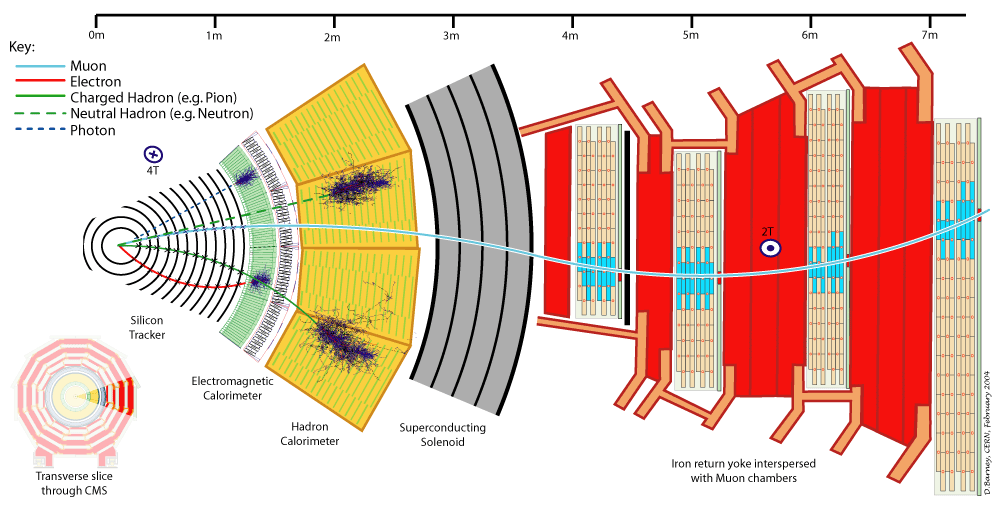
\includegraphics[scale=0.2]{THESISPLOTS/CMS_Slice.png}
%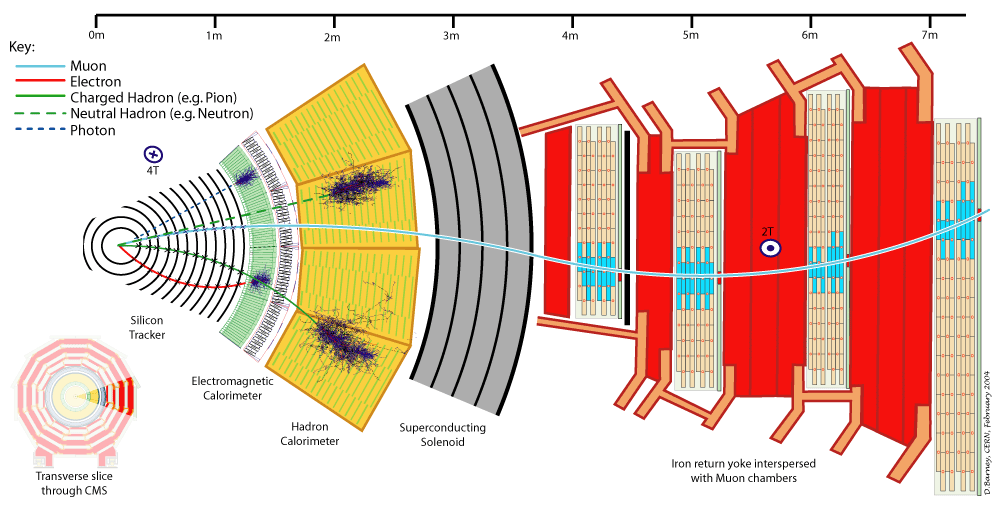
\includegraphics[scale=0.2]{THESISPLOTS/CMS_Slice.png}
%\captionof{figure}{Diagrams showing background estimation technique.}
%\label{fig:BKGESTI}
%\end{center}
\paragraph*{Background Estimation Technique Validation}\mbox{}\\
We performed a validity test of our background estimation method using a data sample of $0$ and $1$-jet events, where we do not expect any signal events.
A statistical agreement in the number of expected background events obtained using our background estimation method and the number of events observed in our signal CS \textsf{D}, will indicate provide a positive affirmation that the method. The accepted $0$ and $1$-jet events used must pass the same event selection requirements as potential signal events described in Tables \ref{tab:PhotonSel} and \ref{tab:JetSel}. The event yields in each control sample including the tagging of beam-halo, cosmic and spike events is shown in Table \ref{tab:EVTYIELD}.

\vspace{5mm}
\begin{minipage}{0.90\linewidth} 
\begin{center}
\begin{tabular}{c| c| c| c| c }
\toprule
 \hline
\bfseries{Control Sample} & Yield & Beam Halo & Cosmic & Spike \\
\hline
\toprule
\textsf{A} & 852 & 5075 & 237 & 65\\
\textsf{B} & 39 & 300&  17 &  1\\
\textsc{C} & 359 & 1508 & 368 & 9  \\
\textsf{D} & 10 & 22 & 30 & 0 \\
\hline\hline
\textsf{$A^{\prime}$}& 8 &  1& 1 & 0\\ 
\textsf{$C^{\prime}$}& 2 & 0 & 0 & 0\\  
\textsf{$I$} & 35464 & -& - & -\\    
\textsf{$I^{\prime}$}&  1446522 & - & - & \\       
\textsf{$B^{\prime}$}& - &-  & - & -\\    
\textsf{$D^{\prime}$}& - & - & - & -\\      
\hline
\bottomrule
\end{tabular}
\captionof{table}{Event yields used in validity test for the \textsf{ABCD} background estimation method using $0$ and $1$-jet events sample. Beam halo/cosmic/spikes yields are obtained from tagged events. Events must pass photon, jet and \MET selection requirements.}
\label{tab:EVTYIELD} 
\end{center}
\end{minipage}

\vspace{5mm}
Using the event yields in Table \ref{tab:EVTYIELD} for each CS, and Equations \ref{eq:COLB}, \ref{eq:COLD} and \ref{eq:FBKG}, we obtain the following estimates for the expected number of events in signal CS \textsf{D} as
\begin{align*} 
 N_{B}^{col} &= \frac{35464}{1446522} \times 8 = 0.20^{+0.08}_{-0.06} \\
 N_{D}^{col} &= \frac{35464}{1446522} \times 2 = 0.05^{+0.05}_{-0.02} \\
 N_{D}^{Total} &= \left( \frac{39 - 0.20}{852}\times 359\right) +  0.05 = 16.40^{+3.04}_{-2.63}.
\end{align*}
The uncertainty are statistical uncertainties based on the event statistics in each CS. Our expected number of background events in signal CS \textsf{D} is $16.40^{+3.04}_{-2.63}$  which is, within the statistical uncertainties, agreeable with the 10 events we observed satisfying all our event selection requirements and belonging to the CS \textsf{D}. 
This give us confidence that our method is working and should be used in our background estimation method for potential signal events from data sample.
% We observed $10$ events while from using Equation \ref{eq:FBKG}, we expected $16.78^{+2.95}_{-3.45}$. We argue that within our statistical uncertainties, there is quite an agreement between our expectation and observed events. The complete result from our closure test is shown in Table \ref{tab:EVTC}. This gives us confidence that our  background estimation method is robust and reliable. We apply the same \textsf{ABCD} to estimate the background contribution in our signal sample. Our signal sample consist of events with at least $2$-jets, at least a single photon and ${\ETslash}^{\gamma}\hspace{0.15cm} > 60$\GeV, $\ETslash\hspace{0.15cm} > 60$\GeV
%\paragraph*{}\mbox{}\\
%\begin{minipage}{\linewidth} 
%\begin{center}
%\begin{tabular}{|c| c| c|}
%\mbox{Fake Rate }
%\hline
%\bfseries{Non-Collision} &  $\mathbf{{\ETslash}^{\gamma}\hspace{0.15cm}} < 60$\GeV & $\mathbf{{\ETslash}^{\gamma}\hspace{0.15cm}} > 60$\GeV \\
%\hline
% $3.0 < t_{\gamma} < 13.0$~ns & \textsf{C}($405$) & ~\textsf{D}($10$) \textcolor{blue}{16.78} \\
% $-10.0 < t_{\gamma} < -3.0$~ns & \textsf{A}($871$) & ~\textsf{B}($36$) \\
%\hline \hline
%\bfseries{Collision} & $\mathbf{\ETslash\hspace{0.15cm}} < 60$\GeV & $\mathbf{\ETslash\hspace{0.15cm}} %> 60$\GeV \\
%\hline 
% $3.0 < t_{\gamma} < 13.0$~ns & \textsf{$D^{\prime}$}($4$) & ~\textsf{D}($10$) \\
% $-2.0 < t_{\gamma} < 2.0$~ns & \textsf{$F^{\prime}$}($1353685$) & ~\textsf{F}($34543$) \\
% $-10.0 < t_{\gamma} < -3.0$~ns & \textsf{$B^{\prime}$}($5$) & ~\textsf{B}($36$) \\
%\hline 
%\end{tabular}
%\captionof{table}{Result from closure test of background estimation technique using 0 and 1-jet events. Numbers in bracket represent our expected background estimate using \textsf{ABCD} method.}
%\label{tab:EVTC} 
%\end{center}
%\end{minipage}
\subsection{Background Estimation Cross Check}
Another method for estimating background events with out-of-time photons from collision, which we did, is using $\PZ \rightarrow \EE$ events. Since we expect most of the events with electron candidates from \PZ decay to be in-time due to the prompt nature of the decay of \PZ bosons, we use events with electron candidates from a \texttt{SingleElectron} and \texttt{DoubleElectron} data samples of 2012, where we expect the contributions from non-collision events to be very small, to do the estimation. These events are selected such that out-of-time energy deposits in ECAL from electron candidates are accepted. The background events with out-of-time energy deposits are mostly events produced from the Drell-Yan process, where electron candidates can be matched randomly to produce a di-electron mass close to the mass of \PZ and poorly reconstructed out-of-time  energy deposits in ECAL. To further reduce any out-of-time contribution from beam halo and cosmic events, which can occur simultaneously with true $pp$ collision events, we require that events with \PZ candidates must satisfy the following event selection requirements: the two electron candidates of the \PZ boson must each have a $\pt > 30$\GeV/c, di-electron mass, $|m_{\EE} - 91| > 61$\GeV/cc, and both electrons must be in the barrel, \ie $|\eta_{e^{-}}| < 1.479$ and $ |\eta_{e^{+}}| < 1.479$.
\newline
From these selected \PZ candidate events, we define a signal event sample where the \PZ candidates have a well defined di-electron mass between $76 < |m_{\EE}| < 100$~$GeV/c^{2}$ and a background or sideband event sample where the di-electron mass is either between $50\GeVcc < m_{\EE} < 76$\GeVcc or $100\GeVcc < m_{\EE} < 130$\GeVcc. 
\newline
The electron ECAL arrival time is taken to be the seed crystal time adjusted to account for the electron time of flight. The seed crystal must satisfy the recommended crystal~(reconstructed hit) cleaning criteria which requires that the seed crystal is not a spike, is not noisy and has been properly time calibrated.
A scatter plot of the arrival ECAL time against $\eta$~(top plots) and  $\phi$~(bottom plots) of the electron candidate of \PZ is shown in Figure \ref{fig:Elec}. A clear difference in the scatter distributions of events is seen comparing events from the \texttt{Single/DoubleElectron} data sample~(plots on the right) which do not have the familiar beam halo features~(the X-shape and increase event population around $\phi = 0,\pm \pi$) to events from \texttt{SinglePhoton} data sample~(plots on the left). 
This confirms our expectation that the candidate \PZ event sample is free from contamination from non-collision events and thus a good sample for estimating out-of-time event contributions from collisions.

\vspace{5mm}
\begin{minipage}{0.90\linewidth} 
\begin{center}
\mbox{
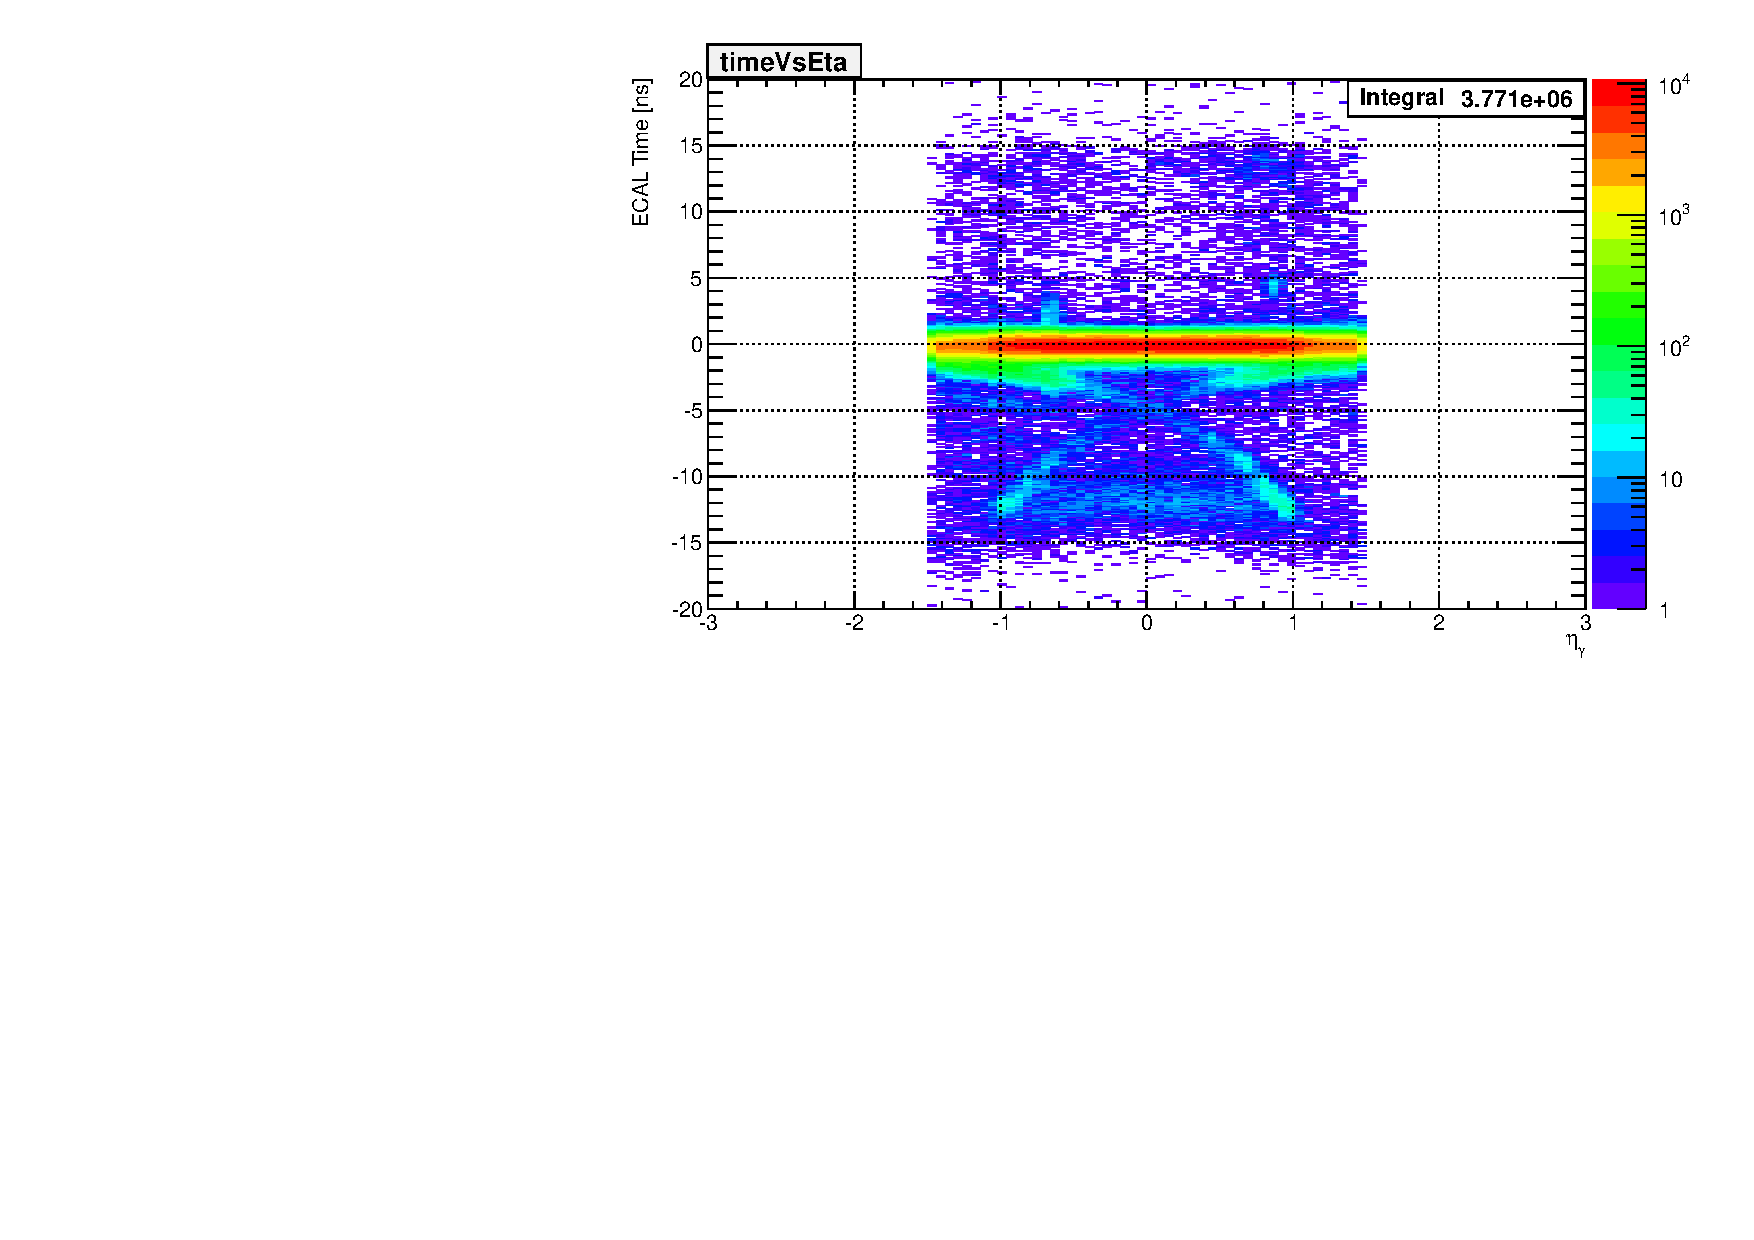
\includegraphics[height=0.340\textwidth, width=0.5\textwidth]{THESISPLOTS/SinglePhotonDataSet-TimeVsEtaEB.pdf}
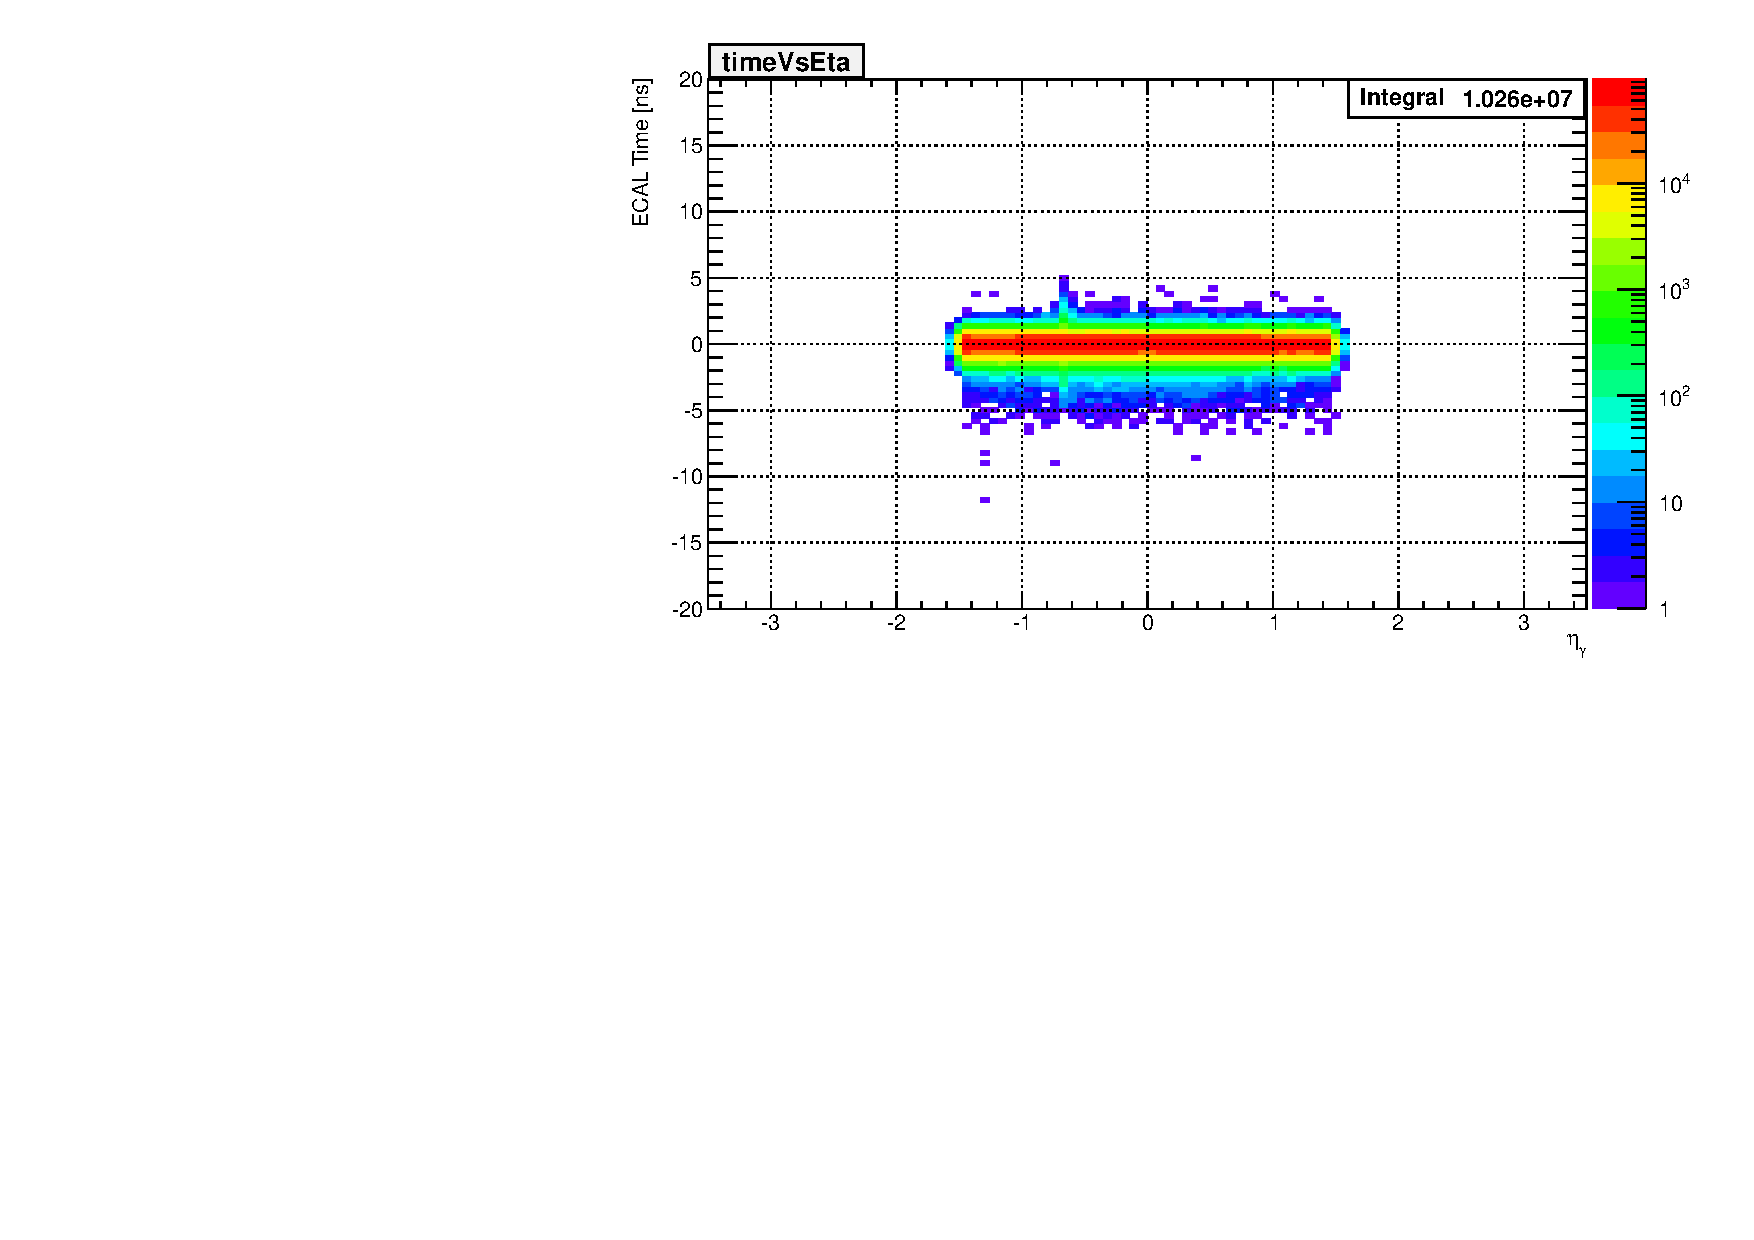
\includegraphics[height=0.340\textwidth, width=0.5\textwidth]
{THESISPLOTS/ZCandidates_TimeVsEta.pdf}}
\mbox{
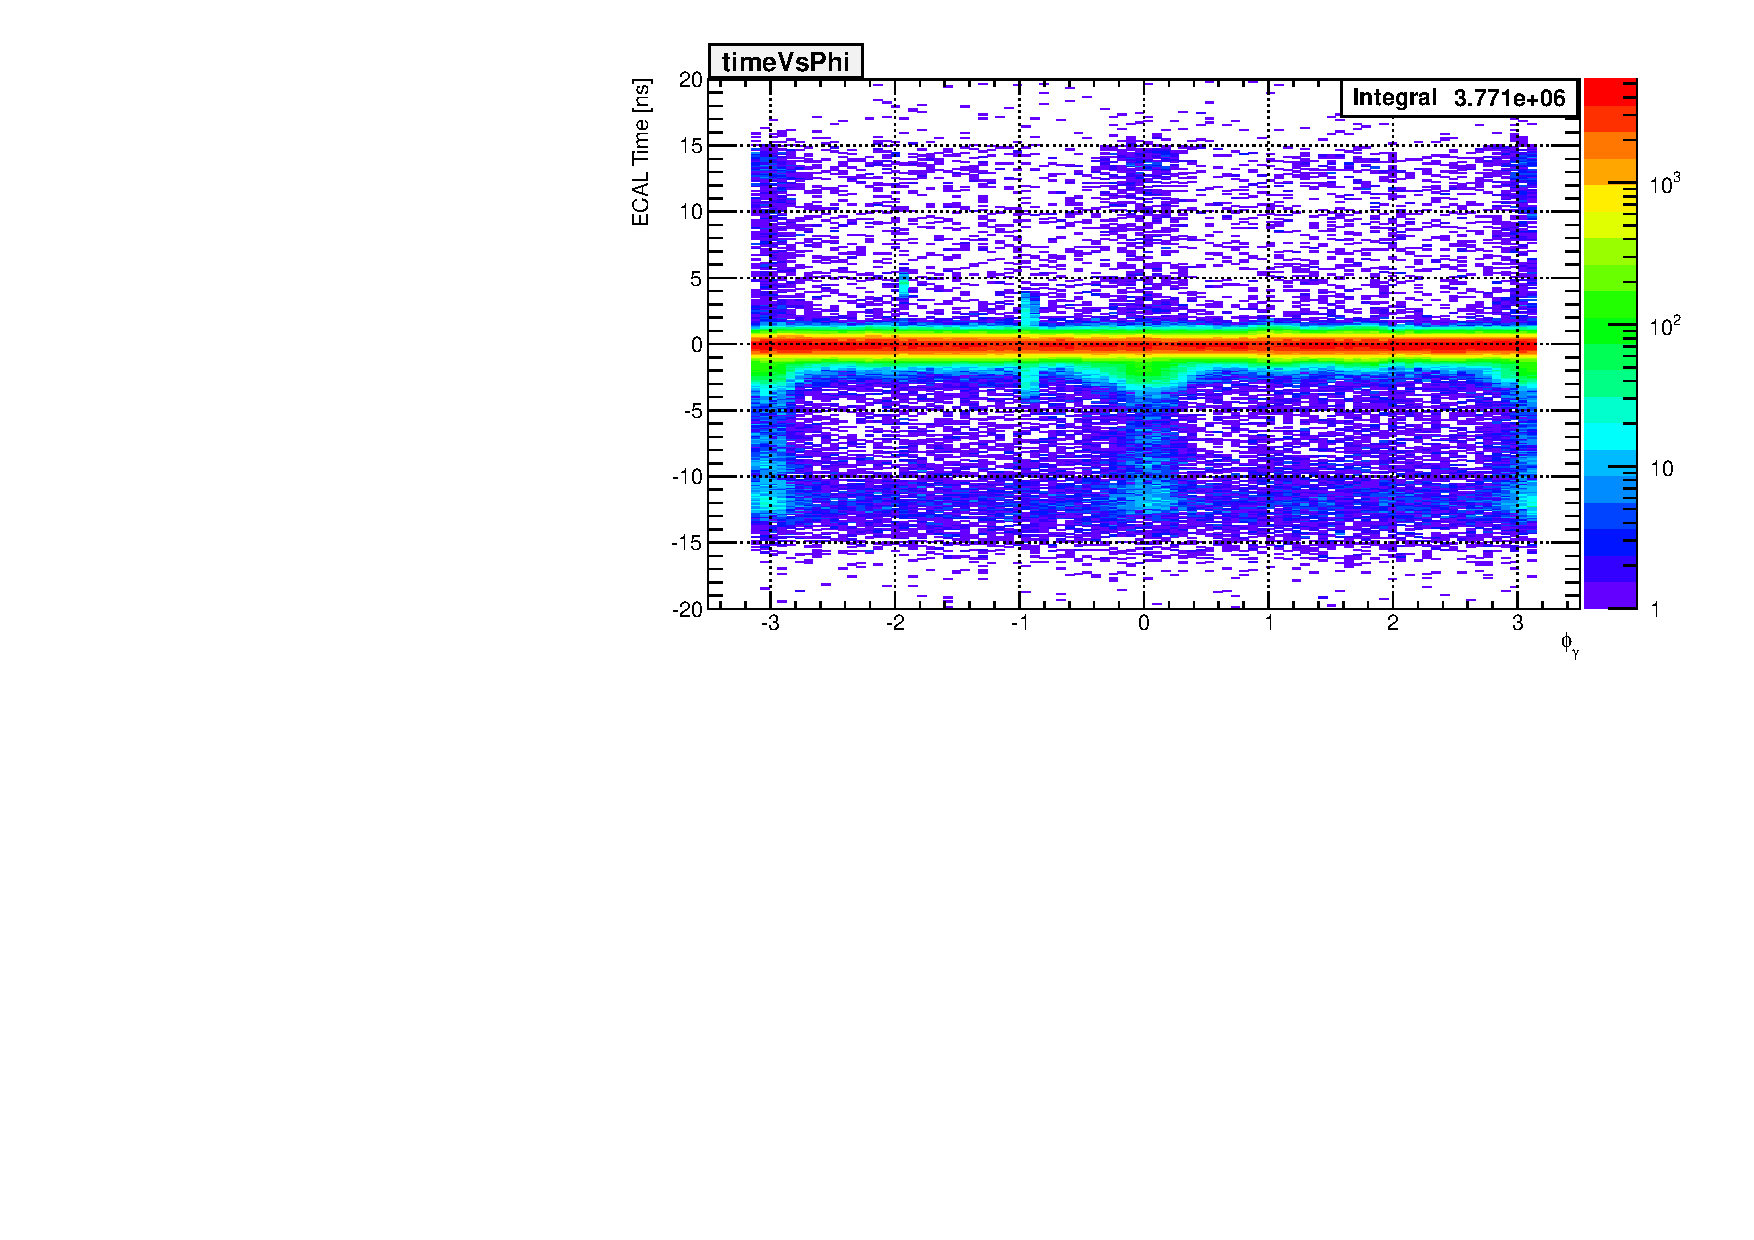
\includegraphics[height=0.340\textwidth, width=0.5\textwidth]{THESISPLOTS/SinglePhotonDataSet-TimeVsPhiEB.pdf}
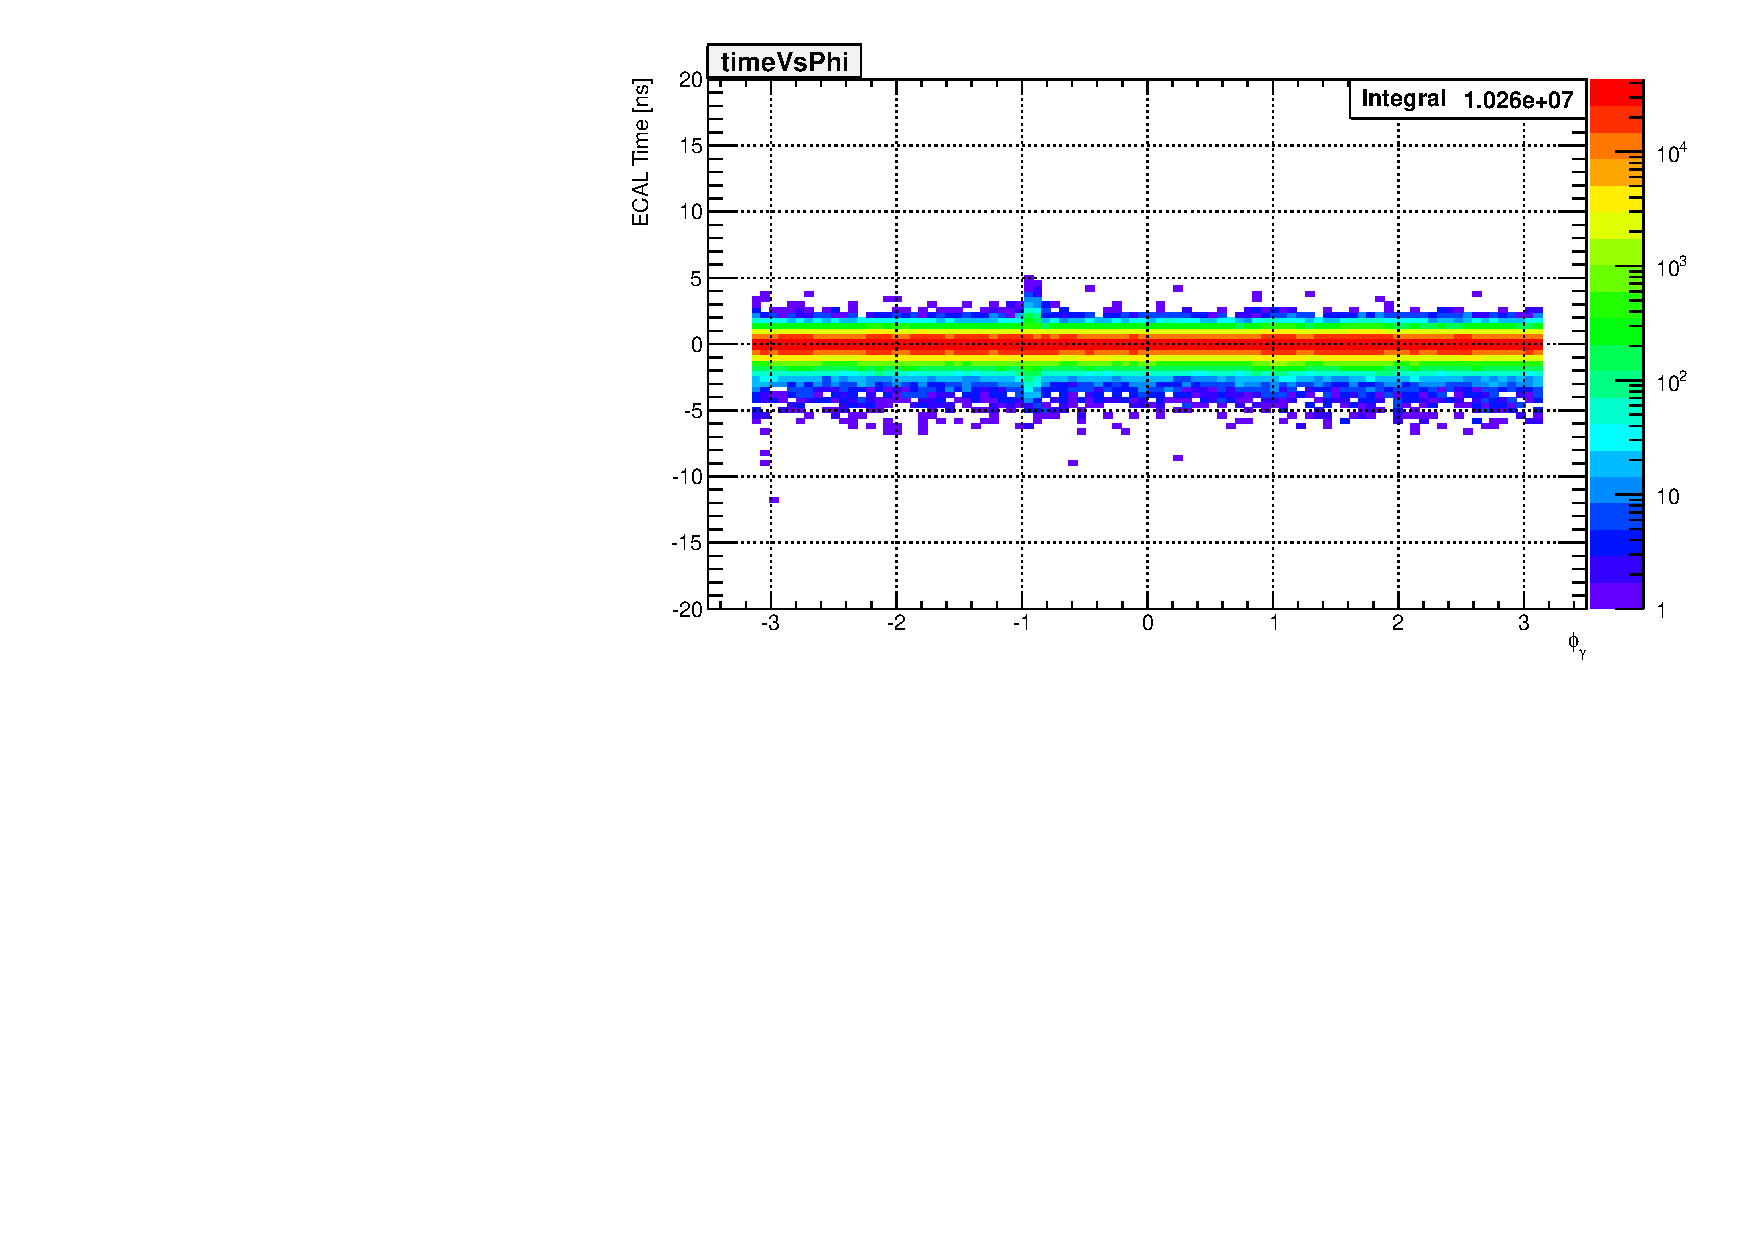
\includegraphics[height=0.340\textwidth, width=0.5\textwidth]{THESISPLOTS/ZCandidates_TimeVsPhi.pdf}}
\captionof{figure}{ECAL time $Vs$ $\eta$~(top plots) and $Vs$ $\phi$~(bottom plots) for photon candidates from \texttt{SinglePhoton} dataset~(left) compared to electron candidates from the \texttt{DoubleElectron} dataset~(right). All photons or electron candidates are in barrel subdetector. Most of the photons with $\phi = 0, \pm \pi$ are halo photons which are not observed in the $\PZ$ boson candidate sample.}
\label{fig:Elec}
\end{center}
\end{minipage}

\vspace{5mm}
The di-electron mass~(left plots) and electron arrival time~(right plots) of both electron candidates of the \PZ boson for signal~(blue) and sideband~(red) events is shown in Figure \ref{fig:Zmass}. The out-of-time background contribution to the true \PZ events sample is estimated using a \textit{sideband subtraction method} described as follows:
\begin{itemize}
\item We fit the di-electron candidate mass distribution of the sideband control sample with a polynomial function(see top plots of Figure  \ref{fig:collZ}) to extract the background template.
\item Using the background template, we obtain a scale factor as 
\begin{equation}
\mbox{Scale Factor} = \frac{N}{M_{1} + M_{2}},
\end{equation}
shown in the bottom plot of Figure \ref{fig:collZ}, which we used to determine the correct contribution of the background events to the signal event sample.
\item After scaling the electrons arrival ECAL time distribution~(red distribution on the bottom right plot in Figure \ref{fig:Zmass}) of the sideband control sample using the extracted scale factor, we subtract the scaled time distribution from the time distribution~(blue distribution of right plot in Figure \ref{fig:Zmass}) of \PZ electron candidates from the signal sample. The resulting ECAL time distribution, shown in Figure \ref{fig:Ztime} is the time distribution from true \PZ events. This ECAL time distribution is used to estimate the number of events with out-of-time electromagnetic particles from collision.
\item The ratio of the total number of events with the electron ECAL time, $t > 3$~ns, to those with electron ECAL time, $|t| < 2$~ns, \ie $ N_{t > 3~ns}/ N_{|t| < 2.0~ns}$, gives an estimate of the fraction of out-of-time background events from collision. 
\end{itemize}  

\vspace{5mm}
\begin{minipage}{0.90\linewidth} 
\begin{center}
\mbox{
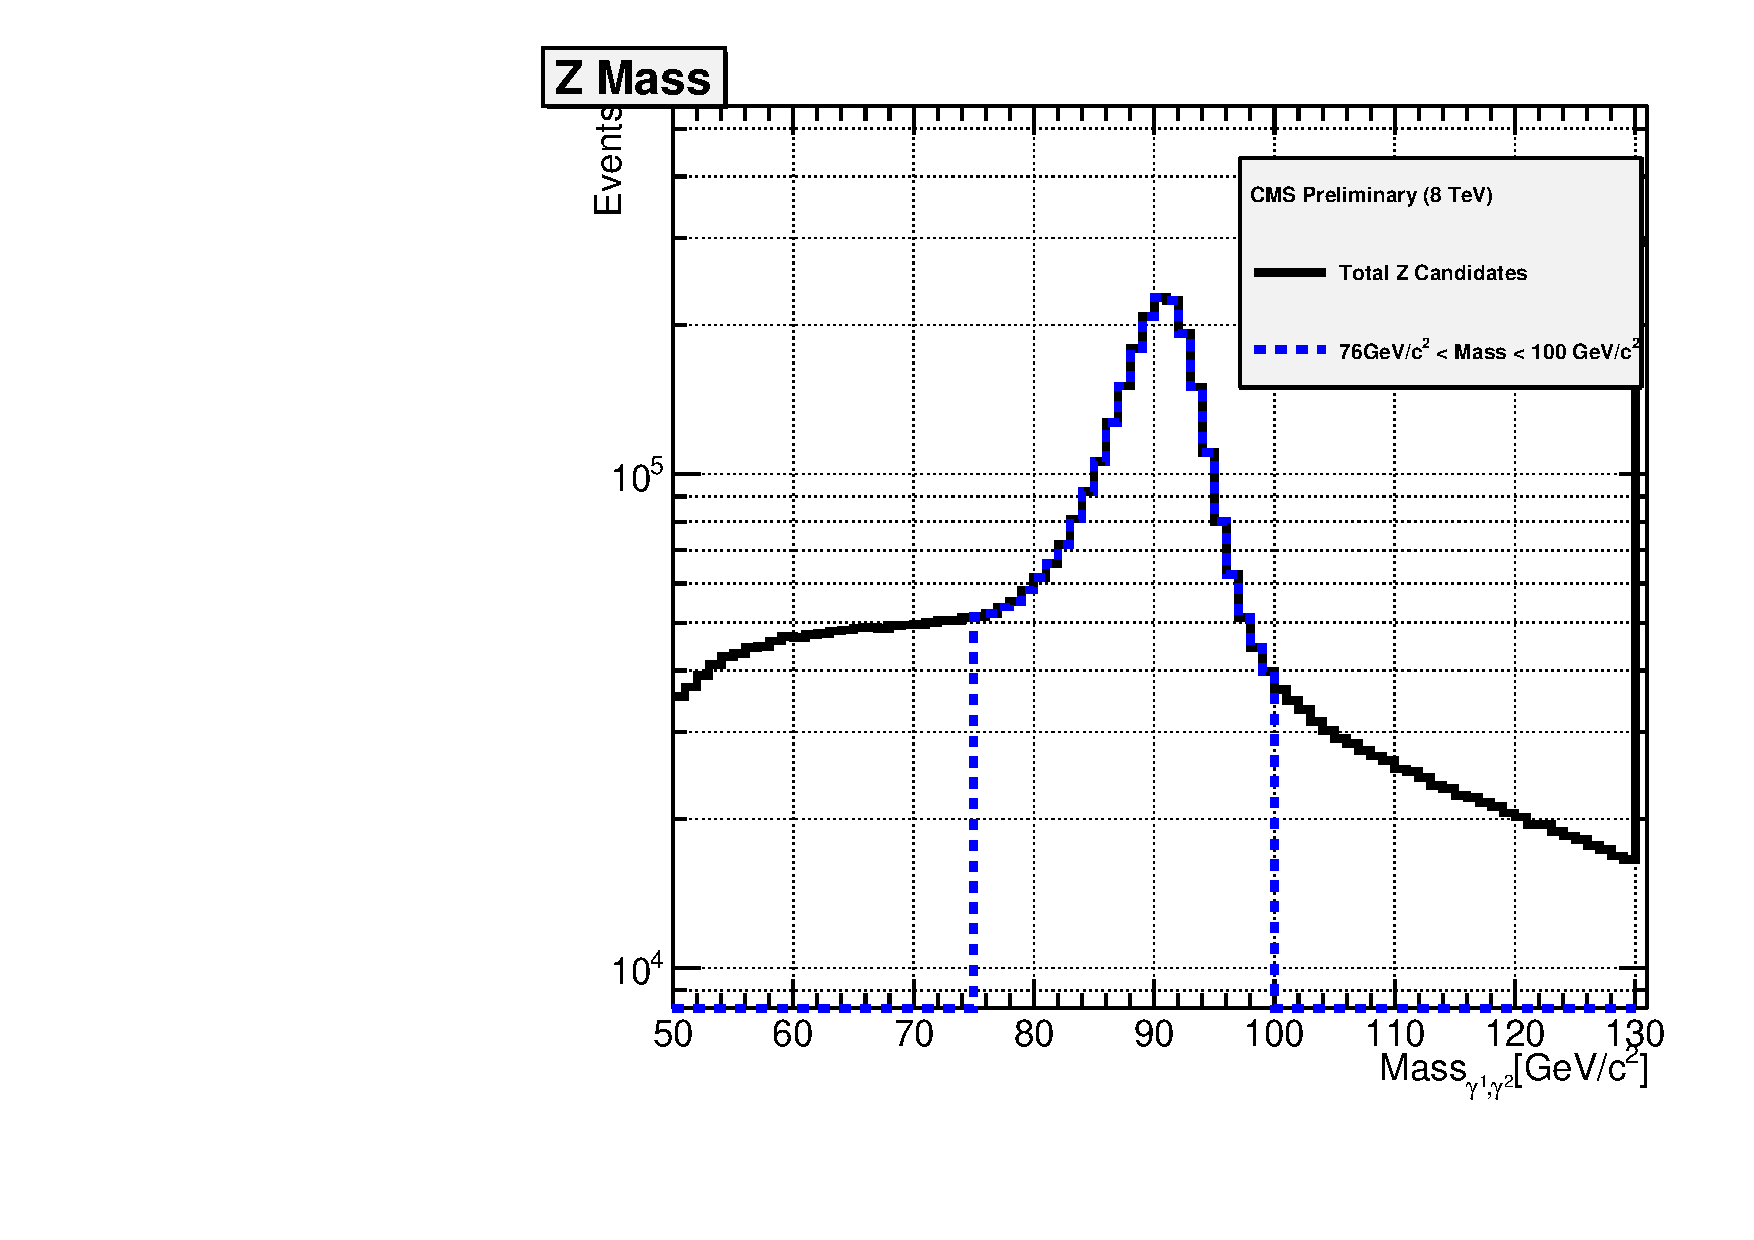
\includegraphics[height=0.55\textwidth, width=0.5\textwidth]{THESISPLOTS/Z-CandidateOverLay-SignalMass.pdf}
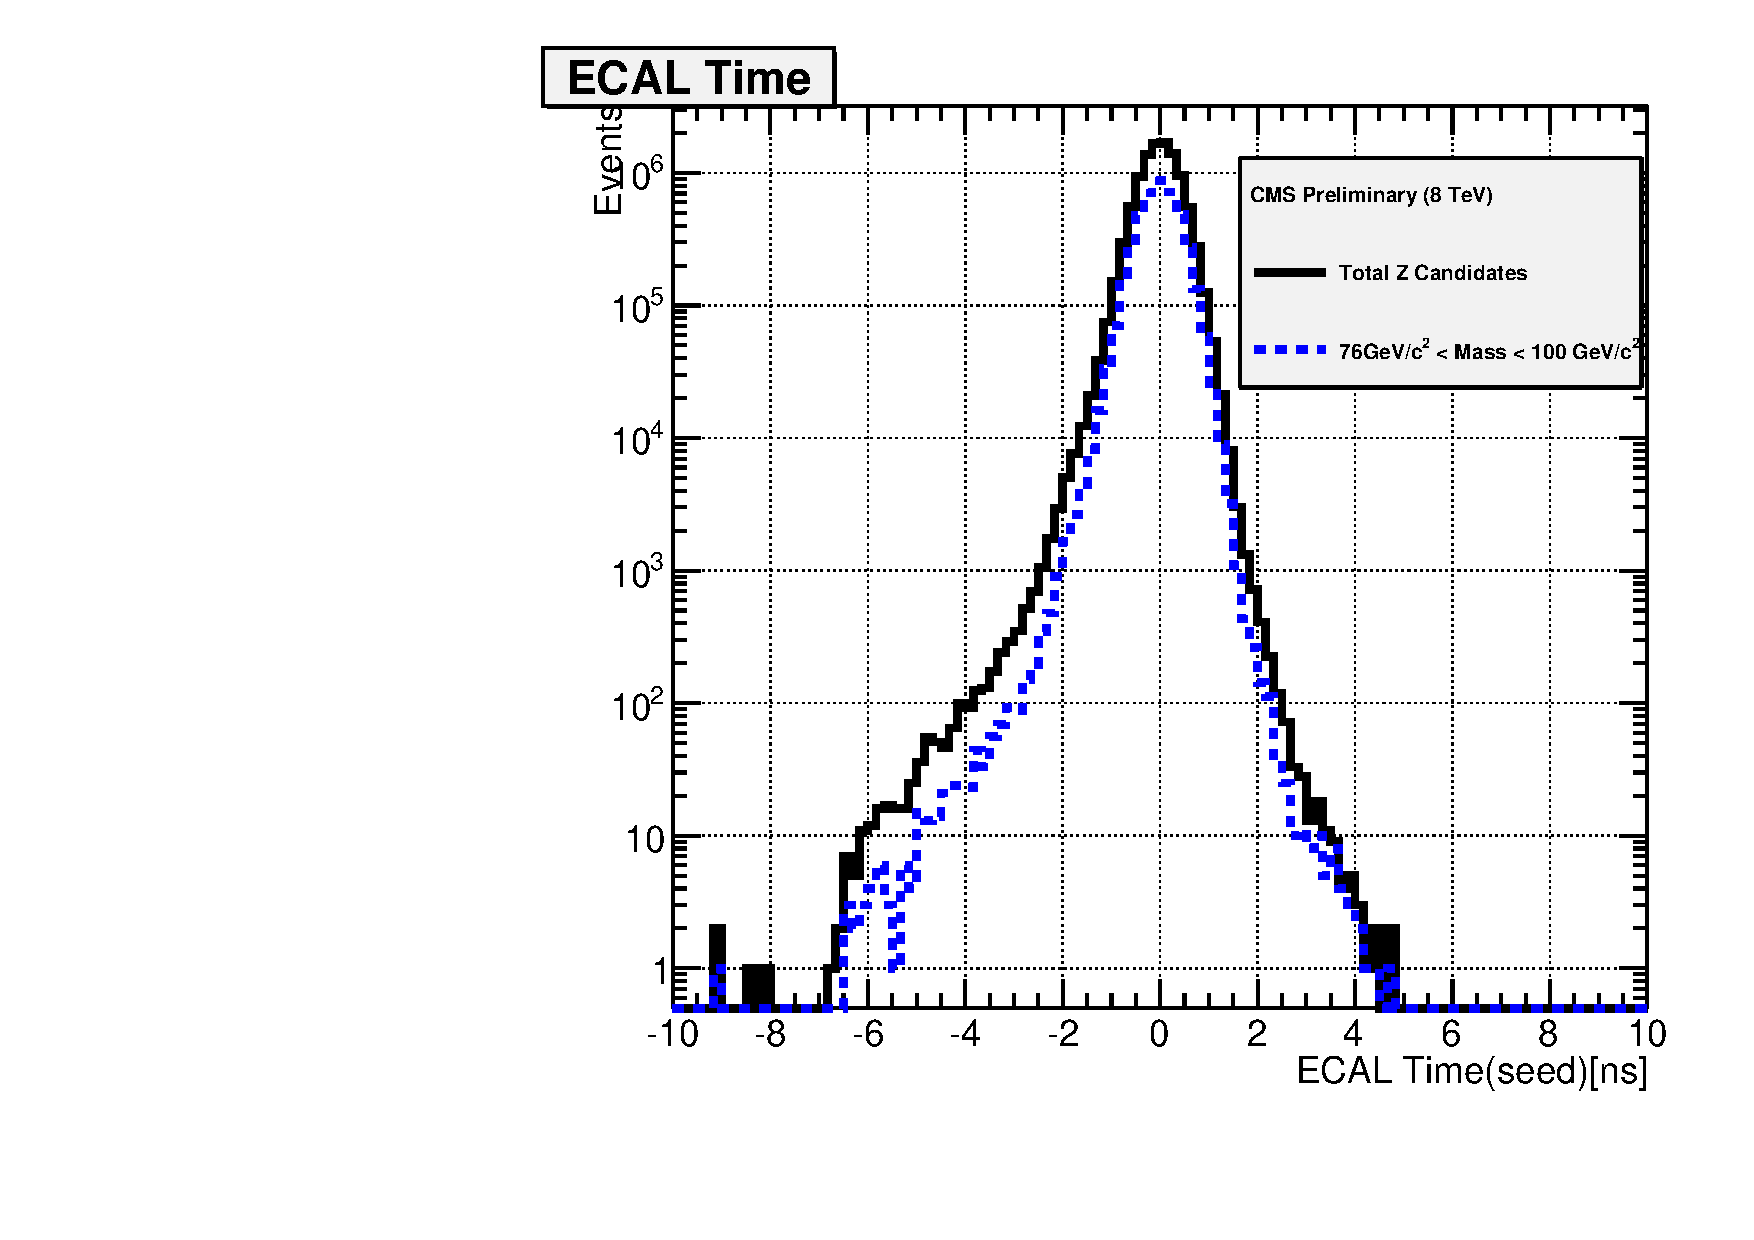
\includegraphics[height=0.55\textwidth, width=0.5\textwidth]{THESISPLOTS/Z-CandidateOverLay-SignalTime.pdf}}
\mbox{
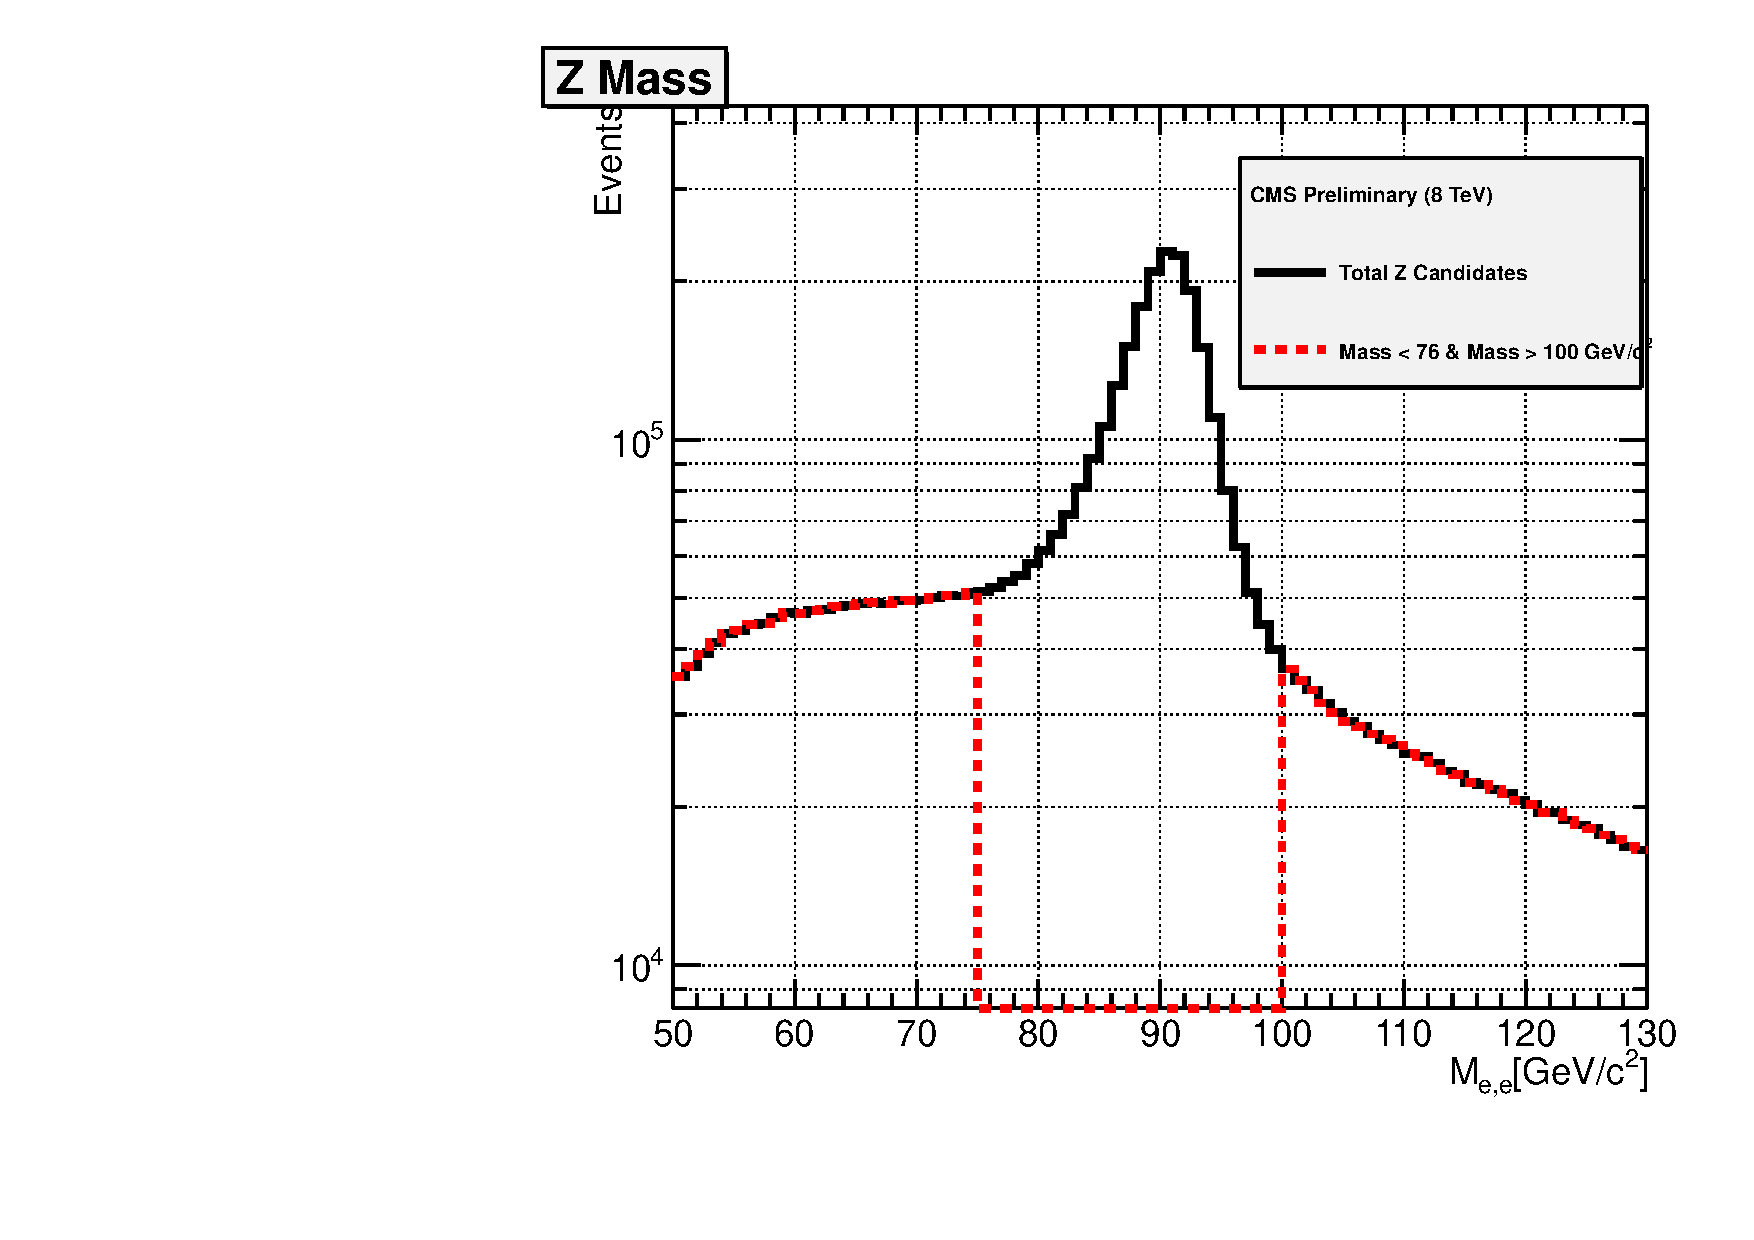
\includegraphics[height=0.55\textwidth, width=0.5\textwidth]{THESISPLOTS/Z-CandidateOverLay-BackgroundMass.pdf}
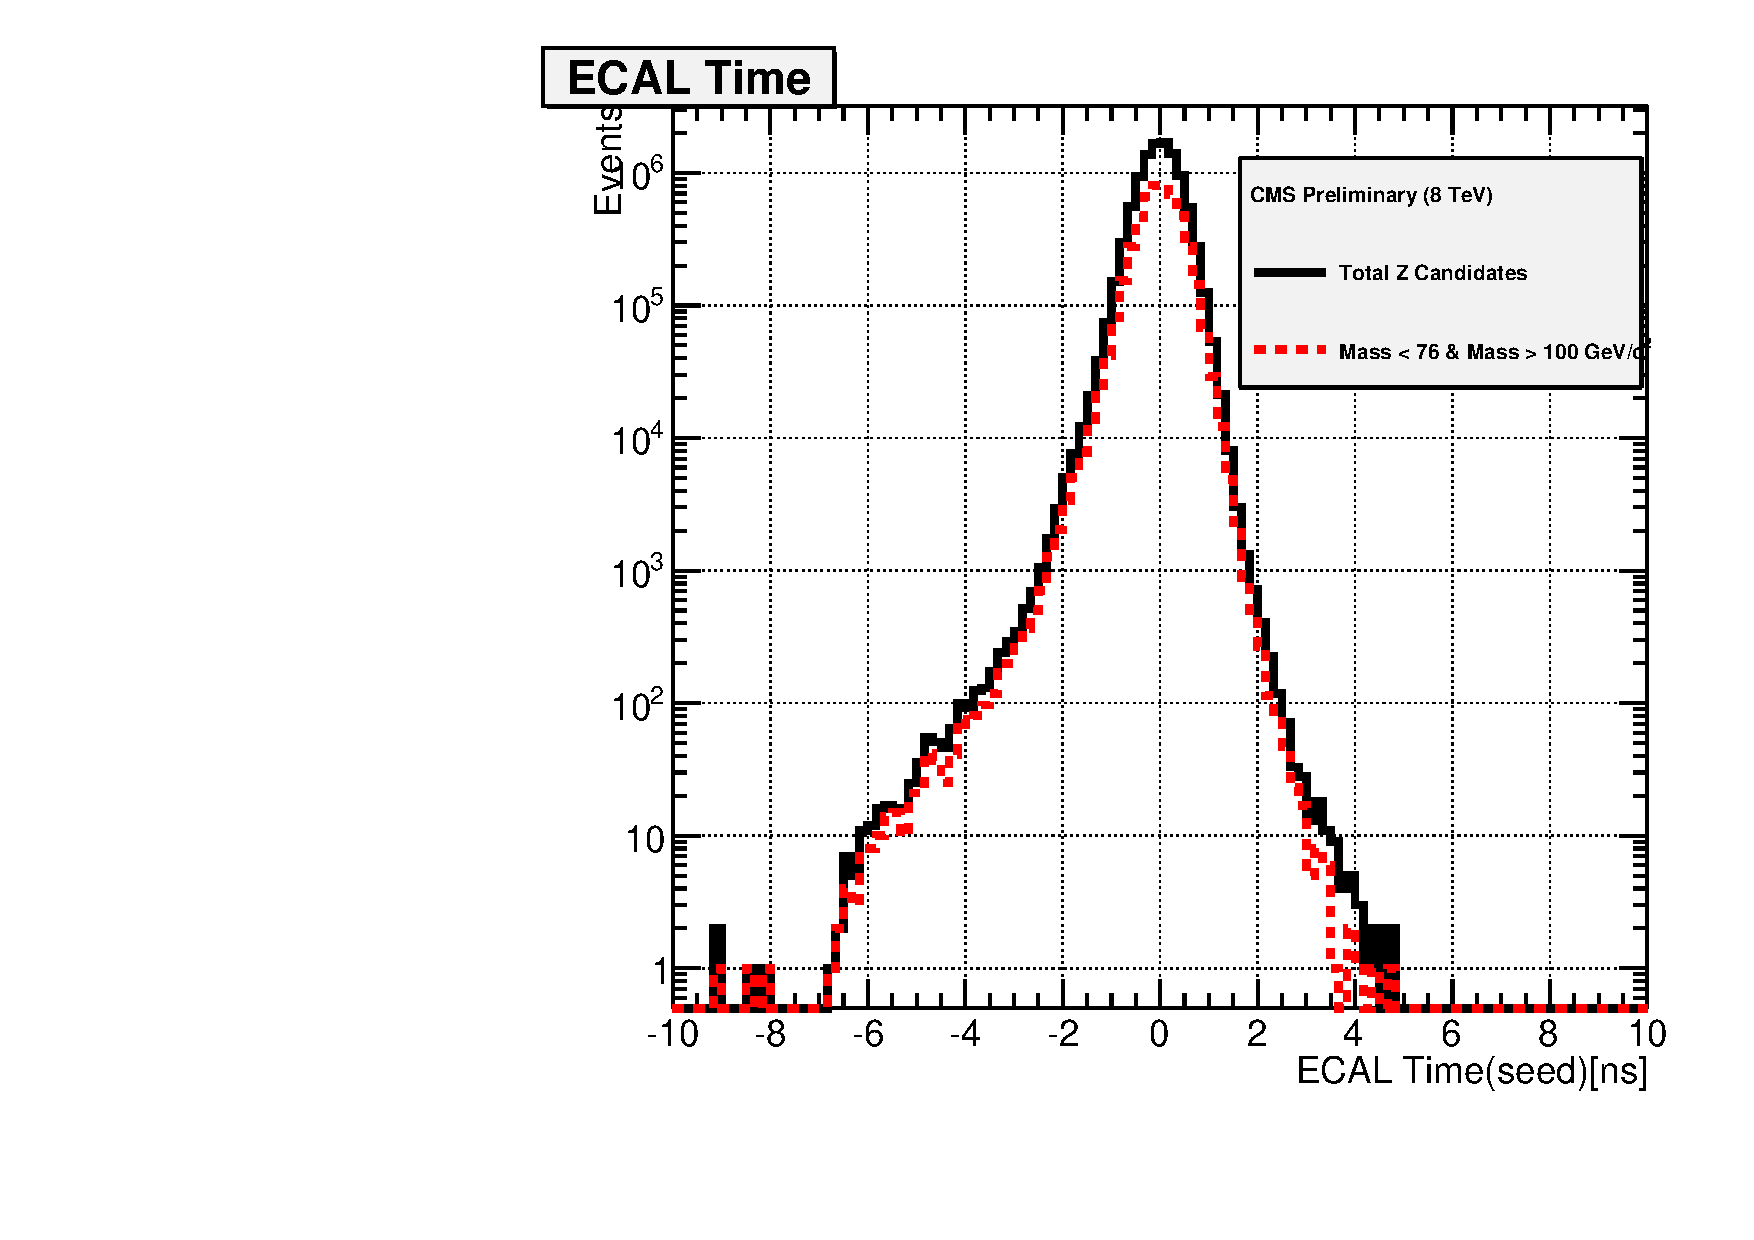
\includegraphics[height=0.55\textwidth, width=0.5\textwidth]{/home/tensr/Documents/TEN-HEP-PHD-THESIS/PHD_THESIS/PHD/THESISPLOTS/Z-CandidateOverLay-BackgroundTime.pdf}}
\captionof{figure}{Di-electron mass distribution~(left) and the time~(right) of the two electron candidates for the signal \textcolor{blue}{$76 < m_{\EE} < 100$}\GeVcc $\PZ$ boson sample and for sideband sample~(\textcolor{red}{$50 < m_{\EE} < 76$}\GeVcc and \textcolor{red}{$ 100 < m_{\EE} < 130$}\GeVcc). Events are from the \texttt{Single/DoubleElectron} data sample.}
\label{fig:Zmass}
\end{center}
\end{minipage}

\vspace{5mm}
\begin{minipage}{0.90\linewidth} 
\begin{center}
\mbox{
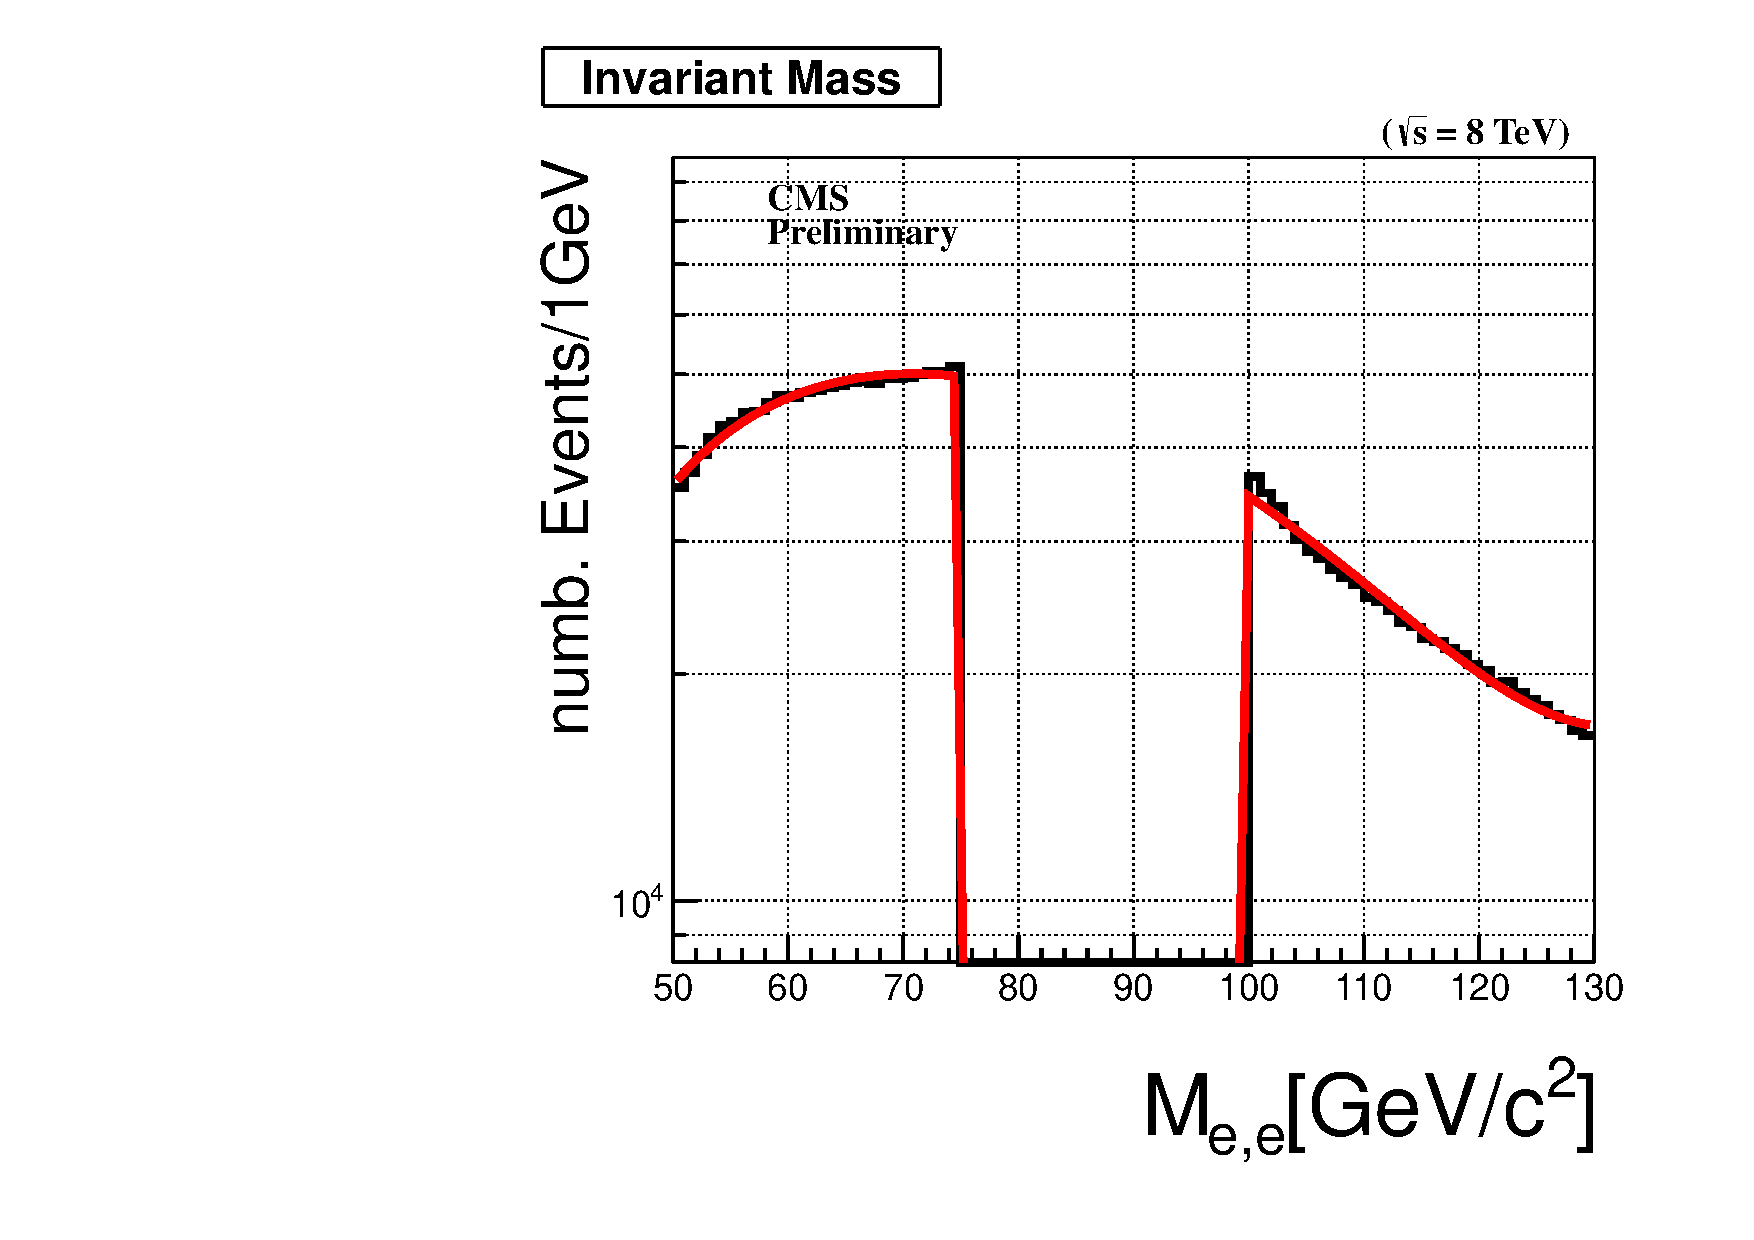
\includegraphics[height=0.50\textwidth, width=0.5\textwidth]{THESISPLOTS/Uncleaned-di-Photon-ZMass-Fit-DoubleElectron-Run2012A.pdf}
\includegraphics[height=0.50\textwidth, width=0.5\textwidth]{THESISPLOTS/Background_In_ZMass-From-Di-Photon.pdf}}
\mbox{
\includegraphics[height=0.55\textwidth, width=0.8\textwidth]{THESISPLOTS/ZBackground_SF.png}
%\includegraphics[height=6cm, width=0.5\textwidth]{THESISPLOTS/CMS_Slice.png}
}
\captionof{figure}{\textit{Top}: Polynomial fit~(red \& blue lines) of the di-electron invariant mass of candidate \PZ events for the sideband control sample~(left) only and all \PZ events~(right). \textit{Bottom:} Fitting the total \PZ event sample with template extracted from fitting the sideband CS to extract the scale factor use for estimating the background event contribution in true \PZ signal events sample.}
\label{fig:collZ}
\end{center}
\end{minipage}

\vspace{5mm}
  The estimated ratio for out-of-time events to in-time collision events for the final time distribution of signal electron candidates after the normalized sideband subtraction, shown in Figure \ref{fig:Ztime} is about, $N_{t > 3~ns}/ N_{|t| < 2.0~ns} = 1.29 ^{+0.374}_{-0.325} \times 10^{-5}$.
\par
To obtain an estimate of the number of background events from collisions in the signal control sample \textsf{D}, $N^{col}_{D}$, of the \PSneutralinoOne decay, we multiply this estimated ratio to the total number of in-time events~(CS \textsf{$I$}), shown in Table \ref{tab:RESULT}, passing our final signal event selections requirements, which is $28282$. This gives $N^{col}_{D} = 0.366^{+0.106}_{-0.092}$ events. Comparing this to the value obtained with the \textsf{ABCD} method, which is $\frac{28283}{1446522} = 0.0391^{+0.039}_{-0.047}$ events, we find that the two methods of estimating the number of background events from collision are not exactly equal. 
\par
We cannot interpret this inequality  as a disagreement between both methods for estimating the number of background events from collision. On the contrary, this non-agreement can be explained. We have not applied any \MET selection requirements for the \PZ candidate events selection. A simple cut in missing transverse energy, $\MET > 60$\GeV, could further reduce the estimated ratio, $N_{t > 3~ns}/ N_{|t| < 2.0~ns}$, to a very smaller number than what we got. In fact, the smallness of this ratio confirms our speculation that indeed the contribution from collision events with out-of-time electromagnetic particles to our background events is almost negligible~(less than a single event) such that the uncertainties on the ratio of out-of-time to in-time events used in our \textsf{ABCD} collision background estimation is irrelevant. This means, the number $N^{col}_{D} = 0.366^{+0.106}_{-0.092}$, can be used for our estimated number of background events from collision and our final results will not change by a lot.
  
\vspace{5mm}
\begin{minipage}{0.90\linewidth} 
\begin{center}
%\mbox{
\includegraphics[height=0.55\textwidth, width=0.7\textwidth]{THESISPLOTS/Seed-Time-From-Uncleaned-di-photon-Mass-Fit-DoubleElectron-Run2012A.pdf}
%\includegraphics[scale=0.2]{THESISPLOTS/CMS_Slice.png}
\captionof{figure}{ECAL time distribution of genuine $\PZ$ bosons after background contribution is subtracted.}
\label{fig:Ztime}
\end{center}
\end{minipage}


\section{Systematic Studies}
Our event selection comprise of the following selection cuts: photon \pt greater than 80\GeVc, jet \pt greater than 35\GeVc and missing energy greater than 60\GeV. The same selection requirements applied to our MC signal event sample should guarantee a good event selection efficiency. Any difference in the photon \pt, jet \pt and missing transverse energy between MC and data, will be a source of systematic uncertainties on the efficiency of selecting signal events. These uncertainties can come from quantities like jet energy scale~(JES), jet energy resolution~(JER), electron-photon energy scale, instrumentation related and missed or energy deposits not clustered during missing transverse energy reconstruction, photon ECAL arrival time bias and ECAL time resolution. The different sources of uncertainties considered in this analysis is presented in Table \ref{tab:SYST}. We obtain these uncertainties by varying the nominal values of each quantity, while keeping the others fixed, by $1\sigma$ deviation and counting the number of events passing our event selection requirements. Our largest uncertainty is from ECAL timing bias on the absolute reference time~(zero ns) of the ECAL timing used for measuring the photon arrival time. This has the largest impact on our analysis since our analysis is based on counting the number of events with photon ECAL time above $3$~ns. The next largest uncertainties are from energy deposits not clustered. This affects the photon energy scale, missing energy scale,  jet energy scale and resolution.
\newline
The uncertainty on the photon energy scale in the barrel was estimated to be 4.0\%  based on measuring the photon energy of events with $Z\rightarrow \mu\mu\gamma$ decay, where the muon radiates a photon in a process known as the final-state radiation~(FSR)\cite{PES}.  
\newline
The uncertainty on the \MET resolution uses a conservative estimate from \MET measurements in QCD events \cite{METRES}. 
\newline
The uncertainty on the ECAL time resolution was obtained by comparing the mean time of photons of events from $\gamma +$ jet MC sample to events from data with photon ECAL time, $|t_{\gamma}| < 2$~ns. The difference is found to be of the order of 200~ps per event. 
\newline
The systematic uncertainty on luminosity measurement has the recommended value of $2.2$\% provided by CMS and LHC luminosity measurements while the uncertainty from pardon density functions~(PDF) is evaluated using the re-weighting technique which uses the Master Equation of CTEQ65 model set described in \cite{PDF}.
\par
Another important source of systematic is in the selection of the background control samples and our background estimation and individual systematic in the tagging and mistagging of non-collision background and estimating background contributions from collisions. We combined these separate uncertainty contributions into a single background estimation uncertainty referred here as our background estimation uncertain. 
However, since our background estimation is data-driven, most of the uncertainties arising due to systematic can be neglected~(less than 1\% impact) as the cancel out.
This is our largest source of uncertainty in our analysis which we estimate to vary it upward by 223\% and downward by 51\% as a statistical uncertainty in the \textsf{ABCD} background estimation method. The large background statistical uncertainty is due to very low event statistics. However, despite the large background estimation uncertainty, the signal selection uncertainties are the most significant uncertainties which impact our final results. These uncertainties are used as nuissance parameters in the calculation of the upper limit on observed signal cross-section~($\sigma_{UL}$).

\vspace{5mm}
\begin{minipage}{0.90\linewidth} 
\begin{center}
%\begin{table}[ht]
%\renewcommand\arraystretch{1.2}
\begin{tabular}{c c}
\toprule
\hline
\bfseries{Source} & \bfseries {Uncertainty(\%)}\\
\hline
\toprule
\texttt{ECAL absolute time }~(0.0~ns) & $<10.0$\% \\
\texttt{ECAL time resolution}~(0.5~ns) & $<5.0$\% \\
\texttt{Unclustered energy deposits} & $<9.0$\% \\
\texttt{Photon energy scale}  & $< 4.0$\% \\
\texttt{Jet energy scale}~(JES)  & $< 9.0$\% \\
\texttt{Jet energy resolution}~(JER) &$ <9.0$\% \\
\texttt{\MET resolution} & $ <2.8$\%  \\
\texttt{PDF uncertainty} & $< 1.70$\% \\
\hline
\toprule
\texttt{Background estimation uncertainty} &$51.0$\% to 223\% \\
\hline 
\texttt{Luminosity}~(4.5\%) & $< 2.2$\% \\
\hline
\bottomrule
\end{tabular}
\captionof{table}{Summary of systematic uncertainties for signal efficiency and background estimation in this analysis and applied to our final results.}
\label{tab:SYST}
%\end{table}
\end{center}
\end{minipage}


\section{Results}
After running our analysis on the SinglePhoton data samples requiring events with at least 2 jets, at least one photon with ECAL time  $ 3.0 < t_{\gamma} < 13.0$~ns, ${\ETslash}^{\gamma}\hspace{0.15cm} > 60$\GeV, and $\ETslash\hspace{0.15cm} > 60$\GeV, we observed a single event passing all our event selection requirements as a signal event. This event has one photon and two jets. The photon has a transverse momentum  of 224\GeVc and an ECAL time of 12.17~ns.
\newline
Our final expected number of background events estimated is $0.093^{+0.301}_{-0.047}$. This number was computed as
\begin{align*} 
 N_{B}^{col} &= \frac{28283}{605496} \times 3 = 0.140^{+0.108}_{-0.061} \\
 N_{D}^{col} &= \frac{28283}{605496} \times 2 = 0.093^{+0.093}_{-0.047} \\
 N_{D}^{Total} &= \left( \frac{1 - 0.14}{3}\times 0\right) +  0.093 = 0.093^{+0.301}_{-0.047}.
\end{align*}
using the event yields and background events vetoed presented in Table \ref{tab:RESULT}. 

\vspace{5mm}
\begin{minipage}{0.90\linewidth} 
\begin{center}
\begin{tabular}{c| c| c| c| c }
\toprule
 \hline
\bfseries{Control Sample} & Yield & Beam Halo & Cosmic & Spike \\
\hline
\toprule
\textsf{D} & 1 & 0 & 0 & 0 \\
\textsc{C} & 0 & 2 & 1& 0  \\
\textsf{B} & 1 & 1&  1 &  1\\
\textsf{A} & 3 & 6 & 0 & 0\\
\hline\hline
\textsf{$A^{\prime}$}& 2 & 0 & 0 & 0\\ 
\textsf{$C^{\prime}$}& 4 & 0 & 0 & 0\\  
\textsf{$I$} & 28283 & -& - & -\\    
\textsf{$I^{\prime}$}&  669013 & - & - & \\       
\hline
\bottomrule
\end{tabular}
\captionof{table}{Event yields used in our final background estimation for signal candidate events with at least a single photon and at least 2 jets, ${\ETslash}^{\gamma}\hspace{0.15cm} > 60$\GeV, and $\ETslash\hspace{0.15cm} > 60$\GeV. }
\label{tab:RESULT} 
\end{center}
\end{minipage}

\vspace{5mm} 
With no significant excess over expected number of background events, we find upper limits on the number of event counts at 95\% confidence limit using the statistical CLs limit finding method.
%\paragraph*{}\mbox{}\\
%\begin{minipage}{\linewidth} 
%\begin{center}
%\centering
%%\begin{tabular}{|c| c| c|}
%%%\mbox{Fake Rate }
%%\toprule
%%\hline
%%\bfseries{Non-Collision} & $\mathbf{{\ETslash}^{\gamma}\hspace{0.15cm}} < 60$\GeV & $\mathbf{{\ETslash}^{\gamma}\hspace{0.15cm}} > 60$\GeV \\
%%\hline
%% $3.0 < t_{\gamma} < 13.0$~ns & \textsf{$C$}($0$) & ~\textsf{$D$}(\textcolor{blue}{$1$}) \\
%% $-10.0 < t_{\gamma} < -3.0$~ns & \textsf{$A$}($5$) & ~\textsf{$B$}($1$) \\
%%\hline \hline
%%\bfseries{Collision} & $\mathbf{\ETslash\hspace{0.15cm}} < 60$\GeV & $\mathbf{\ETslash\hspace{0.15cm}} > 60$\GeV \\
%%\hline 
%% $3.0 < t_{\gamma} < 13.0$~ns & \textsf{$D^{\prime}$}($5$) & ~\textsf{D} \textcolor{red}{$0.0888 ^{+0.1869}_{-0.0444}$} \\
%% $-2.0 < t_{\gamma} < 2.0$~ns & \textsf{$F^{\prime}$}($657663$) & ~\textsf{$F$}($30242$) \\
%% $-10.0 < t_{\gamma} < -3.0$~ns & \textsf{$B^{\prime}$}($1$) & ~\textsf{$B$} $0.23 ^{+0.092}_{-0.118}$) \\
%%\hline
%%\bottomrule
%%\end{tabular}
%%\captionof{table}{Result of observed events and estimated background from signal sample, events with at least $2$-jets. Numbers in bracket represent our observed number of events while numbers not is bracket are our expected number of background events estimated using \textsf{ABCD} method.}
%%\label{tab:RF} 
%%\end{center}
%%\end{minipage}
%%\paragraph*{}\mbox{}\\
\label{Search_Analysis_chapter}